% Drones que buscan personas, para principiantes: la simulación del Tarot 650
% que busca personas en el bosque. Compila con pdfLaTeX (por omisión en Overleaf), XeLaTeX o LuaLaTeX.
\documentclass[11pt,letterpaper,oneside,openany]{book}

\usepackage{iftex}
\ifPDFTeX
  \usepackage[utf8]{inputenc}
  \usepackage[T1]{fontenc}
  \usepackage{lmodern}
\else
  \usepackage{fontspec}
\fi
\usepackage[spanish,es-noshorthands,es-tabla]{babel}
\usepackage[margin=2.4cm]{geometry}
\usepackage{amsmath,amssymb}
\usepackage{graphicx}
\usepackage{booktabs,tabularx,array,longtable}
\usepackage{enumitem}
\usepackage[dvipsnames]{xcolor}
\usepackage[most]{tcolorbox}
\usepackage{listings}
\usepackage{tikz}
\usetikzlibrary{arrows.meta,positioning,shapes.geometric,shapes.misc,fit,calc,decorations.pathmorphing}
\usepackage{caption}
\usepackage{float}
\usepackage{xurl}
\usepackage[colorlinks=true,linkcolor=NavyBlue,urlcolor=NavyBlue,citecolor=NavyBlue]{hyperref}

\graphicspath{{figuras/}}
\setlist{itemsep=2pt,topsep=4pt}
\setlength{\parindent}{0pt}
\setlength{\parskip}{6pt}
\setlength{\emergencystretch}{3em}
\captionsetup{font=small,labelfont=bf}
\urlstyle{tt}

% Rutas, archivos, nodos y tópicos en monoespaciado (con _ y / sin escapar).
\newcommand{\cod}[1]{\expandafter\nolinkurl\expandafter{\detokenize{#1}}}
\newcommand{\sgn}{\operatorname{sgn}}
\newcommand{\Sgn}{\operatorname{Sgn}}

\lstset{basicstyle=\ttfamily\footnotesize,columns=fullflexible,keepspaces=true,breaklines=true,
        frame=single,rulecolor=\color{black!25},backgroundcolor=\color{black!3},
        xleftmargin=4pt,xrightmargin=4pt,aboveskip=6pt,belowskip=6pt,
        showstringspaces=false,upquote=true,
        literate={á}{{\'a}}1 {é}{{\'e}}1 {í}{{\'i}}1 {ó}{{\'o}}1 {ú}{{\'u}}1
                 {Á}{{\'A}}1 {É}{{\'E}}1 {Í}{{\'I}}1 {Ó}{{\'O}}1 {Ú}{{\'U}}1
                 {ñ}{{\~n}}1 {Ñ}{{\~N}}1 {ü}{{\"u}}1 {¿}{{?`}}1 {¡}{{!`}}1
                 {°}{{$^\circ$}}1 {²}{{$^2$}}1 {·}{{$\cdot$}}1 {→}{{$\rightarrow$}}1
                 {×}{{$\times$}}1 {±}{{$\pm$}}1 {—}{{---}}1 {–}{{--}}1}
\lstdefinestyle{bash}{language=bash,morekeywords={ros2,colcon,source,sudo,git,gz,python3}}
\lstdefinestyle{py}{language=Python,keywordstyle=\color{NavyBlue}\bfseries,commentstyle=\color{black!55}\itshape,
                    stringstyle=\color{BrickRed}}
\lstdefinestyle{xml}{language=XML,keywordstyle=\color{NavyBlue},stringstyle=\color{BrickRed}}

% Recuadros del libro.
\tcbset{enhanced,breakable,boxrule=0.6pt,arc=2pt,left=6pt,right=6pt,top=4pt,bottom=4pt,fonttitle=\bfseries}
\newtcolorbox{nota}{colback=NavyBlue!4,colframe=NavyBlue!70!black,title=Nota}
\newtcolorbox{aviso}{colback=BrickRed!5,colframe=BrickRed!70!black,title=Cuidado}
\newtcolorbox{leccion}{colback=ForestGreen!5,colframe=ForestGreen!70!black,title=Problema encontrado y cómo se resolvió}
\newtcolorbox{recuerda}{colback=Goldenrod!10,colframe=Goldenrod!80!black,title=Recuerda}
\newtcolorbox{consejo}{colback=Cyan!5,colframe=Cyan!60!black,title=Consejo}
\newtcolorbox{tecnico}{colback=black!3,colframe=black!45,title=Para curiosos (te lo puedes saltar)}
\newtcolorbox{ejemplo}[1][]{colback=Orchid!5,colframe=Orchid!70!black,title=Ejemplo de la vida diaria#1}
\newtcolorbox{ejercicio}{colback=Peach!8,colframe=Peach!80!black,title=Pruébalo tú}
\newtcolorbox{enpocas}{colback=ForestGreen!4,colframe=ForestGreen!50!black,title=En este capítulo}

\title{\textbf{Drones que buscan personas}\\[4pt]
\textbf{para principiantes}\\[10pt]
\Large Percepción, estimación y control de un Tarot 650 que busca\\ personas perdidas en el bosque por sí solo\\[8pt]
\large ROS 2 Jazzy · Gazebo Harmonic · PX4 · ArduPilot · YOLO26}
\author{Dr.\ Jairo Olguín Roque\\
FES Acatlán, UNAM}
\date{Octubre de 2026}

\begin{document}
\frontmatter
\maketitle
\tableofcontents
\chapter{Cómo usar este libro}

\section*{¿Para quién es?}

Para cualquier persona que quiera entender, desde cero, cómo funciona un dron que busca personas por
sí solo: estudiantes, ingenieros de otras áreas o curiosos. No necesitas saber de drones, de visión
computacional ni de redes neuronales. Ayuda saber usar una computadora con Linux y recordar algo de
física y matemáticas de bachillerato; cuando haga falta algo más, se explica en el momento.

El libro cuenta una historia concreta: una simulación en la que un dron Tarot 650 despega, recorre en
franjas un bosque de $120\times120$ metros, mira hacia abajo con su cámara, reconoce a las personas
con una red neuronal (YOLO), calcula en qué punto del suelo está cada una, avisa sus coordenadas GPS y
aterriza. El vuelo lo controla un piloto automático real (PX4 o ArduPilot) o una red neuronal
entrenada para imitarlo. Cada pieza de esa historia es una excusa para explicar un concepto.

\section*{Cómo está organizado}

\begin{description}
  \item[Parte I. Lo básico.] Qué es un dron y cómo vuela, la física mínima, qué es una simulación,
        y ROS~2 y PX4, que conectan todas las piezas.
  \item[Parte II. Ver y ubicar.] Qué es una imagen, cómo aprende una red neuronal a reconocer
        personas y cómo se pasa de un recuadro en la imagen a un punto en el mapa, con su incertidumbre.
  \item[Parte III. El control.] Cómo se mantiene el dron en su ruta: control en cascada y una red
        neuronal que aprende a volar imitando al piloto automático.
  \item[Parte IV. Construir la simulación.] La instalación y cómo se metieron en Gazebo el Tarot 650, su
        cámara, el bosque y las personas.
  \item[Parte V. La misión.] Cómo el dron decide qué hacer: el barrido, la re-observación de casos
        dudosos, los avisos GPS y la evasión de obstáculos, con PX4 o con ArduPilot.
  \item[Parte VI. Experimentos y manos a la obra.] Cómo se diseña y analiza una campaña de cientos de
        vuelos, un tutorial para tu primer vuelo y la referencia de órdenes.
\end{description}

Al final hay un \textbf{glosario}. Si solo quieres usar la simulación, ve directo al
capítulo~\ref{cap:primer-vuelo}.

\section*{Los recuadros}

\begin{recuerda}
Lo más importante del tema, en pocas palabras.
\end{recuerda}
\begin{consejo}
Trucos prácticos que ahorran tiempo o problemas.
\end{consejo}
\begin{ejemplo}
Una comparación con algo cotidiano.
\end{ejemplo}
\begin{tecnico}
Detalles matemáticos o de programación que puedes saltarte la primera vez.
\end{tecnico}
\begin{aviso}
Errores fáciles de cometer.
\end{aviso}
\begin{leccion}
Problemas reales que aparecieron durante el desarrollo y cómo se resolvieron.
\end{leccion}
\begin{ejercicio}
Algo que puedes hacer en la simulación para comprobar lo que acabas de leer.
\end{ejercicio}

\section*{Convenciones}

\begin{itemize}
  \item Las órdenes de terminal van en recuadros grises:
\begin{lstlisting}[style=bash]
ros2 launch mision simulacion.launch.py
\end{lstlisting}
  \item Nombres de archivos, programas y tópicos en letra de máquina: \cod{localizador_node}.
  \item \cod{~} es tu carpeta personal. El paquete principal está en \cod{~/ros2_ws/src/mision}.
  \item Distancias en metros, tiempos en segundos, ángulos en radianes o grados (se indica).
\end{itemize}


\mainmatter
\part{Antes de despegar: lo básico}
\chapter{El proyecto de un vistazo}

\section{El problema}

Cuando una persona se pierde en un bosque, encontrarla pronto puede salvarle la vida. Un dron con
cámara recorre en minutos lo que a una brigada a pie le tomaría horas, y lo hace sin arriesgar a
nadie. Pero desde el aire una persona ocupa unos pocos píxeles, las copas de los árboles la tapan, la
luz cambia y el viento mueve al dron. Para que el dron sirva hay que resolver tres preguntas:
\begin{enumerate}
  \item \textbf{¿Hay alguien en la imagen?} (percepción: detector de personas);
  \item \textbf{¿Dónde está en el mapa, y qué tan seguro estoy?} (estimación: localización en el
        terreno y fusión de observaciones);
  \item \textbf{¿Cómo recorro el bosque sin perder a nadie?} (control y misión).
\end{enumerate}

\section{Qué hace la simulación}

\begin{itemize}
  \item \textbf{Bosque por factores:} se genera un bosque con tres niveles de cobertura de copas (15,
        45 y 75~\%), dos condiciones de luz (sol alto o sombras largas), con o sin viento, y de una a
        tres personas de pie, sentadas o acostadas en lugares al azar.
  \item \textbf{Dron:} un x500 de PX4 de 2.114~kg con una cámara de $1280\times960$ que mira hacia
        abajo, una IMU, GPS y un LiDAR.
  \item \textbf{Piloto:} PX4~1.17 o ArduCopter~4.7, en SITL (el mismo programa que volaría en el dron
        real).
  \item \textbf{Controlador:} la cascada del piloto automático o una red neuronal 15-64-32-4 que
        imita a la cascada y corre dentro de PX4 (módulo \emph{Neural Control}).
  \item \textbf{Detector:} YOLO26s ajustado con 3000 imágenes del simulador (AP50 = 0.954).
  \item \textbf{Localizador:} corta el rayo de cada detección con el suelo, calcula su elipse de error
        y fusiona las detecciones de una misma persona.
  \item \textbf{Misión:} barrido en franjas a 30~m, re-observación de candidatas dudosas, avisos GPS,
        aterrizaje y métricas (personas localizadas, falsas alarmas, error).
\end{itemize}

\section{Arquitectura}

\begin{figure}[H]
\centering
\begin{tikzpicture}[
  nodo/.style={draw,rounded corners,fill=#1,minimum width=3.1cm,minimum height=1cm,align=center,font=\small},
  nodo/.default=white,
  flecha/.style={-{Stealth[length=2.5mm]},thick},
  et/.style={font=\scriptsize\ttfamily,fill=white,inner sep=1pt}]
  \node[nodo=orange!15,minimum width=4.2cm,minimum height=2cm] (gz) at (0,0) {\textbf{Gazebo Harmonic}\\ bosque, x500, cámara,\\ LiDAR, viento};
  \node[nodo=red!10] (px4) at (6,0) {\textbf{PX4 SITL}\\ (o ArduCopter)\\ cascada o red neuronal};
  \node[nodo=black!5] (dds) at (6,-2.6) {agente\\ uXRCE-DDS};
  \node[nodo=black!5] (puente) at (0,-2.6) {\cod{ros_gz_bridge}};
  \node[nodo=blue!10] (det) at (-3.4,-5) {\cod{detector_node}\\ YOLO26s (GPU)};
  \node[nodo=green!12] (loc) at (1,-5) {\cod{localizador_node}\\ rayo--terreno y fusión};
  \node[nodo=green!12] (mis) at (6,-5) {\cod{mision_node}\\ barrido, avisos};
  \node[nodo=yellow!15] (gps) at (6,-7.3) {aviso GPS\\ \cod{/personas/*}};
  \node[nodo=black!5] (gcs) at (10.2,-2.6) {MAVProxy\\ consola y mapa};
  \draw[flecha] (gz) -- node[et,above]{motores, sensores} (px4);
  \draw[flecha] (px4) -- node[et,right]{odometría} (dds);
  \draw[flecha] (gz) -- (puente);
  \draw[flecha] (puente) -| node[et,pos=0.7]{/camera} (det);
  \draw[flecha] (det) -- node[et,above]{/detecciones} (loc);
  \draw[flecha] (dds) -| node[et,pos=0.75,left]{odometría} (loc);
  \draw[flecha] (loc) -- node[et,above]{/personas/candidatas} (mis);
  \draw[flecha] (mis) -- node[et,right]{consignas} (dds);
  \draw[flecha] (mis) -- (gps);
  \draw[flecha] (px4.east) -| node[et,pos=0.3,above]{MAVLink} (gcs);
\end{tikzpicture}
\caption{Programas y tópicos principales. La cadena es \emph{imagen $\rightarrow$ detección
$\rightarrow$ localización $\rightarrow$ fusión $\rightarrow$ decisión $\rightarrow$ consigna
$\rightarrow$ control}.}
\label{fig:arquitectura}
\end{figure}

\begin{figure}[H]
\centering
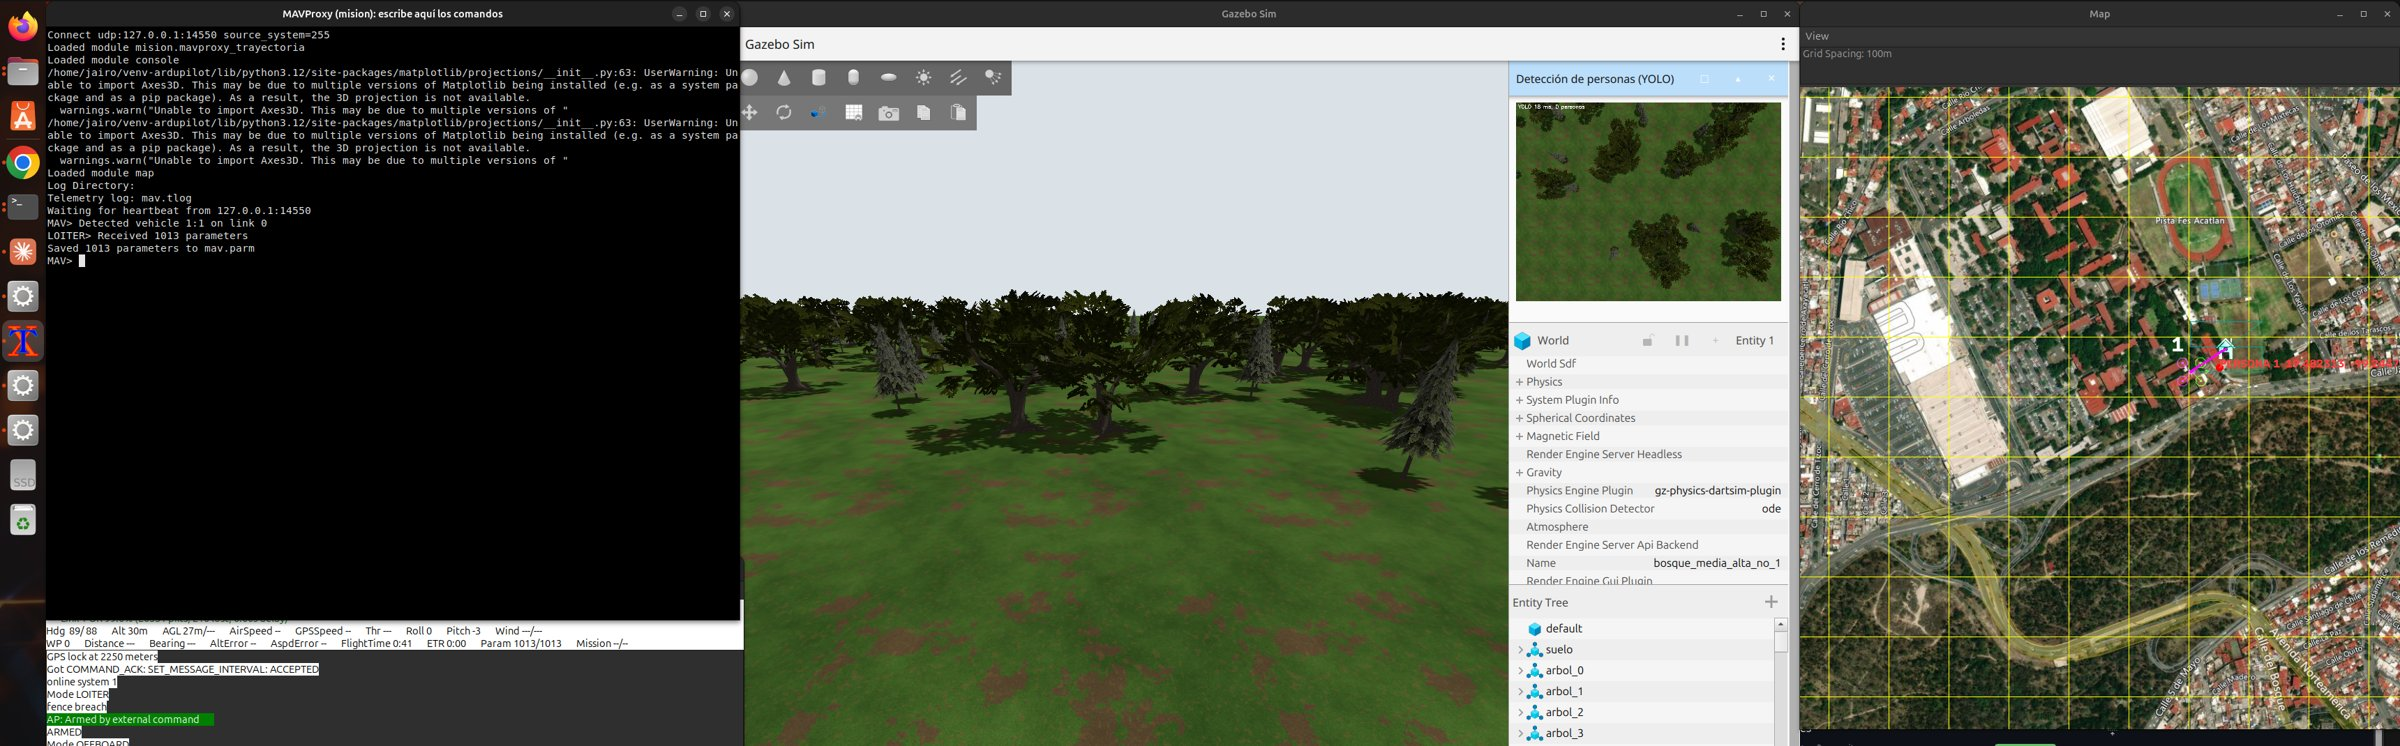
\includegraphics[width=\textwidth]{pantalla_mavproxy.jpg}
\caption{La simulación en marcha: a la izquierda la terminal y la consola de MAVProxy (la estación de
tierra), al centro Gazebo con el panel de detección, a la derecha el mapa con la persona 1 ya
localizada.}
\end{figure}

\section{Un vuelo completo}

\begin{figure}[H]
\centering
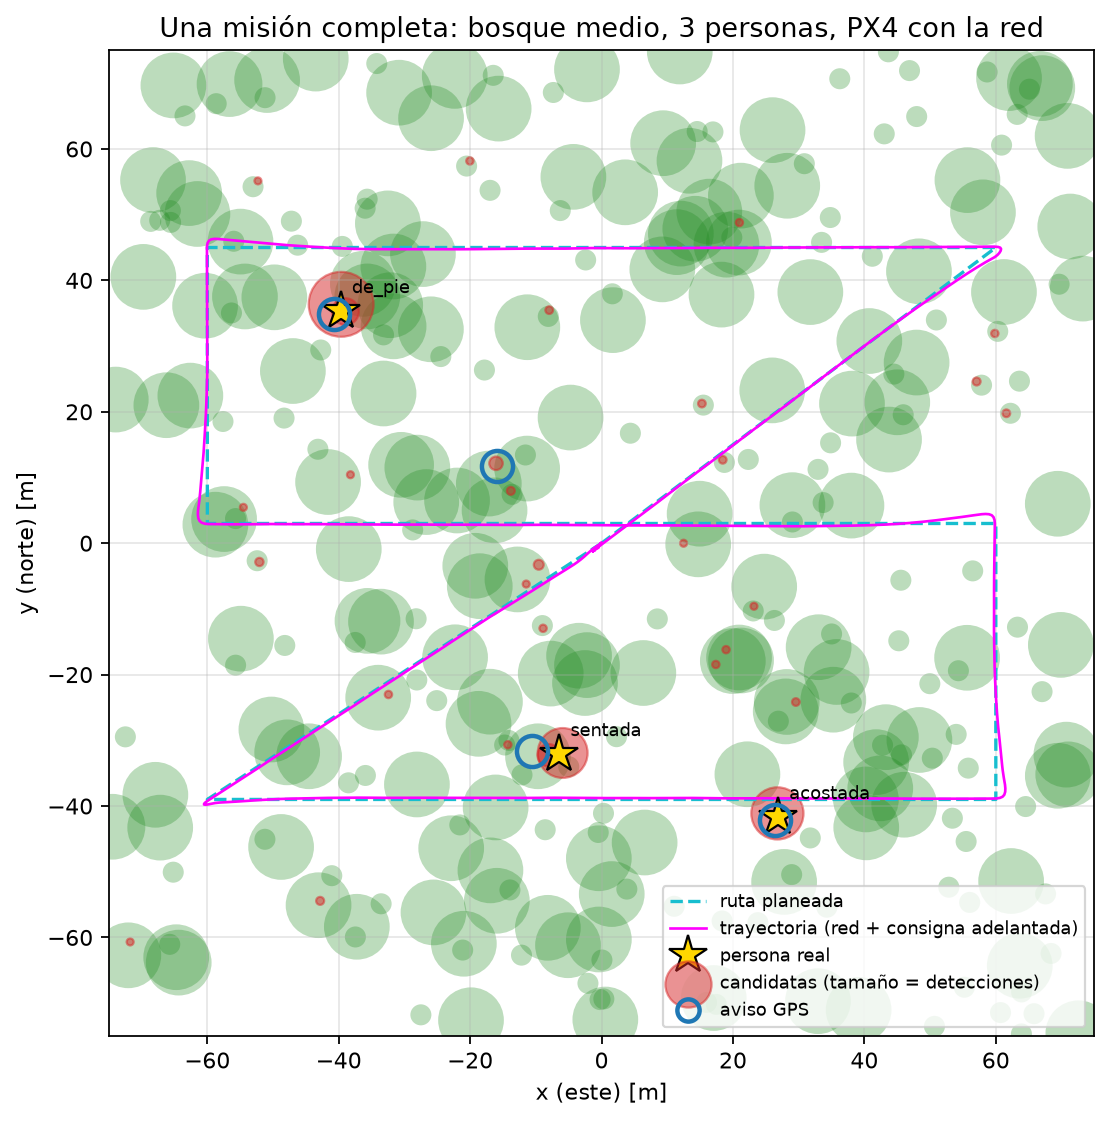
\includegraphics[width=0.85\textwidth]{mision_mapa.png}
\caption{Una misión real de la simulación, vista desde arriba: el bosque (círculos verdes), la ruta
planeada, lo que voló el dron, las candidatas que fue juntando el localizador, las tres personas
reales y los avisos GPS.}
\label{fig:mision-mapa}
\end{figure}

La figura~\ref{fig:mision-mapa} resume todo el libro: el dron sigue franjas paralelas, el detector ve
personas y también cosas que no lo son (puntos rojos), el localizador junta las detecciones de cada
lugar, y la misión avisa cuando una candidata ya está confirmada. Las tres personas se encontraron con
menos de 1~m de error; también hubo un aviso falso entre unos robles. Entender por qué pasa cada cosa
es el objetivo de las páginas que siguen.

\section{Convenciones de marcos}

\begin{itemize}
  \item \textbf{Mundo:} ENU (\emph{x} este, \emph{y} norte, \emph{z} arriba), en metros, con origen en
        el centro del bosque. PX4 y ArduPilot usan NED: $N=y$, $E=x$, $D=-z$.
  \item \textbf{Cuerpo:} en ROS FLU (\emph{x} al frente, \emph{y} a la izquierda, \emph{z} arriba); en
        PX4 FRD (\emph{y} a la derecha, \emph{z} abajo).
  \item El mundo está georreferenciado en 19.4826° N, 99.2447° O, 2250~m, así que el GPS del dron y
        los avisos dan coordenadas reales.
\end{itemize}

\chapter{¿Qué es un dron y cómo vuela?}

\begin{enpocas}
Las partes de un cuadrirrotor, por qué vuela, cómo sube, avanza y gira con solo cambiar la velocidad
de sus cuatro motores, y cómo es el x500 que usamos.
\end{enpocas}

\section{Drones, multirrotores y cuadrirrotores}

``Dron'' es el nombre popular de un \textbf{vehículo aéreo no tripulado} (UAV, por sus siglas en
inglés): una aeronave sin piloto a bordo. Puede ser un avión de ala fija, un helicóptero o, el caso
más común, un \textbf{multirrotor}: una aeronave con varias hélices horizontales. El de cuatro
hélices se llama \textbf{cuadrirrotor} o \textbf{cuadricóptero}.

¿Por qué cuatro? Porque es el número mínimo con el que se puede controlar todo el movimiento sin
piezas móviles más que los propios motores: no hay alerones, timones ni ``plato cíclico'' como en
un helicóptero. Eso los hace baratos, robustos y fáciles de reparar; a cambio, son inestables por
naturaleza: sin una computadora que corrija cientos de veces por segundo, se voltean.

\begin{recuerda}
Un cuadrirrotor no tiene superficies de control. Todo lo que hace (subir, inclinarse, girar) lo
consigue cambiando la velocidad de sus cuatro motores. Por eso el \emph{control} es el corazón del
dron.
\end{recuerda}

\section{Las partes}

\begin{figure}[H]
\centering
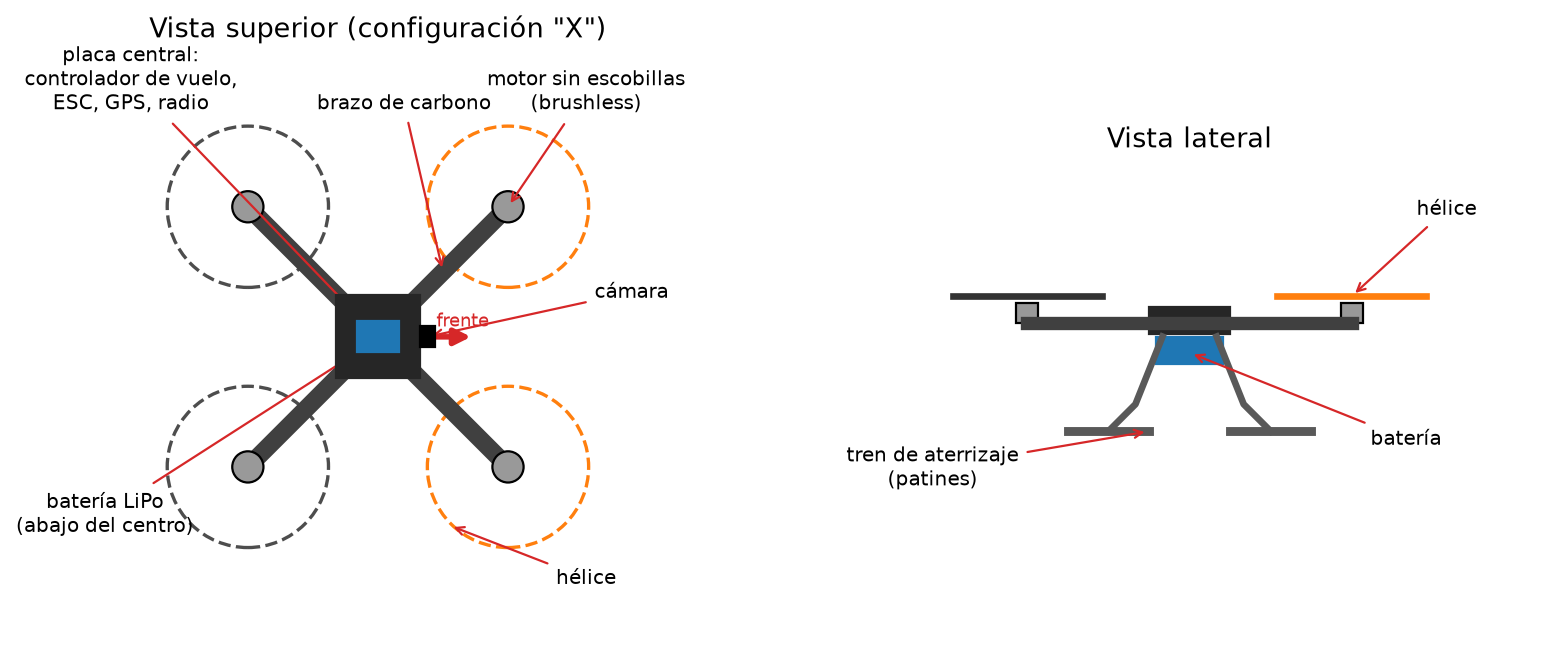
\includegraphics[width=\textwidth]{c_partes.png}
\caption{Partes de un cuadrirrotor como el x500.}
\label{fig:partes}
\end{figure}

\begin{description}
  \item[Marco (frame).] La estructura: una placa central y cuatro brazos. En el x500 son de fibra de
        carbono, ligera y rígida; mide 500~mm entre motores opuestos.
  \item[Motores sin escobillas (brushless).] Motores eléctricos trifásicos muy eficientes. Su constante
        KV dice cuántas revoluciones por minuto da por cada volt.
  \item[ESC (controlador electrónico de velocidad).] Uno por motor. Recibe una orden (``gira a tanto'')
        y genera las corrientes trifásicas para lograrlo.
  \item[Hélices.] Convierten el giro en empuje. Se describen con dos números: diámetro y paso, en
        pulgadas. Las del x500 son de $13\times4.5$: 13'' de diámetro (33~cm) y 4.5'' de paso (lo que
        avanzarían en una vuelta si se ``atornillaran'' en el aire).
  \item[Batería LiPo.] Polímero de litio: mucha energía para su peso. Se describen por el número de
        celdas en serie (4S, 6S: 3.7~V cada una) y su capacidad en mAh.
  \item[Controlador de vuelo.] La computadora a bordo: lee los sensores y decide la velocidad de cada
        motor cientos de veces por segundo. Puede llevar ArduPilot o PX4. En nuestra simulación ese
        papel lo hacen PX4 o ArduPilot en SITL (y, en el modo neuronal, una red dentro de PX4).
  \item[Sensores.] IMU (acelerómetros y giroscopios: cómo se mueve y gira), barómetro (altura),
        magnetómetro (brújula), GPS (posición) y, según la misión, cámaras y LiDAR.
  \item[Tren de aterrizaje.] Patas o patines para posarse sin dañar la cámara ni la batería.
\end{description}

\section{¿Por qué vuela? El empuje}

Una hélice que gira empuja aire hacia abajo; por la tercera ley de Newton (acción y reacción), el
aire empuja a la hélice hacia arriba. A esa fuerza se le llama \textbf{empuje}. Crece con el
\emph{cuadrado} de la velocidad de giro: al doble de velocidad, cuatro veces más empuje.

\begin{figure}[H]
\centering
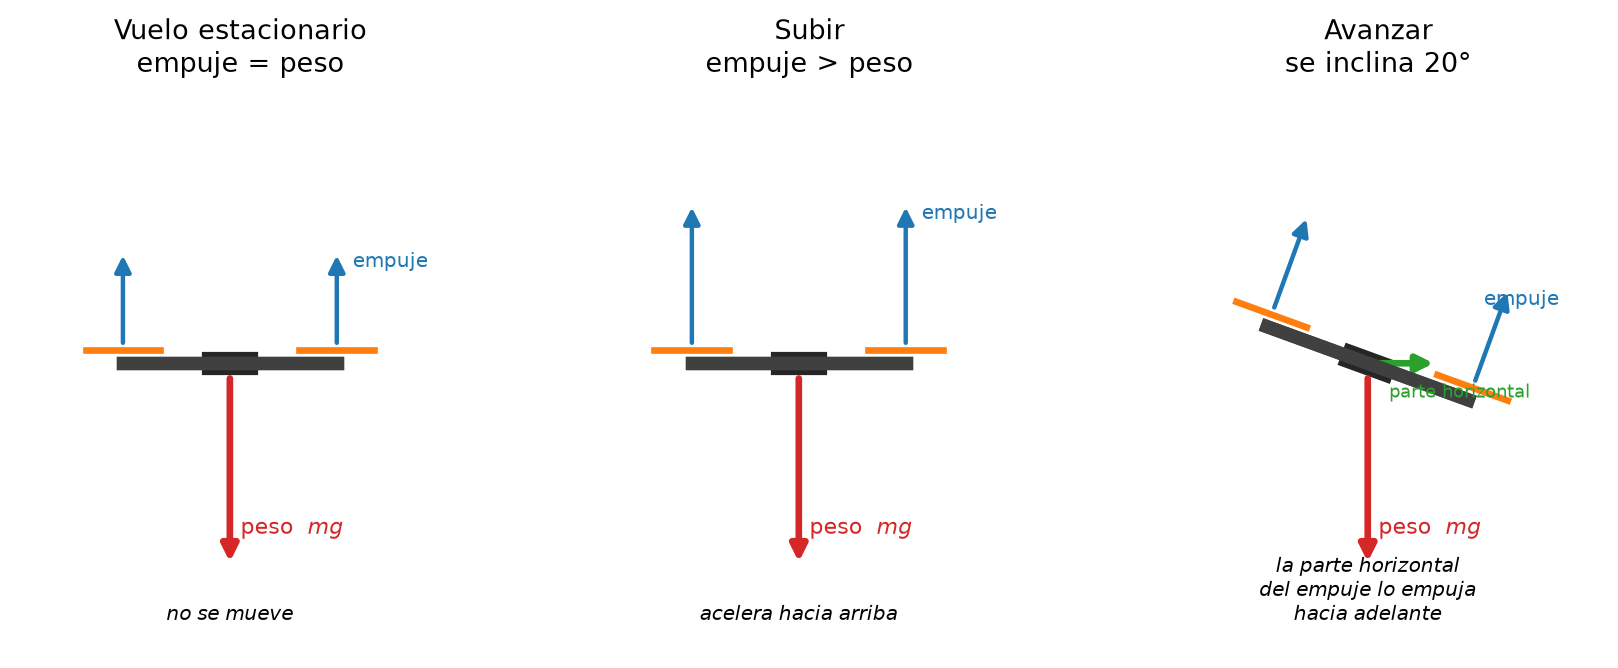
\includegraphics[width=\textwidth]{c_fuerzas.png}
\caption{Las dos fuerzas principales: el empuje de las hélices (azul) y el peso (rojo).}
\label{fig:fuerzas}
\end{figure}

\begin{itemize}
  \item Si el empuje total es igual al peso, el dron se queda quieto en el aire: \textbf{vuelo
        estacionario} (\emph{hover}).
  \item Si es mayor, sube; si es menor, baja.
  \item Para avanzar, el dron \textbf{se inclina}: el empuje ya no apunta hacia arriba, y su parte
        horizontal lo empuja hacia adelante (figura~\ref{fig:fuerzas}, derecha). Un cuadrirrotor no
        tiene ``motor hacia adelante'': avanza inclinándose, como una persona que se inclina para
        empezar a caminar.
\end{itemize}

\begin{ejemplo}
Sostén un libro con la mano extendida, plano. Para moverlo hacia adelante sin empujarlo, inclínalo un
poco: la fuerza de tu mano ``hacia arriba'' ahora tiene una parte hacia adelante. Así avanza un dron.
\end{ejemplo}

\section{Cómo se mueve: subir, alabeo, cabeceo y guiñada}

Un objeto en el espacio puede girar alrededor de tres ejes (figura~\ref{fig:ejes-c}). En aviación
esos giros tienen nombre:
\begin{description}
  \item[Alabeo (roll, $\phi$):] girar alrededor del eje que va al frente; el dron ``se ladea''.
  \item[Cabeceo (pitch, $\theta$):] girar alrededor del eje lateral; ``asiente con la cabeza''.
  \item[Guiñada (yaw, $\psi$):] girar alrededor del eje vertical; cambia hacia dónde mira.
\end{description}

\begin{figure}[H]
\centering
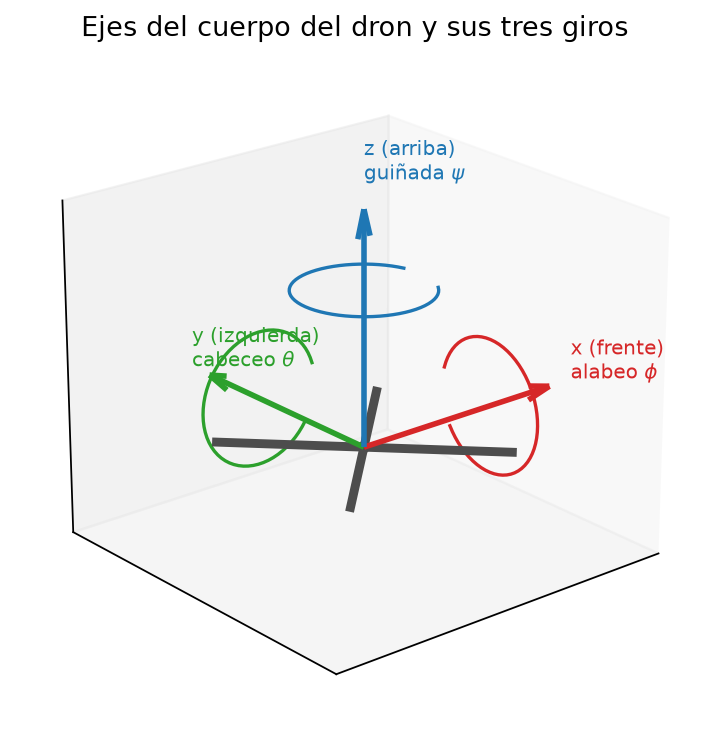
\includegraphics[width=0.6\textwidth]{c_ejes.png}
\caption{Ejes del cuerpo: \emph{x} al frente, \emph{y} a la izquierda, \emph{z} arriba.}
\label{fig:ejes-c}
\end{figure}

Con cuatro motores se controla todo así (figura~\ref{fig:movimientos}):

\begin{figure}[H]
\centering
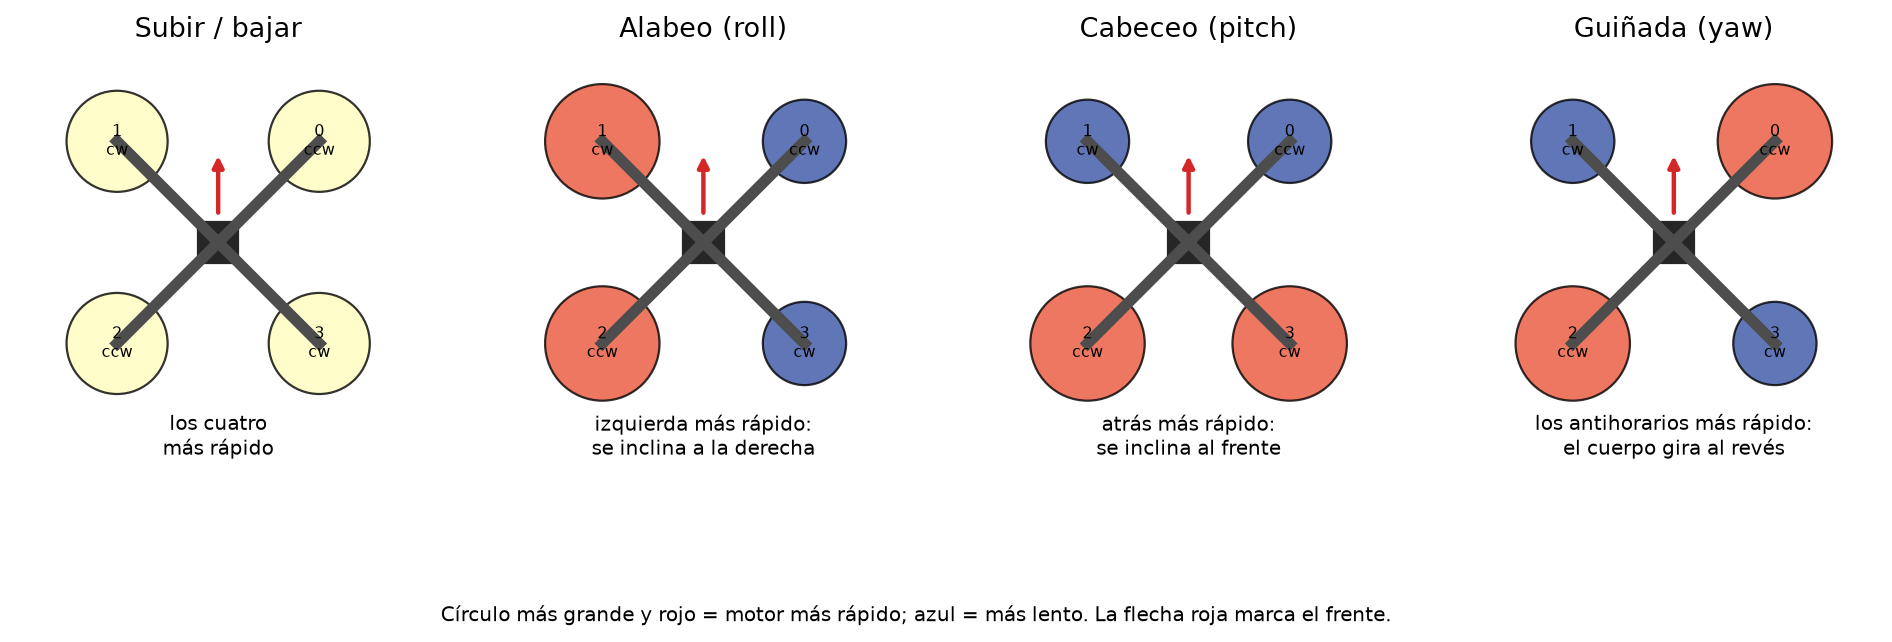
\includegraphics[width=\textwidth]{c_movimientos.png}
\caption{Cómo produce el dron cada movimiento solo cambiando la velocidad de los motores.}
\label{fig:movimientos}
\end{figure}

\begin{itemize}
  \item \textbf{Subir o bajar:} los cuatro motores aceleran o frenan por igual.
  \item \textbf{Alabeo:} los motores de un lado giran más rápido que los del otro; el dron se inclina
        hacia el lado lento y empieza a moverse de lado.
  \item \textbf{Cabeceo:} igual, pero adelante contra atrás; así avanza o retrocede.
  \item \textbf{Guiñada:} aquí entra un truco. Cada hélice, al girar, ``empuja'' el aire de lado y
        el aire, por reacción, intenta hacer girar al dron al revés. Por eso dos hélices giran en un
        sentido y dos en el otro: los efectos se cancelan. Si se aceleran las dos que giran en un
        sentido y se frenan las otras dos, el empuje total no cambia pero sobra par en un sentido, y
        el dron gira sobre sí mismo.
\end{itemize}

\begin{recuerda}
Cuatro motores, cuatro ``perillas'': empuje total, alabeo, cabeceo y guiñada. El avance y el
movimiento lateral no se controlan directamente: se consiguen inclinando el dron. Por eso el control
de un dron es \emph{en cascada}: para ir a una posición hay que pedir una inclinación, y para lograr
la inclinación hay que pedir velocidades a los motores.
\end{recuerda}

\section{Configuración ``+'' y ``X''}

Si un brazo apunta al frente, la configuración es ``+''; si el frente queda entre dos brazos, es
``X''. La ``X'' es la más común: la cámara frontal no ve hélices y los cuatro motores trabajan al
inclinarse hacia adelante. El x500 es ``X''.

\section{El x500}

\begin{figure}[H]
\centering
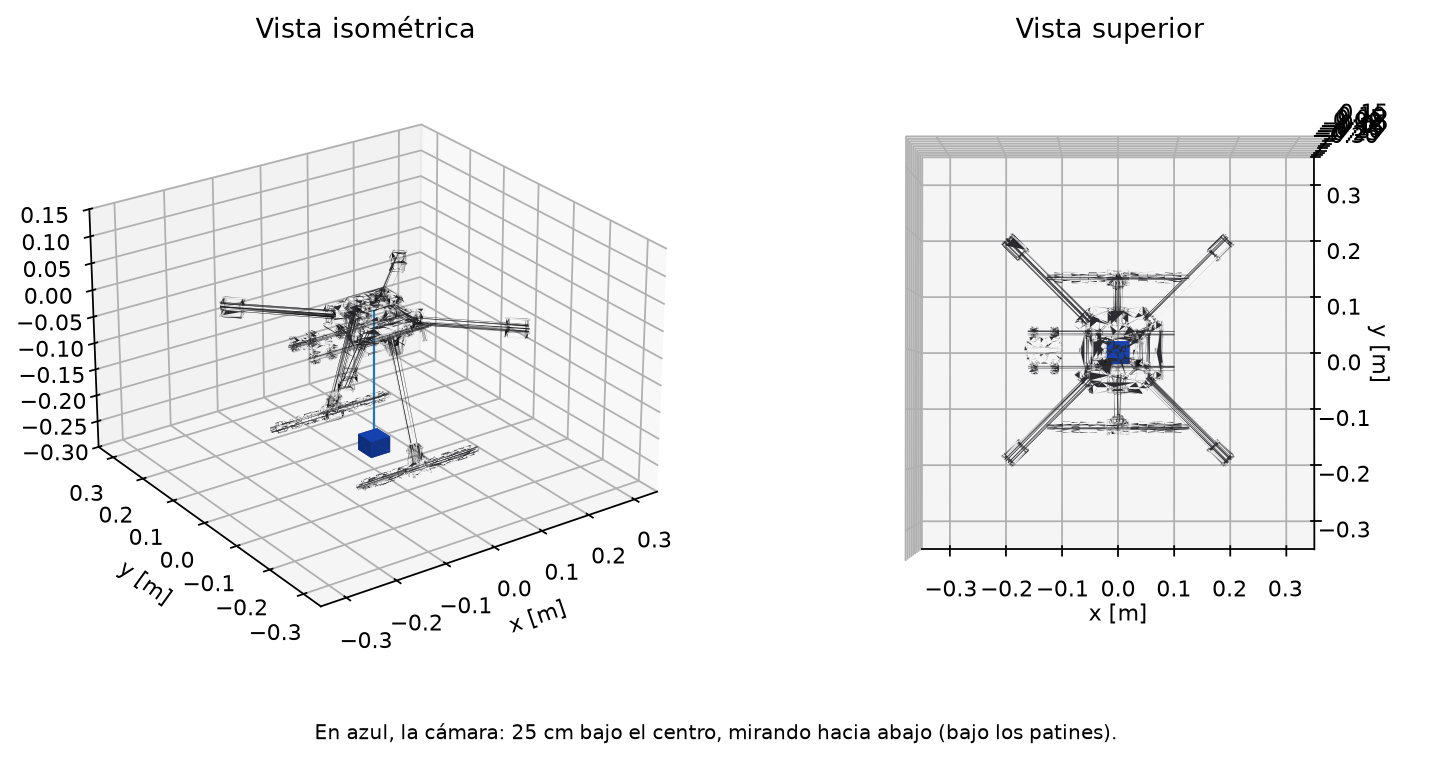
\includegraphics[width=\textwidth]{x500_render.png}
\caption{El x500 de la simulación, dibujado a partir de las mallas de su modelo de PX4.}
\end{figure}

El x500 (Holybro) es el marco de referencia de PX4: barato, robusto y con modelos de simulación
oficiales. El nuestro:
\begin{itemize}
  \item motores a $(\pm0.174, \pm0.174)$~m del centro, en ``X'';
  \item hélices de 13'';
  \item 2.114~kg en total (cuerpo de 2.0~kg, cuatro rotores de 16~g y una cámara de 50~g);
  \item cada motor da hasta 8.55~N; en total $\approx$1.65 veces su peso;
  \item una cámara de $1280\times960$ píxeles con campo horizontal de 1.74~rad (100°) que mira hacia
        abajo, 25~cm debajo del centro (bajo los patines).
\end{itemize}

\begin{tecnico}
En vuelo estacionario cada motor sostiene un cuarto del peso: $2.114\times9.81/4 = 5.18$~N. Con
$f = k_f\omega^2$ y $k_f = 8.54858\times10^{-6}$, la velocidad necesaria es
$\omega = \sqrt{5.18/k_f} = 779$~rad/s, unas 7400 revoluciones por minuto.
\end{tecnico}

\begin{figure}[H]
\centering
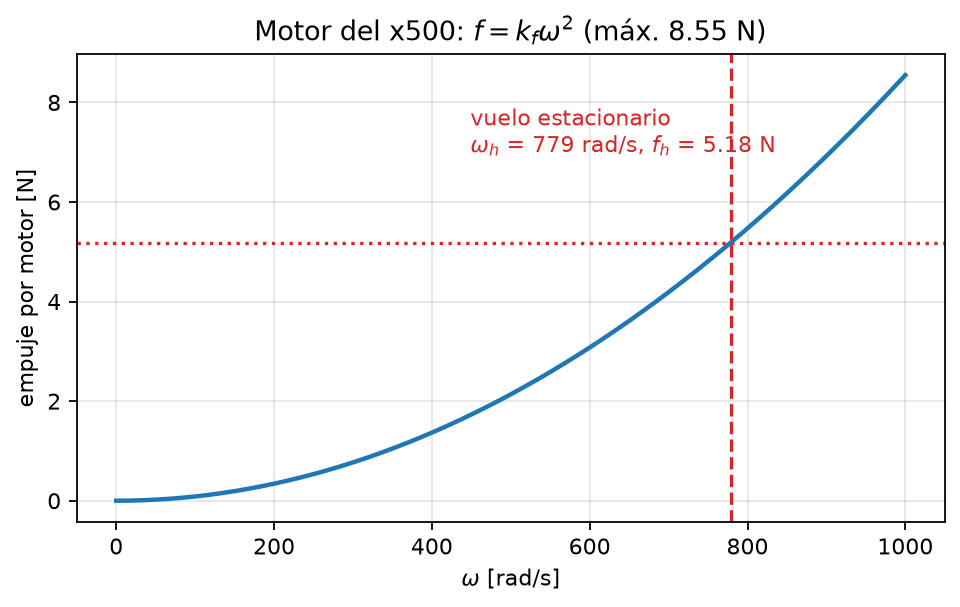
\includegraphics[width=0.7\textwidth]{x500_motor.png}
\caption{Empuje de un motor del x500 contra su velocidad de giro.}
\end{figure}

\section{Para qué sirve un dron en una búsqueda}

Un dron puede recorrer zonas de difícil acceso, ver desde arriba claros que a pie pasarían
desapercibidos, dar las coordenadas exactas de lo que encuentra y repetir la búsqueda las veces que haga
falta. Para hacerlo solo necesita tres capacidades, que son las partes centrales del libro:
\begin{enumerate}
  \item \textbf{percepción y estimación}: reconocer personas y ubicarlas en el mapa (Parte~II);
  \item \textbf{control}: seguir su ruta con precisión aunque haya viento (Parte~III);
  \item \textbf{autonomía}: decidir a dónde ir y cuándo avisar (Parte~V).
\end{enumerate}

\chapter{Física sin miedo}

\begin{enpocas}
Vectores, las leyes de Newton aplicadas al dron, por qué el empuje crece con el cuadrado de la
velocidad, qué es la inercia, qué son los marcos de referencia (ENU, NED, cuerpo) y cómo se describe
una rotación. Al final, las ecuaciones del dron en una página.
\end{enpocas}

\section{Vectores}

Muchas cantidades físicas tienen tamaño y dirección: la velocidad del dron es ``3~m/s \emph{hacia el
este}''. Son \textbf{vectores} y se dibujan como flechas; en tres dimensiones tienen tres componentes,
$v = (v_x, v_y, v_z)$. Posición, velocidad, aceleración, fuerza y velocidad angular son vectores.

\section{Las leyes de Newton aplicadas al dron}

\begin{enumerate}
  \item \textbf{Inercia.} Un cuerpo sigue como está mientras nadie lo empuje: un dron que avanza y deja
        de inclinarse sigue avanzando un rato.
  \item \textbf{$F = ma$.} Para el dron,
        \begin{equation}
        m\,\ddot p = \underbrace{T\,R\,e_3}_{\text{empuje}} \;\underbrace{-\,mg\,e_3}_{\text{peso}} \;+\; \underbrace{d(t)}_{\text{viento}}
        \end{equation}
        con $T$ el empuje total, $R e_3$ la dirección ``arriba'' del dron (cambia si se inclina) y
        $e_3=(0,0,1)$.
  \item \textbf{Acción y reacción.} La hélice empuja aire hacia abajo y el aire la empuja hacia arriba;
        además, al girarla, el motor intenta girar al dron al revés (por eso las hélices van en pares que
        giran en sentidos opuestos).
\end{enumerate}

\section{Empuje: el cuadrado de la velocidad}

El empuje de una hélice es aproximadamente $f = k_f\,\omega^2$. En el Tarot 650, $k_f = 4.24\times
10^{-5}$~N/(rad/s)$^2$ y $\omega_{max} = 680$~rad/s, así que cada motor da hasta 19.6~N. Cada hélice
produce además un par de arrastre $k_m f$ ($k_m = 0.016$~m) que intenta girar al dron.

\begin{recuerda}
Los motores no cambian de velocidad al instante: en el Tarot simulado tienen constantes de tiempo de
0.03~s al acelerar y 0.05~s al frenar (en el x500, 12.5 y 25~ms). Ese retardo, aunque pequeño, limita qué tan agresivo puede ser el control.
\end{recuerda}

\section{Inercia de rotación y par}

Para girar importa el \textbf{momento de inercia} $J$: cuánto se resiste un cuerpo a cambiar su giro.
El Tarot 650 completo (con sus rotores) tiene 0.0341, 0.0361 y 0.0660~kg\,m$^2$ en sus tres ejes. Lo que hace girar es un \textbf{par}
$\tau$, una fuerza aplicada a cierta distancia del centro:
\begin{equation}
J\,\dot\omega = \tau - \omega\times J\omega .
\end{equation}

\begin{leccion}
Un detalle de menos de un milímetro tuvo efectos visibles. La cámara (50~g) tiene su centro de masa a
3~cm del eje y corre el del dron completo 0.7~mm en el x500, el vehículo de las primeras corridas
(0.67~mm en el Tarot). Eso produce un par pequeño pero constante que el controlador
neuronal original no sabía compensar: el dron se quedaba inclinado $\approx$1° y a $\approx$0.2~m del
punto deseado (capítulo~\ref{cap:control-neuronal}).
\end{leccion}

\section{Marcos de referencia: ¿desde dónde mido?}

\begin{description}
  \item[Mundo ENU] (Este, Norte, Arriba): fijo al suelo, con origen en el centro del bosque. Lo usan
        Gazebo y ROS.
  \item[Mundo NED] (Norte, Este, Abajo): el mismo lugar con otros ejes. Lo usan PX4 y ArduPilot.
  \item[Cuerpo:] pegado al dron. En ROS: FLU (frente, izquierda, arriba); en PX4: FRD (frente,
        derecha, abajo).
  \item[Cámara:] eje óptico hacia abajo, ``derecha'' y ``abajo'' de la imagen.
\end{description}

\begin{figure}[H]
\centering
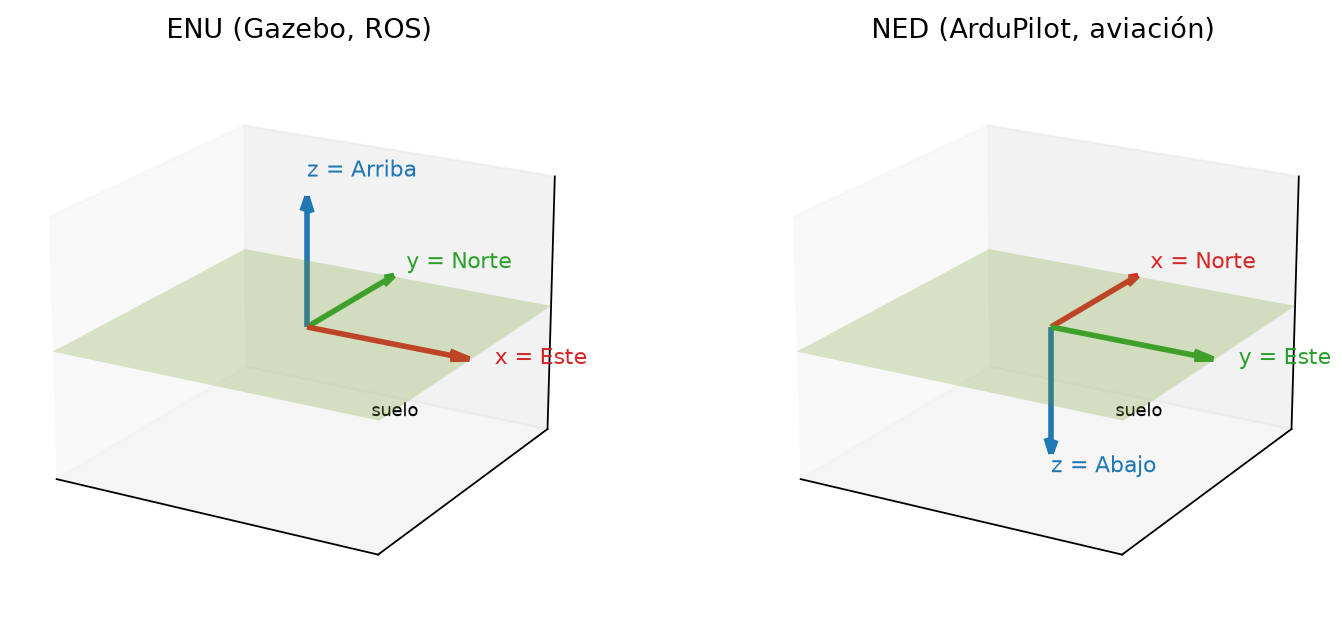
\includegraphics[width=0.9\textwidth]{c_marcos.png}
\caption{ENU y NED. Pasar de uno al otro es intercambiar $x$ con $y$ y cambiar el signo de $z$.}
\end{figure}

\begin{aviso}
Confundir marcos es la causa de error número uno en drones. En este proyecto conviven cinco (ENU, NED,
FLU, FRD y cámara). Cada conversión está en una función con nombre (\cod{ned_a_enu},
\cod{R_enu_flu}, \cod{R_BC}...) y probada en \cod{test/test_mision.py}.
\end{aviso}

\section{Rotaciones}

La orientación se describe con tres ángulos (alabeo $\phi$, cabeceo $\theta$, guiñada $\psi$) o con una
\textbf{matriz de rotación} $R$, cuyas columnas son los ejes del dron vistos desde el mundo; PX4 la
entrega como un \textbf{cuaternión} (cuatro números sin singularidades). En el localizador,
$R = R_z(\psi)R_y(\theta)R_x(\phi)$.

\begin{figure}[H]
\centering
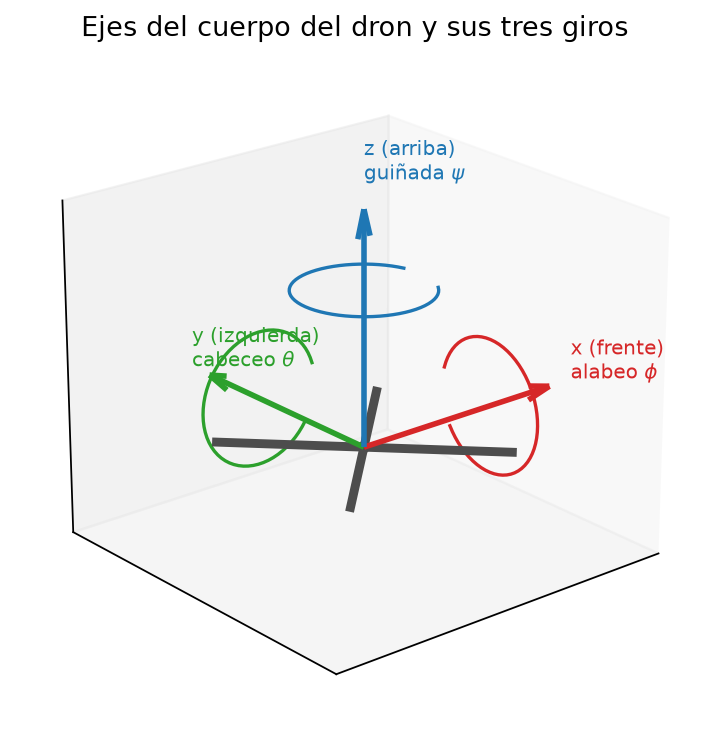
\includegraphics[width=0.55\textwidth]{c_ejes.png}
\caption{Ejes del cuerpo y sus tres giros.}
\end{figure}

\section{Las ecuaciones del dron en una página}

\begin{tcolorbox}[colback=white,colframe=NavyBlue!60!black,title=Modelo del cuadrirrotor]
\begin{align*}
\text{posición:}\quad & m\ddot p = T R e_3 - mg\,e_3 + d(t)\\
\text{orientación:}\quad & \dot R = R\hat\omega\\
\text{giro:}\quad & J\dot\omega = \tau - \omega\times J\omega\\
\text{motores:}\quad & f_i = k_f\omega_i^2,\quad \begin{bmatrix}T\\\tau\end{bmatrix} = A\,f,\quad
A = \begin{bmatrix}1&1&1&1\\ y_i & \cdots\\ -x_i & \cdots\\ -s_ik_m&\cdots\end{bmatrix}
\end{align*}
\end{tcolorbox}

\cod{codigo/sim_modelo.py} simula este modelo con el control base y reproduce las cifras del diseño
original del proyecto. Ese programa usa los parámetros del \textbf{x500} de PX4 (2.0~kg,
$k_f = 8.54858\times10^{-6}$, $\omega_{max} = 1000$~rad/s), no los del Tarot: las cifras y la figura
siguientes son del x500.

\begin{figure}[H]
\centering
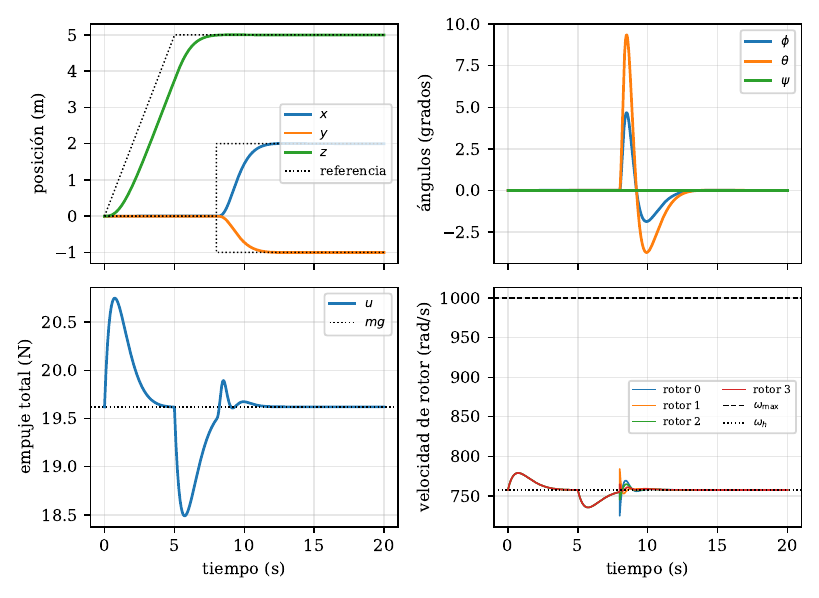
\includegraphics[width=0.85\textwidth]{manual_sim_modelo.png}
\caption{Salida de \cod{sim_modelo.py}: respuesta del modelo del x500 con el control base.}
\end{figure}

\chapter{¿Qué es una simulación? Gazebo y SITL}
\label{cap:simulacion}

\begin{enpocas}
Por qué se simula, qué hace Gazebo, cómo se describe un robot, qué son los plugins, el tiempo simulado
y qué significa que PX4 corra ``en el lazo'' (SITL).
\end{enpocas}

\section{¿Por qué simular?}

Una búsqueda real necesita un dron, un bosque, voluntarios que hagan de personas perdidas y permisos; y
un error de programación puede estrellar el dron. En simulación:
\begin{itemize}
  \item los choques no cuestan nada;
  \item se repite exactamente el mismo bosque, con las mismas personas y el mismo viento, para comparar
        dos estrategias en igualdad de condiciones (imposible al aire libre);
  \item se conoce la verdad: dónde está cada persona, para medir el error de localización;
  \item se pueden correr cientos de vuelos sin supervisión (capítulo~\ref{cap:experimental}).
\end{itemize}

\begin{recuerda}
La simulación no reemplaza el vuelo real: lo prepara y permite responder preguntas que en campo
costarían meses.
\end{recuerda}

\section{Gazebo}

\textbf{Gazebo Harmonic} calcula en cada paso la física (motor DART), dibuja la escena (OGRE~2), genera
las lecturas de los sensores (cámara, IMU, GPS, LiDAR) y ejecuta \emph{plugins}: los motores, el
viento (\cod{WindEffects}), el piloto de ArduPilot o el selector de motores del proyecto.

\begin{figure}[H]
\centering
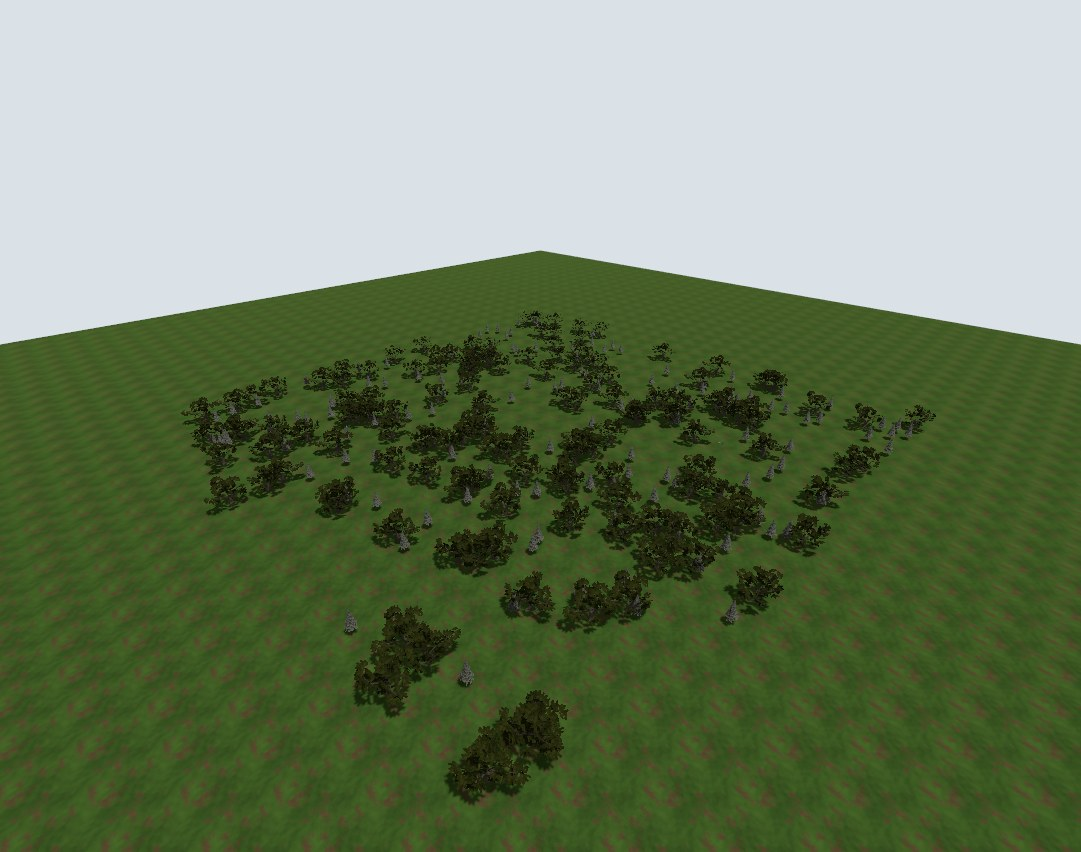
\includegraphics[width=0.75\textwidth]{gz_bosque_aereo.jpg}
\caption{El bosque de la simulación (oclusión media) visto desde lejos.}
\end{figure}

\section{SDF: cómo se describe un robot}

Robots y mundos se escriben en \textbf{SDF} (XML): eslabones con masa, inercia, forma visual y forma de
colisión; articulaciones; sensores; plugins. El x500 del proyecto es el de PX4 con tres cambios
(capítulo~\ref{cap:x500}): la cámara bajo los patines, viento habilitado y un LiDAR.

\section{Personas con etiqueta}

Gazebo puede asignar una \textbf{etiqueta} a cada modelo (sistema \cod{Label}). Las personas llevan la
etiqueta~1. Una cámara especial de Gazebo (\emph{boundingbox camera}) devuelve entonces el recuadro de
la parte \emph{visible} de cada persona: así se etiquetaron solas las 3000 imágenes del dataset del
detector (capítulo~\ref{cap:detector}).

\section{Tiempo simulado}

La simulación tiene su propio reloj: si la computadora es lenta, todo va más despacio pero los resultados
no cambian. El \textbf{factor de tiempo real} mide la proporción. Todos los nodos usan el reloj de
Gazebo (\cod{use_sim_time}).

\section{SITL: el piloto real en la computadora}

En \textbf{SITL} (\emph{software in the loop}) el mismo programa del piloto automático que volaría en
el dron real ---PX4 o ArduCopter--- corre en la computadora y recibe los sensores simulados. Lo que se
prueba aquí es casi lo que volará. El paso siguiente sería HITL: el controlador de vuelo físico
conectado a la simulación.

\begin{leccion}
PX4 trae su propia configuración de Gazebo, que carga un sistema de video (\cod{GstCameraSystem}). Si
el codificador se atora, acumula cuadros de la cámara: llegó a 110~MB/s, 23~GB en minutos, y el sistema
operativo terminó matando la simulación (y otra que estaba abierta). Ahora el \emph{launch} abre Gazebo
sin esa configuración y conecta PX4 a ese Gazebo (\cod{PX4_GZ_STANDALONE}).
\end{leccion}

\chapter{ROS 2 y PX4 para principiantes}

\begin{enpocas}
La terminal en cinco minutos, qué es ROS~2 (nodos, tópicos, mensajes, parámetros, launch), qué es PX4,
y cómo se hablan los dos por medio del agente uXRCE-DDS.
\end{enpocas}

\section{La terminal en cinco minutos}

\begin{lstlisting}[style=bash]
pwd                      # ¿en qué carpeta estoy?
ls                       # ¿qué hay aquí?
cd ~/ros2_ws             # entrar a una carpeta
cat archivo.txt          # ver un archivo
Ctrl+C                   # detener el programa que está corriendo
\end{lstlisting}

\begin{consejo}
Tab completa nombres y la flecha arriba recupera la orden anterior.
\end{consejo}

\section{ROS 2}

\textbf{ROS~2} (\emph{Robot Operating System}) conecta muchos programas pequeños. Cada programa es un
\textbf{nodo}; los nodos se mandan \textbf{mensajes} por canales con nombre llamados \textbf{tópicos}.
Uno \emph{publica}, otros se \emph{suscriben}, sin conocerse entre sí.

\begin{ejemplo}
Una cocina de restaurante: quien toma pedidos los pega en un tablero (tópico), el cocinero los toma
de ahí y deja los platos en la barra (otro tópico), de donde los recoge el mesero. Nadie habla con
nadie directamente.
\end{ejemplo}

En este proyecto:
\begin{longtable}{>{\raggedright\arraybackslash}p{4.5cm}p{10.5cm}}
\toprule
\textbf{Tópico} & \textbf{Qué lleva} \\ \midrule \endhead
\cod{/camera} & imágenes de la cámara del dron (Gazebo $\rightarrow$ ROS) \\
\cod{/detecciones} & recuadros de personas que encuentra YOLO \\
\cod{/personas/estimaciones} & una posición en el suelo por cada detección \\
\cod{/personas/candidatas} & candidatas fusionadas con su confianza y número de detecciones \\
\cod{/personas/gps}, \cod{/personas/alerta} & aviso de cada persona confirmada \\
\cod{/fmu/out/vehicle_odometry} & posición y orientación estimadas por PX4 \\
\cod{/fmu/in/trajectory_setpoint} & consigna de posición que manda la misión a PX4 \\
\cod{/x500/lidar/points} & nube de puntos del LiDAR \\
\bottomrule
\end{longtable}

\begin{lstlisting}[style=bash]
ros2 node list
ros2 topic list
ros2 topic echo /personas/alerta
ros2 topic hz /camera
\end{lstlisting}

Los ajustes de cada nodo son \textbf{parámetros}; un archivo \textbf{launch} arranca todos los nodos con
sus parámetros. El nuestro, \cod{simulacion.launch.py}, también genera el bosque y arranca Gazebo,
PX4 o ArduPilot y MAVProxy.

\section{PX4}

\textbf{PX4} es uno de los dos pilotos automáticos de código abierto más usados (el otro es ArduPilot).
Estima el estado con un filtro de Kalman (EKF2), controla en cascada (posición $\rightarrow$
velocidad $\rightarrow$ actitud $\rightarrow$ velocidad angular) y tiene modos de vuelo. Dos son clave
aquí:
\begin{description}
  \item[Offboard:] PX4 obedece consignas de una computadora externa (nuestra misión) que debe llegar
        al menos dos veces por segundo; si dejan de llegar, PX4 se protege.
  \item[Neural Control] (módulo \cod{mc_nn_control}, en la versión 1.17): una red neuronal calcula
        directamente los comandos de los cuatro motores (capítulo~\ref{cap:control-neuronal}).
\end{description}

\section{El puente: uXRCE-DDS}

PX4 tiene su propio sistema interno de mensajes (uORB). El \textbf{agente Micro XRCE-DDS} los traduce a
tópicos de ROS~2 con el prefijo \cod{/fmu/}: \cod{/fmu/out/...} lo que publica PX4,
\cod{/fmu/in/...} lo que recibe. Los tipos de mensaje vienen del paquete \cod{px4_msgs}, que debe ser
de la misma versión que PX4 (\cod{release/1.17}).

\begin{leccion}
En PX4~1.17 algunos mensajes son \emph{versionados}: el estado del vehículo se publica en
\cod{/fmu/out/vehicle_status_v1}, no en \cod{/fmu/out/vehicle_status} como decía el diseño original.
Escuchar el tópico equivocado no da error: simplemente nunca llega nada.
\end{leccion}

\section{Workspace y compilación}

\begin{lstlisting}[style=bash]
cd ~/ros2_ws
colcon build --symlink-install
source install/setup.bash
\end{lstlisting}
El workspace contiene \cod{mision} (Python), \cod{mision_gz_plugins} (C++), \cod{px4_msgs} y, para
ArduPilot, \cod{ardupilot_gazebo}.


\part{Ver y ubicar: percepción y estimación}
\chapter{Qué es una imagen para una computadora}
\label{cap:imagen}

\begin{enpocas}
Píxeles y canales de color, cómo forma una imagen una cámara, qué es el campo de visión, qué ve una
cámara que apunta hacia abajo, y por qué una persona a 30~m ocupa tan pocos píxeles.
\end{enpocas}

\section{Una imagen es una tabla de números}

La cámara del dron entrega imágenes de 1280 columnas por 960 filas: más de 1.2 millones de
\textbf{píxeles}. Cada píxel tiene tres números entre 0 y 255: cuánto rojo, cuánto verde y cuánto azul
(RGB). Una persona vista desde arriba es un pequeño grupo de píxeles de colores distintos al pasto: la
ropa, la piel, el cabello.

\begin{figure}[H]
\centering
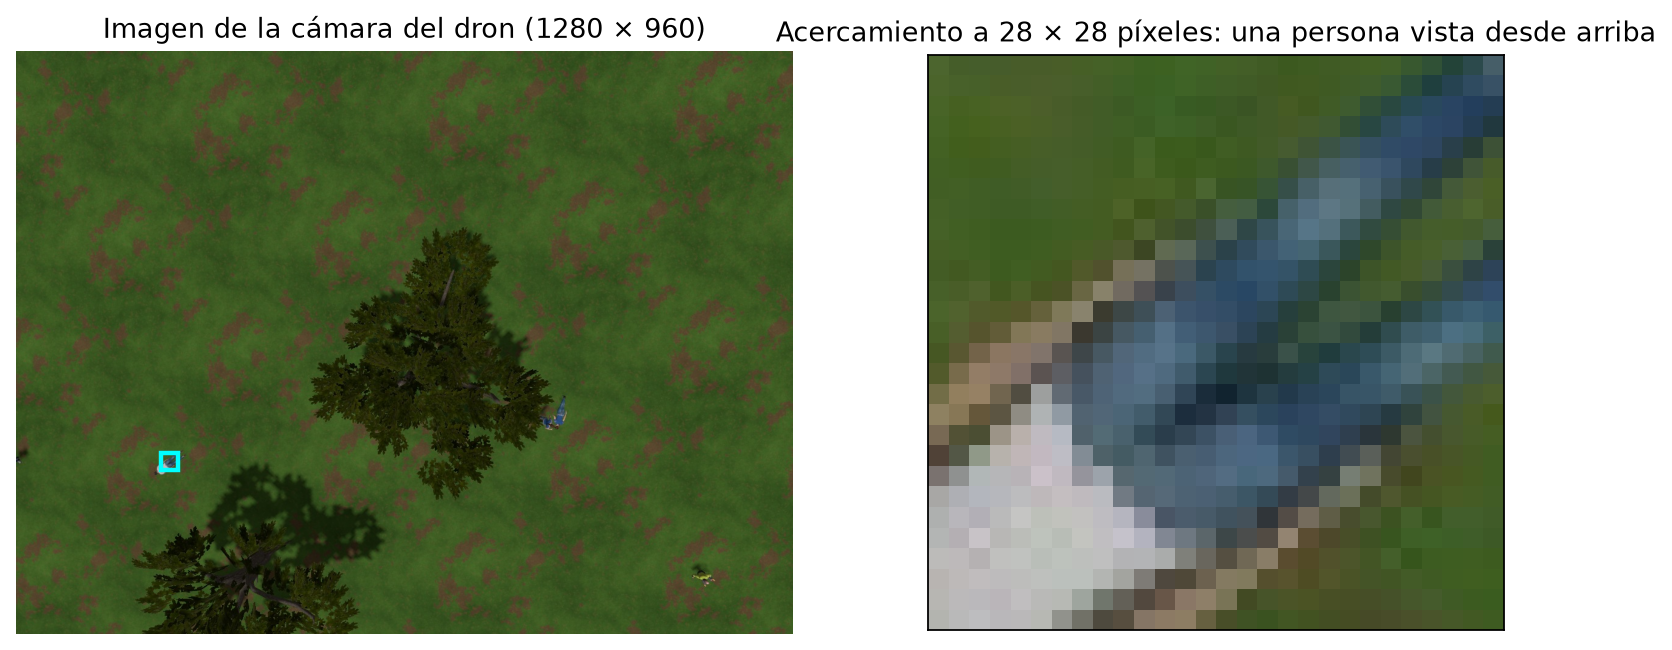
\includegraphics[width=\textwidth]{pixeles_persona.png}
\caption{Una imagen de la cámara del dron y un acercamiento a una de las personas: a 30~m, una persona
apenas ocupa unas decenas de píxeles.}
\end{figure}

\section{Cómo forma una imagen una cámara}

El modelo de \textbf{cámara estenopeica} supone una caja con un agujero: la luz de cada punto entra en
línea recta y llega a un punto del sensor. Un punto a distancia $Z$ y desplazado $X$ aparece en
\begin{equation}
u = f\,\frac{X}{Z},\qquad f = \frac{W/2}{\tan(\text{HFOV}/2)} = \frac{640}{\tan(0.87)} \approx 540\ \text{píxeles}.
\end{equation}
Toda la información de la cámara se resume en la \textbf{matriz intrínseca}
\begin{equation}
K = \begin{bmatrix} f & 0 & W/2\\ 0 & f & H/2\\ 0 & 0 & 1\end{bmatrix},
\end{equation}
que Gazebo publica en \cod{/camera_info}.

\begin{figure}[H]
\centering
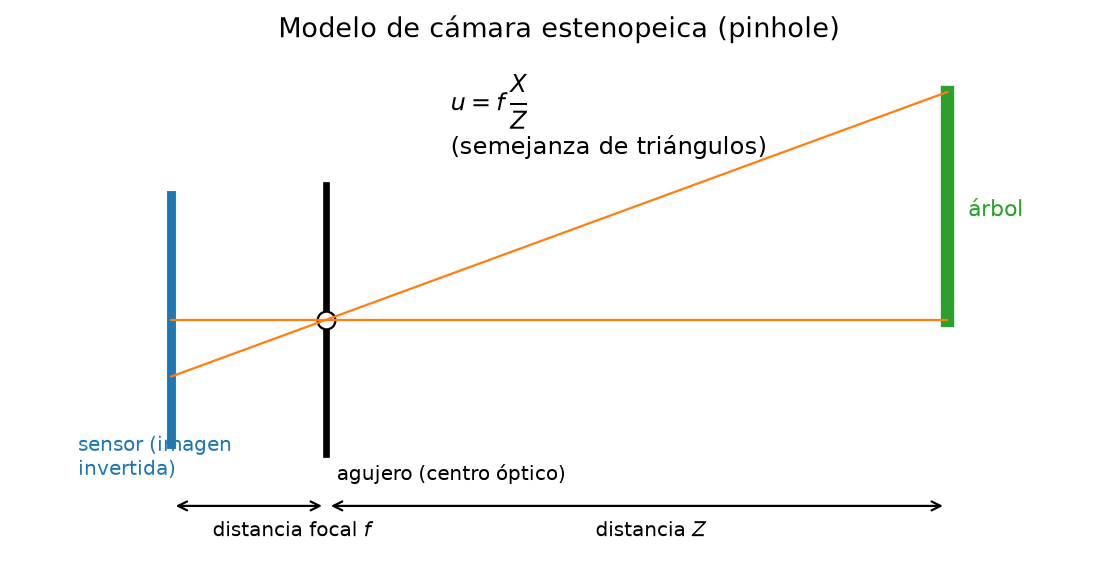
\includegraphics[width=0.8\textwidth]{c_estenopeica.png}
\caption{El modelo estenopeico: la imagen se forma por rayos rectos que pasan por el centro óptico.}
\end{figure}

\section{Una cámara que mira hacia abajo}

La cámara del Tarot 650 (la \cod{mono_cam} de PX4) tiene un campo horizontal de 1.74~rad (100°) y apunta al suelo. A 30~m de altura su
\textbf{huella} en el suelo mide
\begin{equation}
2\cdot30\cdot\tan(0.87) \approx 71\ \text{m}\ \text{de ancho}\quad\times\quad 53\ \text{m de alto}.
\end{equation}
Cada píxel cubre entonces unos $71/1280 \approx 5.5$~cm. Una persona de pie, vista desde arriba
(hombros de unos 45~cm), ocupa $\approx$8 píxeles de ancho; acostada, unos 30 de largo. Por eso hace
falta un detector entrenado para objetos pequeños y por eso la misión baja a 20~m para mirar mejor los
casos dudosos.

\begin{figure}[H]
\centering
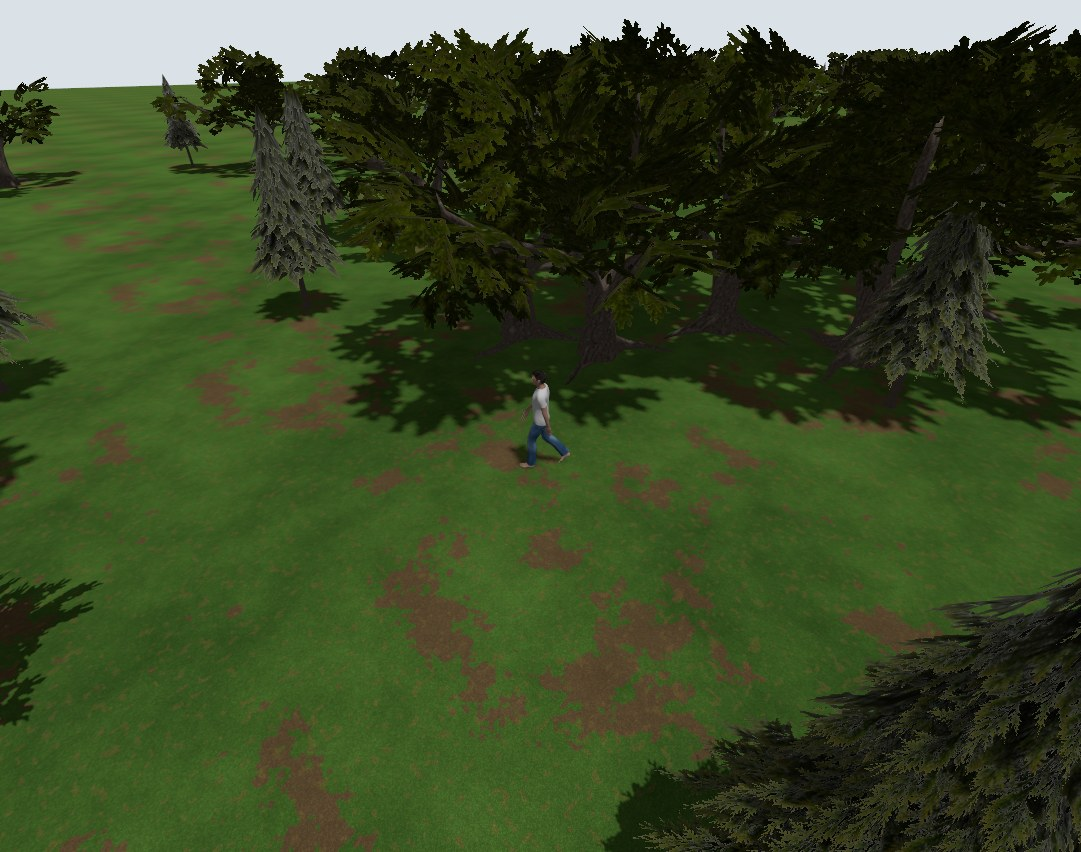
\includegraphics[width=0.49\textwidth]{gz_persona_de_pie.jpg}\hfill
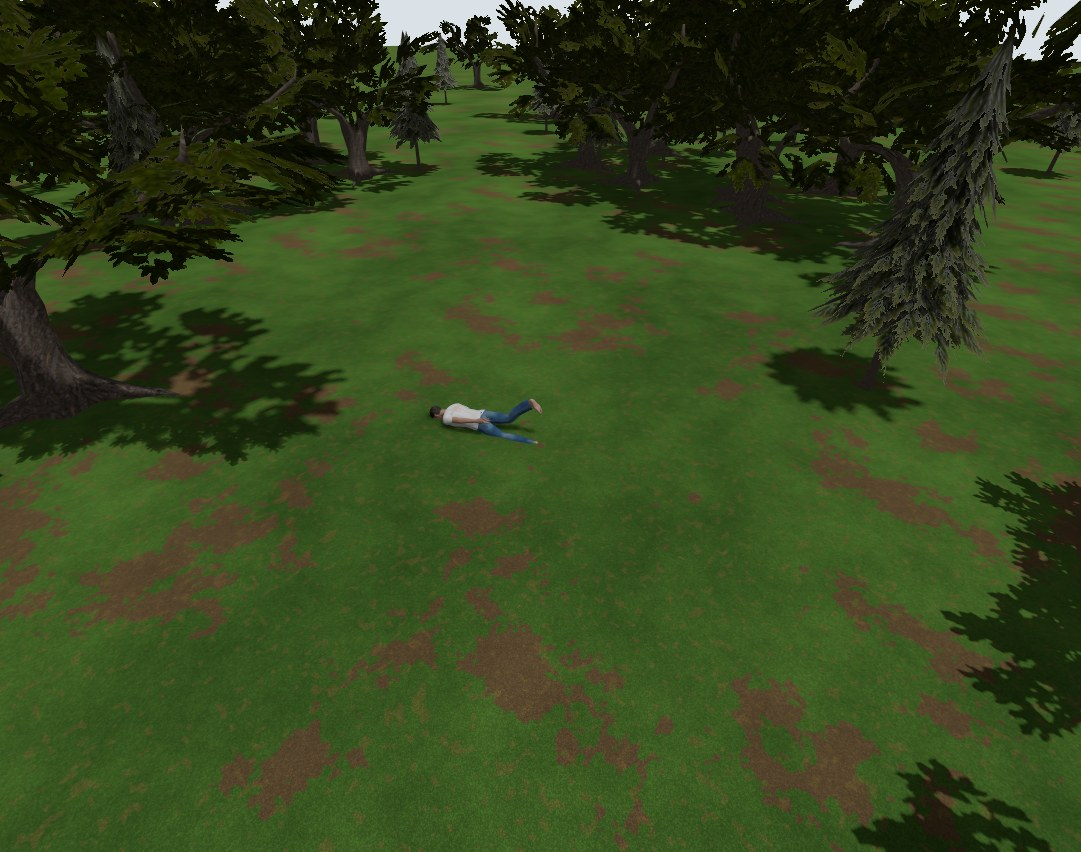
\includegraphics[width=0.49\textwidth]{gz_persona_acostada.jpg}
\caption{Una persona de pie y una acostada en el bosque simulado (vistas oblicuas para el libro; el
dron las ve desde arriba).}
\end{figure}

\section{Del píxel al mundo}

Un píxel no dice a qué distancia está lo que muestra, solo en qué \emph{dirección}: cada píxel es un
\textbf{rayo}. Para ubicar a la persona hay que cortar ese rayo con el suelo; si además se conoce la
incertidumbre de la posición y la orientación del dron, se puede calcular qué tan grande es el error
(capítulo~\ref{cap:localizacion}).

\begin{recuerda}
Una cámara da direcciones, no distancias. Con el suelo plano y la altura del dron, cada dirección se
convierte en un punto del mapa.
\end{recuerda}

\chapter{Redes neuronales y YOLO sin complicaciones}

\begin{enpocas}
Qué es aprender con ejemplos, cómo funciona una neurona, qué es una convolución, cómo detecta objetos
YOLO y cómo se mide si funciona: IoU, precisión, recall y mAP.
\end{enpocas}

\section{Programar contra aprender}

Escribir reglas para reconocer a una persona desde el aire (``un grupo de píxeles de color piel...'')
falla de inmediato: hay ropa de todos colores, sombras, personas acostadas o tapadas por ramas. El
\textbf{aprendizaje automático} hace lo contrario: se le dan miles de imágenes con la respuesta correcta
y el programa ajusta sus parámetros hasta acertar.

\section{La neurona artificial}

Una neurona multiplica cada entrada por un \textbf{peso}, suma todo con un \textbf{sesgo} y pasa el
resultado por una función de activación:
\begin{equation}
y = \text{activación}\Big(\sum_i w_i x_i + b\Big).
\end{equation}
Muchas neuronas en capas forman una \textbf{red}. Entrenar es encontrar los pesos que hacen que la red
acierte. La misma idea sirve para ver (YOLO) y para controlar (la red 15-64-32-4 del
capítulo~\ref{cap:control-neuronal}).

\section{Convoluciones}

Las redes para imágenes usan \textbf{convoluciones}: filtros pequeños que se deslizan por la imagen
buscando patrones locales (bordes, texturas, formas). Las primeras capas detectan bordes; las
siguientes, partes; las últimas, objetos completos. Los filtros no se diseñan: se aprenden.

\begin{figure}[H]
\centering
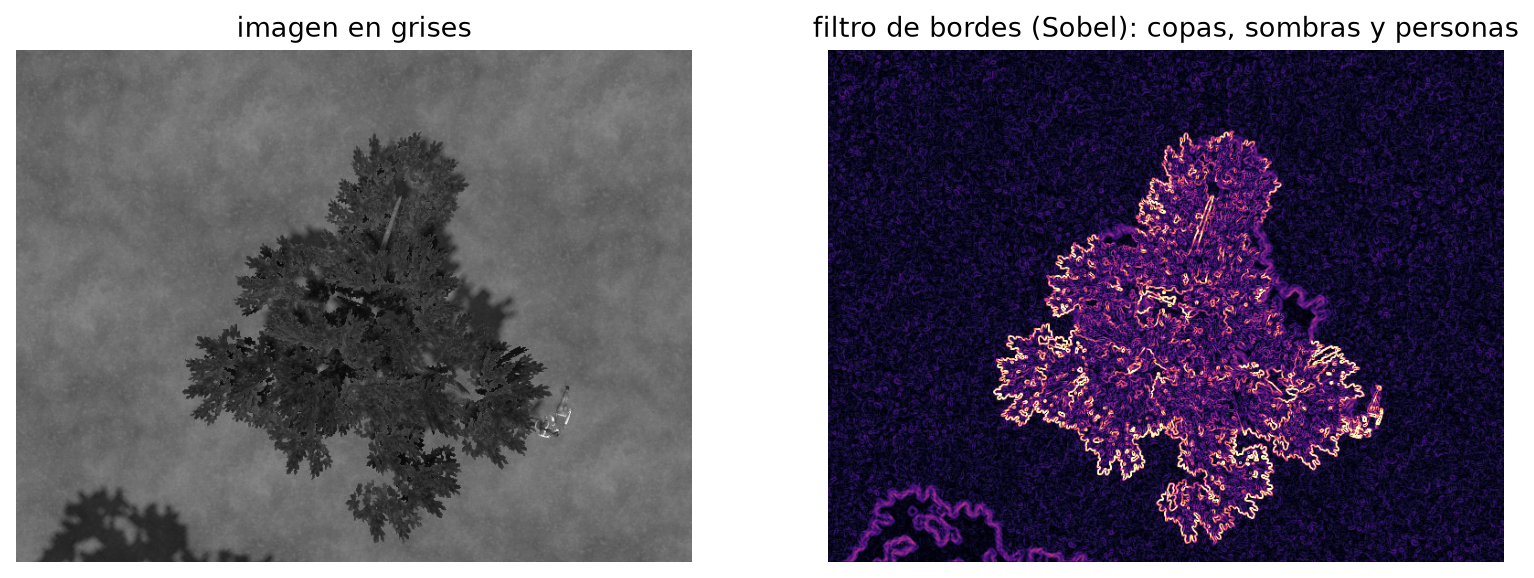
\includegraphics[width=\textwidth]{convolucion_personas.png}
\caption{Un filtro de bordes aplicado a una imagen del dron: resalta copas, sombras y personas.}
\end{figure}

\section{YOLO}

\textbf{YOLO} (\emph{You Only Look Once}) predice en una sola pasada todos los recuadros de la imagen,
cada uno con su clase y su confianza. Usamos \textbf{YOLO26s}, la versión vigente de Ultralytics en
tamaño \emph{small}: la \emph{nano} es más rápida pero pierde personas pequeñas. Procesa una imagen de
1280 píxeles en $\approx$16~ms en la GPU.

\begin{figure}[H]
\centering
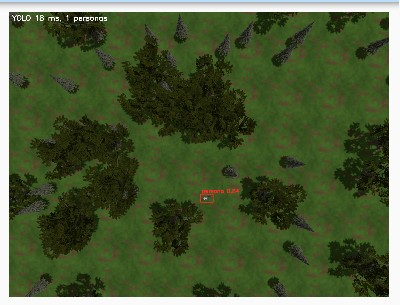
\includegraphics[width=0.55\textwidth]{panel_yolo_personas.jpg}
\caption{Lo que entrega YOLO durante el vuelo: el recuadro rojo con la clase ``persona'' y su
confianza.}
\end{figure}

\section{Cómo se mide si funciona}

\begin{figure}[H]
\centering
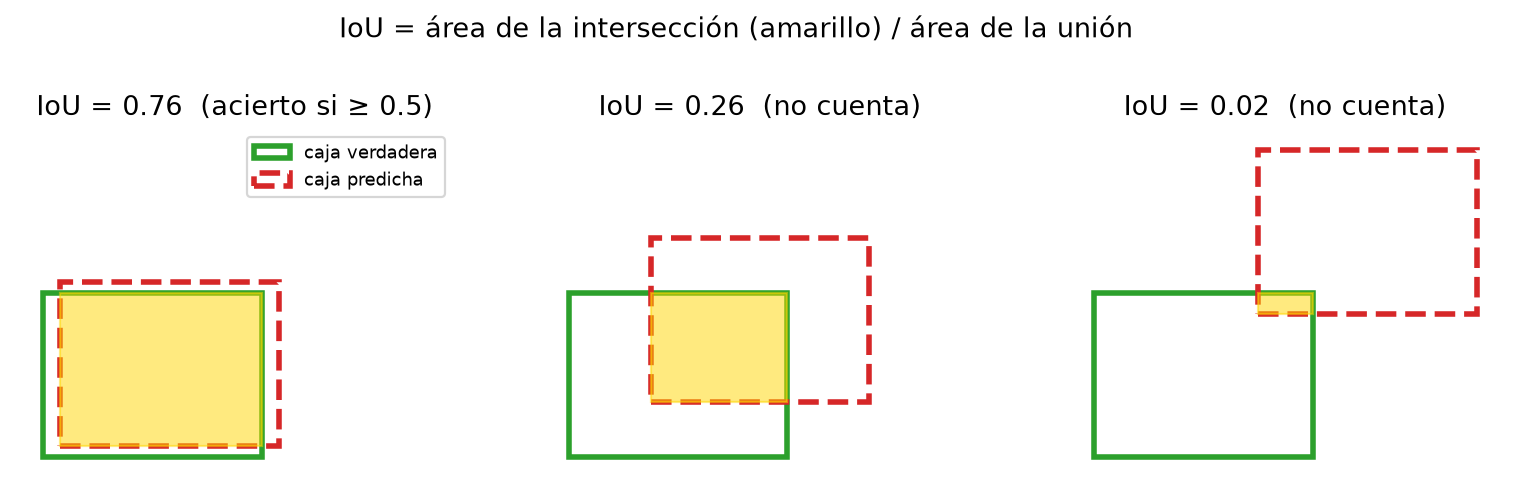
\includegraphics[width=\textwidth]{c_iou.png}
\caption{IoU: intersección sobre unión de la caja predicha y la verdadera.}
\end{figure}

\begin{description}
  \item[Verdadero positivo:] dijo ``persona'' y había una (con IoU $\ge$ 0.5).
  \item[Falso positivo:] dijo ``persona'' y no había (por ejemplo, la sombra de un roble).
  \item[Falso negativo:] había una persona y no la vio.
\end{description}
\begin{align}
\text{precisión} &= \frac{VP}{VP + FP} && \text{(cuando dice ``persona'', ¿cuántas veces acierta?)}\\
\text{recall} &= \frac{VP}{VP + FN} && \text{(de las personas que hay, ¿cuántas encuentra?)}
\end{align}
La \textbf{mAP50} resume la curva precisión-recall con IoU $\ge$ 0.5; la \textbf{mAP50-95} exige además
cajas más ajustadas.

\begin{ejemplo}
En una búsqueda, perder a una persona (falso negativo) es mucho peor que revisar una sombra (falso
positivo). Por eso el umbral de confianza del detector es bajo (0.25) y la misión decide después,
juntando varias detecciones, qué candidatas son confiables.
\end{ejemplo}

\chapter{El detector de personas}
\label{cap:detector}

\begin{enpocas}
Cómo se generó un dataset de 3000 imágenes etiquetadas sin dibujar un solo recuadro a mano, cómo se
entrenó YOLO26s, qué tan bien quedó en cada condición y cómo funciona el nodo detector durante el
vuelo.
\end{enpocas}

\section{Etiquetas automáticas}

\cod{scripts/capturar_dataset.py} genera bosques con distintos niveles de oclusión e iluminación, cada
uno con 30 personas, y coloca dos cámaras con la misma óptica que la del dron ($1280\times960$, 1.74~rad,
hacia abajo): una normal y una \textbf{cámara de cajas} de Gazebo, que entrega el recuadro de la parte
\emph{visible} de cada objeto con etiqueta. Mueve las cámaras a poses al azar de un dron buscando
(entre 12 y 45~m de altura, un poco inclinadas, cualquier orientación) y guarda la imagen y sus cajas.
Una persona tapada por una copa sale recortada o no sale: exactamente lo que el detector puede ver.

\begin{lstlisting}[style=bash]
python3 scripts/capturar_dataset.py ~/datasets/personas_bosque 3000
\end{lstlisting}

Resultado: 3000 imágenes con 13\,202 personas, y un archivo \cod{estratos.csv} con la oclusión, la
iluminación y la altura de cada imagen.

\begin{figure}[H]
\centering
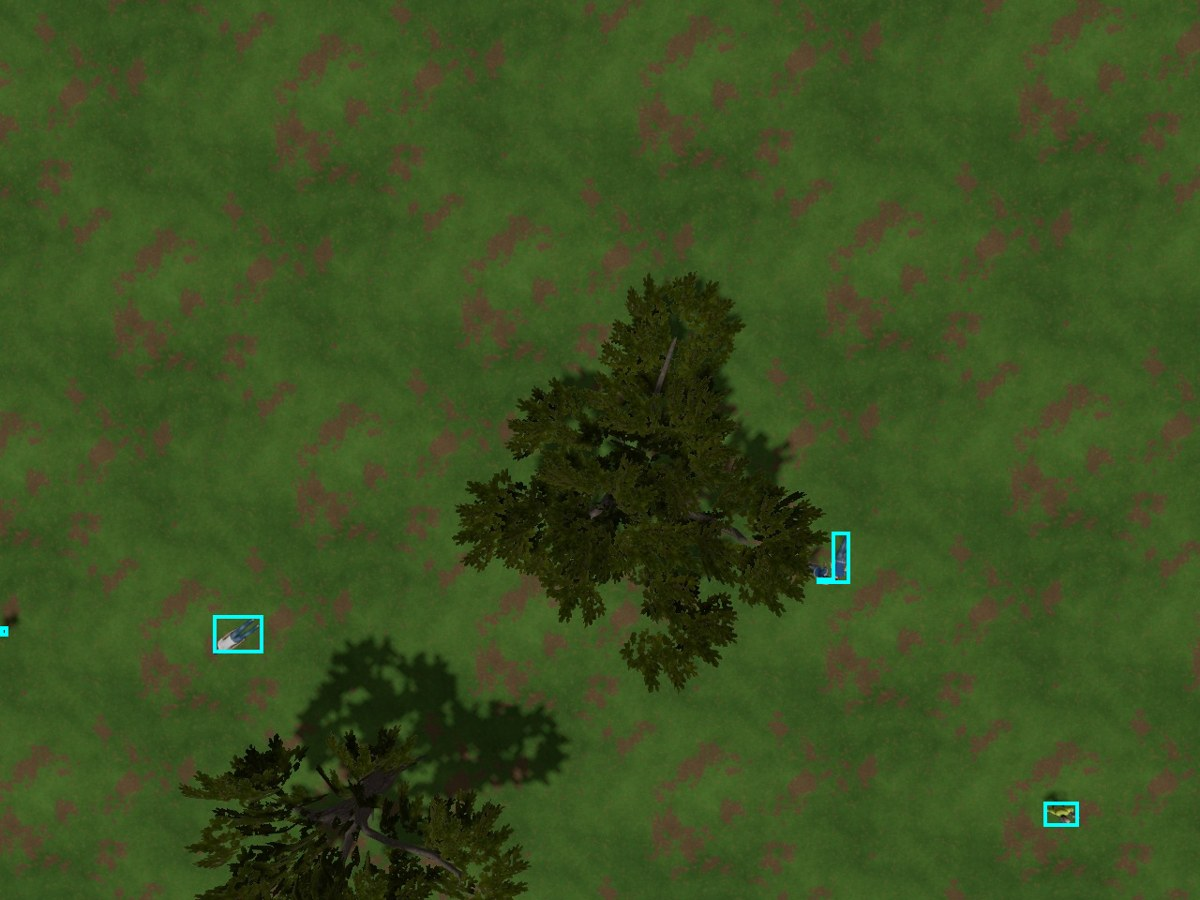
\includegraphics[width=0.8\textwidth]{dataset_etiquetas.jpg}
\caption{Una imagen del dataset con sus etiquetas automáticas (recuadros cian).}
\end{figure}

\section{Entrenamiento}

\begin{lstlisting}[style=bash]
~/.venvs/yolo/bin/python scripts/entrenar_detector.py entrenar --datos ~/datasets/personas_bosque/datos.yaml --epocas 80
\end{lstlisting}

Se parte de los pesos de YOLO26s preentrenados en COCO y se ajusta con imágenes de 1280 píxeles (sin
reducir: las personas son pequeñas) en la GPU. El mejor modelo se copia a
\cod{yolo/personas_yolo26s.pt}, que es el que usa la misión. Resultado en validación (300 imágenes):
\textbf{AP50 = 0.954}, AP50-95 = 0.692, precisión 0.96, recall 0.92, 15.6~ms por imagen.

\begin{figure}[H]
\centering
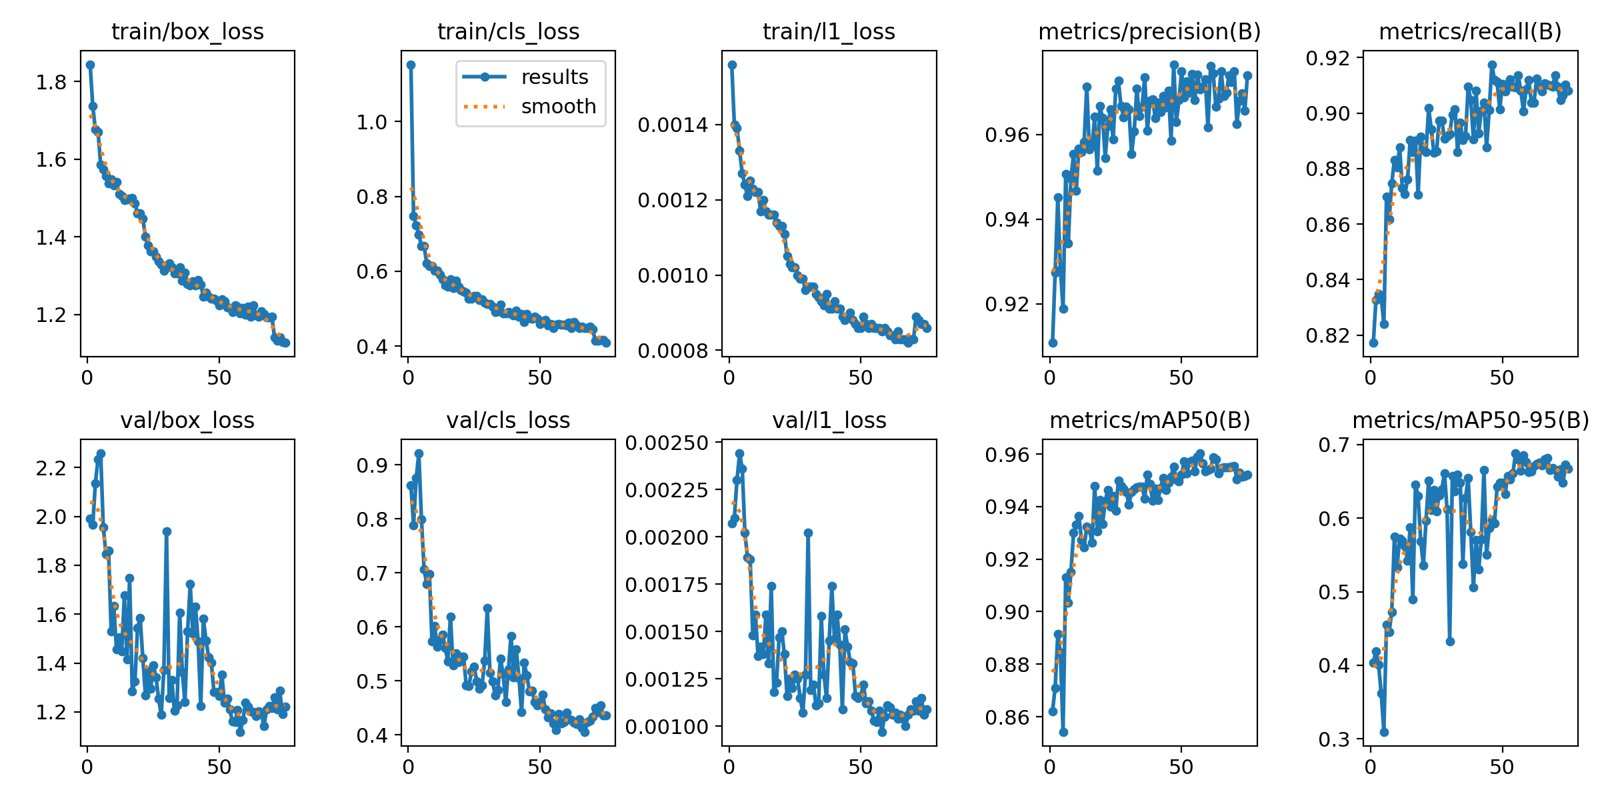
\includegraphics[width=\textwidth]{yolo_p_resultados.jpg}
\caption{Curvas de entrenamiento del detector de personas.}
\end{figure}

\begin{figure}[H]
\centering
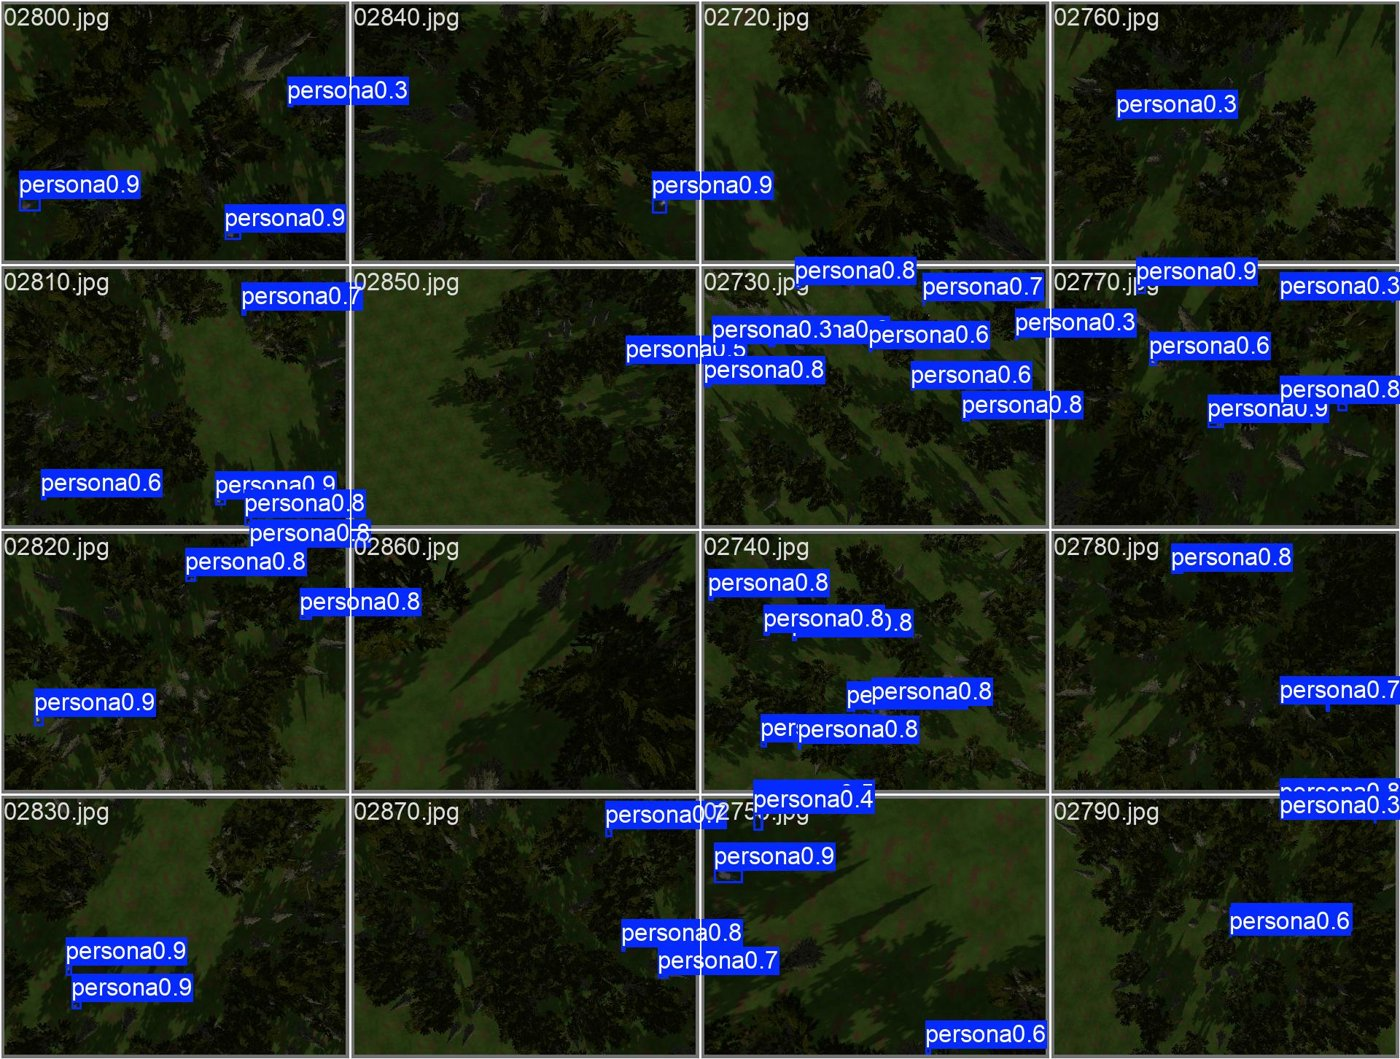
\includegraphics[width=0.85\textwidth]{yolo_p_pred.jpg}
\caption{Predicciones del detector sobre imágenes de validación.}
\end{figure}

\section{Por estrato: dónde falla}

\begin{figure}[H]
\centering
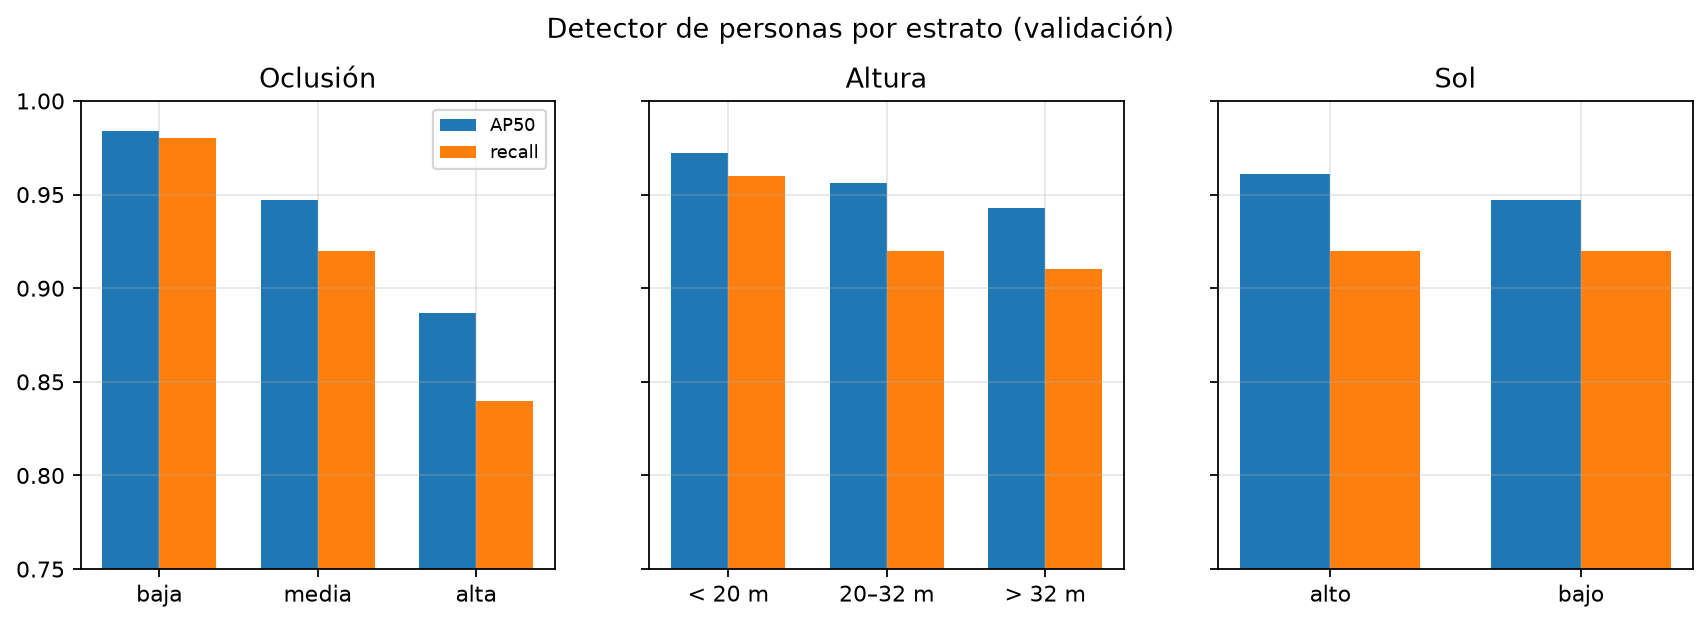
\includegraphics[width=\textwidth]{detector_estratos.png}
\caption{El detector pierde más personas con más copas (recall 0.98 $\rightarrow$ 0.84) y con más
altura; la iluminación casi no importa.}
\end{figure}

\begin{nota}
Con el YOLO26n preentrenado en COCO, sin ajustar, la misión localizó 0 de 3 personas: COCO casi no tiene
personas vistas desde arriba a 30~m. El ajuste con imágenes del simulador es indispensable; para el dron
real habrá que agregar imágenes reales (por ejemplo, el conjunto HERIDAL; \cod{scripts/preparar_datos.py}
las convierte).
\end{nota}

\section{El nodo detector}

\cod{mision/detector_node.py} corre con el Python de \cod{~/.venvs/yolo}, lee \cod{/camera}, aplica el
modelo y publica las cajas en \cod{/detecciones} (con la marca de tiempo de la imagen) y la imagen
anotada en \cod{/camera_yolo}, que Gazebo muestra en el panel ``Detección de personas''. Para estudiar
qué pasa si el detector es más lento (por ejemplo en una computadora a bordo), se le puede agregar
latencia (\cod{latencia_extra_ms}) o hacer que salte cuadros (\cod{saltar_cuadros}).

\chapter{Ubicar a la persona: localización y fusión}
\label{cap:localizacion}

\begin{enpocas}
Cómo se convierte un recuadro de la imagen en un punto del suelo, de dónde viene el error y cómo se
calcula su tamaño (propagación de covarianza), y cómo se juntan muchas detecciones de la misma persona
en una sola candidata cada vez más precisa y confiable.
\end{enpocas}

\section{Del recuadro al suelo: el rayo}

Para cada detección se toma el centro del recuadro $(u,v)$ ---con la cámara hacia abajo, la persona se
ve casi desde arriba y el centro es el mejor punto de apoyo---. Su dirección en el marco de la cámara es
$K^{-1}(u, v, 1)^\top$; se pasa al mundo con la orientación de la cámara ($R_{BC}$, fija respecto al
cuerpo) y la del dron ($R$, que estima PX4):
\begin{equation}
r = R\,R_{BC}\,K^{-1}\begin{bmatrix}u\\v\\1\end{bmatrix},\qquad p_c = \xi + R\,t_{BC},
\end{equation}
donde $\xi$ es la posición del dron y $t_{BC} = (0, 0, -0.25)$~m la de la cámara (bajo los patines).
El punto del suelo ($z = z_t = 0$) es
\begin{equation}
x = p_c + \lambda\,r,\qquad \lambda = \frac{z_t - p_{c,z}}{r_z}.
\end{equation}
Si el rayo no baja ($r_z \ge 0$) no hay intersección; si forma más de 60° con la vertical, el error
sería enorme y se descarta (ver el recuadro de abajo).

\begin{figure}[H]
\centering
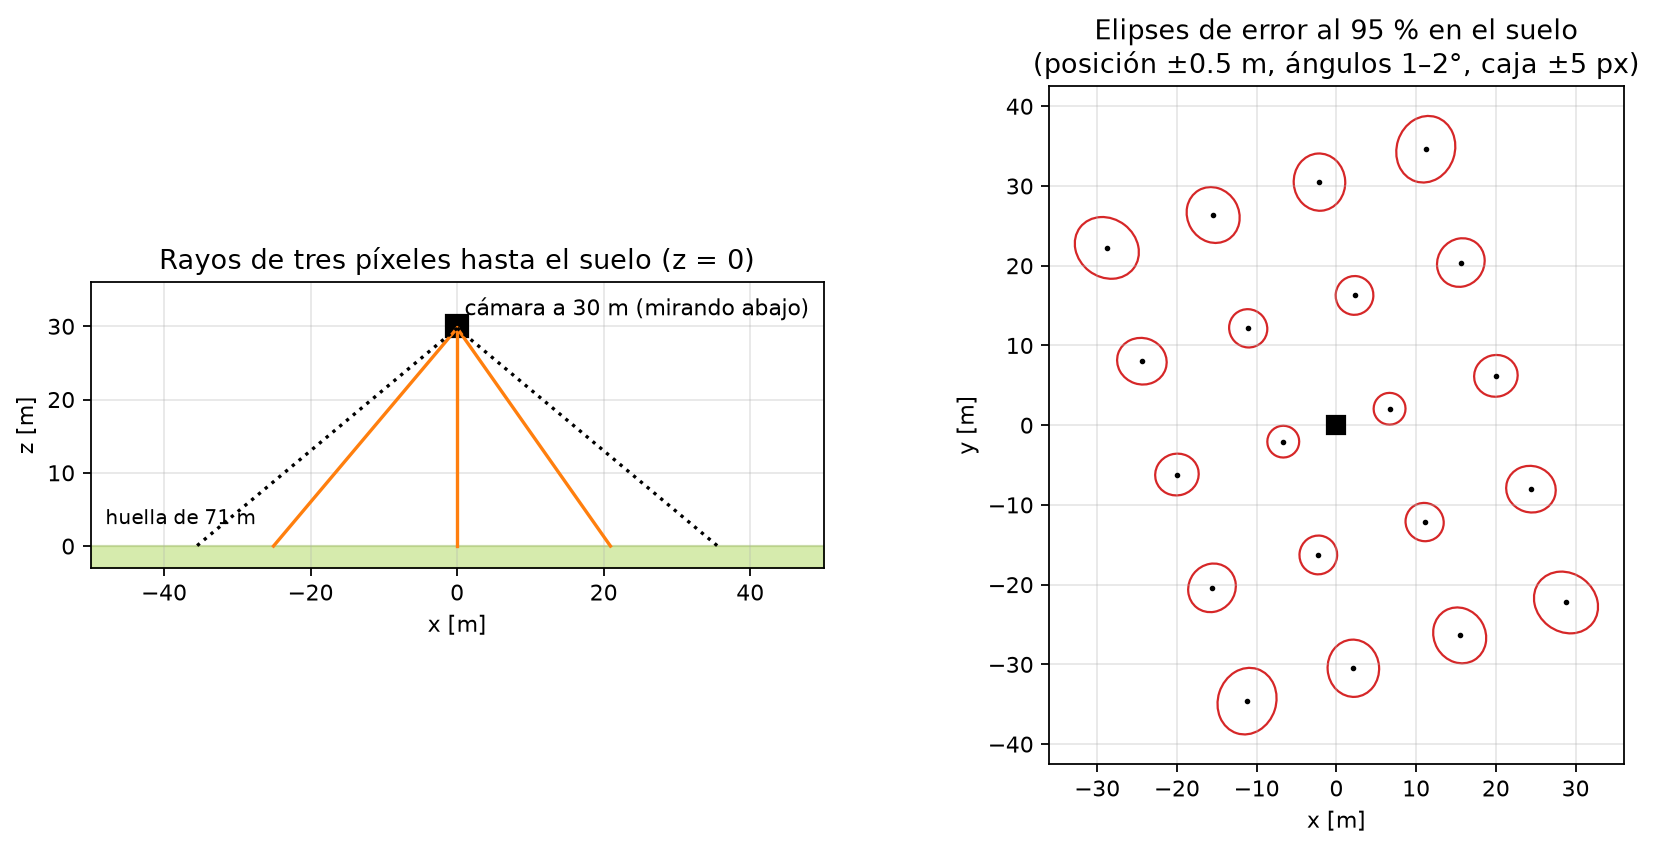
\includegraphics[width=\textwidth]{localizacion.png}
\caption{Izquierda: rayos de tres píxeles hasta el suelo. Derecha: elipses de error al 95~\% para una
rejilla de píxeles, con la incertidumbre típica de PX4.}
\label{fig:localizacion}
\end{figure}

\section{¿Qué tan grande es el error?}

El punto depende de ocho cantidades inciertas: la posición del dron (3), su orientación (3) y el
centro del recuadro (2). Si cada una tiene una varianza conocida ($\Sigma_p$, $\Sigma_\eta$, $\Sigma_u$),
a primer orden la covarianza del punto es
\begin{equation}
\Sigma_x \approx J_p\Sigma_pJ_p^\top + J_\eta\Sigma_\eta J_\eta^\top + J_u\Sigma_uJ_u^\top ,
\end{equation}
con $J$ las derivadas (jacobianos) de $x$ respecto a cada grupo, calculadas numéricamente. La elipse de
la figura~\ref{fig:localizacion} es la representación de $\Sigma_x$. PX4 publica las varianzas de su
estimación en \cod{/fmu/out/vehicle_odometry}, así que el localizador las usa en cada detección.

\begin{ejemplo}
Apuntar con un láser desde un balcón: un pequeño temblor de la mano (orientación) mueve el punto más
cuanto más lejos está el suelo; moverse uno mismo medio metro (posición) mueve el punto medio metro,
esté donde esté. Por eso el error por orientación crece con la altura y el de posición no.
\end{ejemplo}

\cod{codigo/sim_localizacion.py} valida la fórmula con miles de simulaciones al azar (Monte Carlo) y
separa las tres fuentes:

\begin{table}[H]
\centering\small
\begin{tabular}{lccccc}
\toprule
\textbf{Caso} & \textbf{altura} & \textbf{RMSE Monte Carlo} & \textbf{por posición} & \textbf{por orientación} & \textbf{por detección} \\ \midrule
nominal ($\sigma_p$ = 0.5 m, $\sigma_\eta$ = 0.5°, $\sigma_u$ = 5 px) & 20 m & 0.85 m & 0.92 & 0.31 & 0.26 \\
nominal & 30 m & 0.94 m & 0.92 & 0.47 & 0.39 \\
nominal & 40 m & 1.05 m & 0.92 & 0.62 & 0.52 \\
posición degradada ($\sigma_p$ = 2 m) & 30 m & 3.02 m & 3.34 & 0.47 & 0.39 \\
orientación degradada ($\sigma_\eta$ = 2°) & 30 m & 1.81 m & 0.92 & 1.86 & 0.39 \\
detección degradada ($\sigma_u$ = 20 px) & 30 m & 1.78 m & 0.92 & 0.47 & 1.57 \\
\bottomrule
\end{tabular}
\caption{Error de localización y su desglose (salida de \cod{sim_localizacion.py}; las tres últimas
columnas son la contribución lineal en metros). Con un GPS normal domina la posición del dron.}
\end{table}

\begin{figure}[H]
\centering
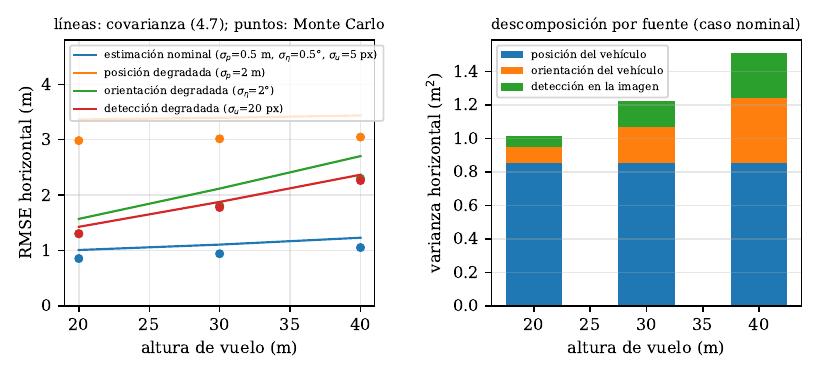
\includegraphics[width=0.85\textwidth]{manual_sim_localizacion.png}
\caption{Figura de \cod{sim_localizacion.py}: la fórmula lineal y el Monte Carlo coinciden.}
\end{figure}

\section{Juntar detecciones: asociación y fusión}

A 3~m/s, una persona queda en la imagen varios segundos y el detector la ve decenas de veces. Cada
detección produce un punto con su elipse. \cod{localizador_node} mantiene una lista de
\textbf{candidatas} y, para cada detección nueva:
\begin{enumerate}
  \item \textbf{Asociación:} calcula su distancia de \textbf{Mahalanobis} a cada candidata,
        \begin{equation}
        d^2 = (x - c)^\top(\Sigma_x + \Sigma_c)^{-1}(x - c),
        \end{equation}
        una distancia ``medida en elipses''. Si la menor es menor que 9.21 (el percentil 99~\% de una
        $\chi^2$ con 2 grados de libertad), es la misma persona; si no, nace una candidata nueva.
  \item \textbf{Fusión:} combina las dos estimaciones pesando cada una por su precisión (fusión de
        información):
        \begin{equation}
        \Sigma_c' = \big(\Sigma_c^{-1} + \Sigma_x^{-1}\big)^{-1},\qquad
        c' = \Sigma_c'\big(\Sigma_c^{-1}c + \Sigma_x^{-1}x\big).
        \end{equation}
        La candidata nueva $c'$ queda más cerca de la estimación más precisa, y su elipse $\Sigma_c'$ es
        siempre más chica que las dos anteriores.
  \item \textbf{Confianza:} acumula la confianza del detector como la probabilidad de que al menos una
        detección sea correcta: $C \leftarrow 1 - (1 - C)(1 - c_i)$.
\end{enumerate}

\begin{figure}[H]
\centering
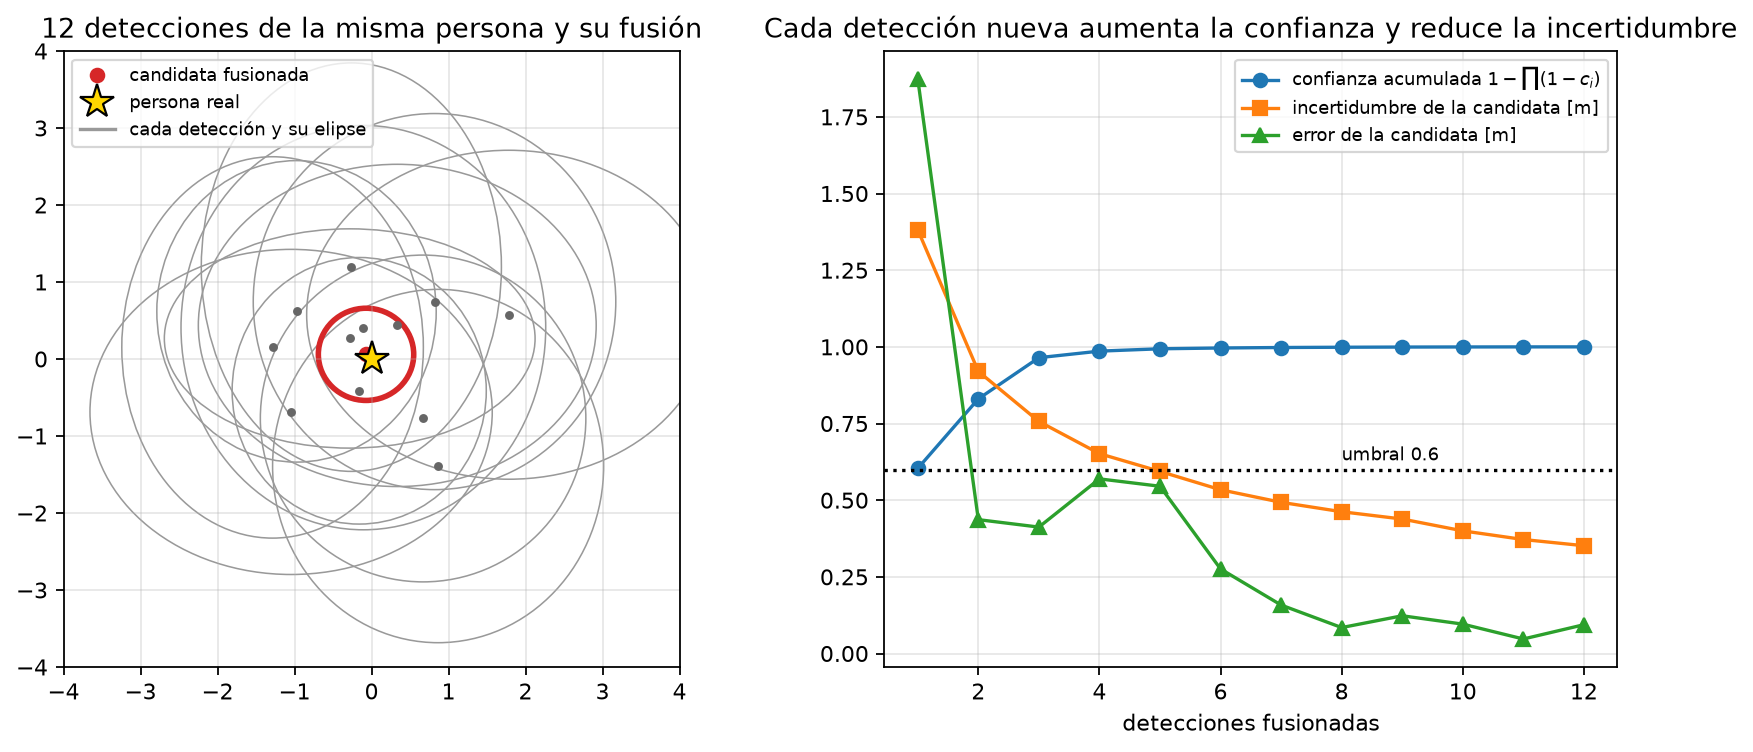
\includegraphics[width=\textwidth]{fusion.png}
\caption{Doce detecciones simuladas de una persona: cada una con su elipse (gris) y la candidata
fusionada (rojo). Con cada detección la confianza sube y la incertidumbre baja.}
\end{figure}

La misión considera \textbf{detectada} a una candidata con confianza acumulada $\ge$ 0.6, y una persona
\textbf{localizada} si alguna detectada queda a menos de 5~m (asignación uno a uno). Las detectadas que
no corresponden a nadie son \textbf{falsas alarmas}.

\begin{leccion}
La confianza acumulada sube muy rápido: dos detecciones de 0.5 ya dan 0.75. Por eso una sombra vista
dos veces ya cuenta como candidata confirmada. En las pruebas, exigir además al menos 10 detecciones
fusionadas bajó las falsas alarmas de 28--31 a 4--5 por vuelo sin perder personas; los avisos GPS usan
ese criterio. Las falsas alarmas que quedan son persistentes: grupos de robles que el detector confunde
una y otra vez.
\end{leccion}

\begin{leccion}
En las vueltas de la ruta el dron se inclina; la cámara, que mira hacia abajo, alcanzaba a ver cerca del
horizonte, y un rayo casi horizontal cortaba el suelo a cientos de metros: salían candidatas a 250~m,
fuera del bosque. El localizador ahora descarta rayos a más de 60° de la vertical (con el dron nivelado
las esquinas de la imagen quedan a $\approx$57°, así que en vuelo normal no se pierde nada).
\end{leccion}

\begin{leccion}
PX4 marca sus mensajes con el reloj de la computadora y la cámara con el de Gazebo. Emparejar cada
imagen con la pose del dron en ese instante exige conocer el desfase; el localizador lo estima con el
mínimo de (llegada $-$ marca) en tiempo simulado.
\end{leccion}


\part{El control: de la cascada a la red neuronal}
\chapter{Control automático desde cero}
\label{cap:control-basico}

\begin{enpocas}
Qué es controlar, la diferencia entre lazo abierto y lazo cerrado, el error, los controladores P, PD
y PID, cómo se lee una respuesta y por qué un dron necesita control en cascada.
\end{enpocas}

\section{¿Qué es controlar?}

Controlar es conseguir que algo se comporte como queremos aunque haya perturbaciones. Queremos que el
dron esté a 30~m de altura; el viento lo empuja hacia abajo; el controlador acelera los motores para
compensar. Al ``algo'' que se controla se le llama \textbf{planta} (aquí, el dron); a lo que queremos,
\textbf{referencia} o \textbf{consigna}; a lo que nos estorba, \textbf{perturbación}.

\section{Lazo abierto y lazo cerrado}

\begin{figure}[H]
\centering
\begin{tikzpicture}[blq/.style={draw,rounded corners,fill=#1,minimum width=2.4cm,minimum height=0.9cm,align=center,font=\small},blq/.default=white,
  fl/.style={-{Stealth[length=2.2mm]},thick}, sum/.style={draw,circle,inner sep=1.5pt}]
  \node at (-1.4,0.9) {\textbf{Lazo abierto}};
  \node (r1) at (-1.2,0) {referencia};
  \node[blq=blue!10] (c1) at (2,0) {controlador};
  \node[blq=orange!15] (p1) at (5.5,0) {planta\\(dron)};
  \node (y1) at (8.6,0) {salida};
  \draw[fl] (r1) -- (c1); \draw[fl] (c1) -- node[above,font=\scriptsize]{acción} (p1); \draw[fl] (p1) -- (y1);
  \node (d1) at (5.5,1.3) {perturbación}; \draw[fl] (d1) -- (p1);

  \node at (-1.4,-1.7) {\textbf{Lazo cerrado}};
  \node (r2) at (-1.2,-2.6) {referencia};
  \node[sum] (s) at (0.5,-2.6) {$-$};
  \node[blq=blue!10] (c2) at (2.6,-2.6) {controlador};
  \node[blq=orange!15] (p2) at (5.9,-2.6) {planta\\(dron)};
  \node (y2) at (9,-2.6) {salida};
  \node[blq=green!12] (sen) at (5.9,-4.1) {sensor};
  \draw[fl] (r2) -- (s); \draw[fl] (s) -- node[above,font=\scriptsize]{error} (c2); \draw[fl] (c2) -- node[above,font=\scriptsize]{acción} (p2);
  \draw[fl] (p2) -- (y2); \draw[fl] (8.1,-2.6) |- (sen); \draw[fl] (sen) -| (s);
  \node (d2) at (5.9,-1.3) {perturbación}; \draw[fl] (d2) -- (p2);
\end{tikzpicture}
\caption{En lazo abierto se actúa ``a ciegas''. En lazo cerrado se mide el resultado, se compara con
lo que se quiere y se corrige: eso es la \emph{retroalimentación}.}
\end{figure}

\begin{ejemplo}
Una tostadora es lazo abierto: tuesta un tiempo fijo, aunque el pan se queme. Ajustar la temperatura
de la regadera es lazo cerrado: sientes el agua (sensor), la comparas con la que quieres (error) y
mueves la llave (acción). Si alguien abre otra llave en la casa (perturbación), lo notas y corriges.
\end{ejemplo}

Un dron sin lazo cerrado no se puede volar: cualquier ráfaga o diferencia entre motores lo voltea
en un segundo. El \textbf{error} es la diferencia entre lo que queremos y lo que hay,
$e = \text{referencia} - \text{medición}$, y todo controlador hace algo con él.

\section{El controlador proporcional (P)}

La idea más simple: actuar en proporción al error. Si estoy 2~m abajo, empujo el doble que si estoy
1~m abajo:
\begin{equation}
u = K_p\, e .
\end{equation}
$K_p$ es la \textbf{ganancia proporcional}. El problema con un dron: el control P actúa sobre la
\emph{aceleración}, y un objeto que se acelera hacia el objetivo llega con velocidad, se pasa,
regresa, se vuelve a pasar... oscila para siempre (curva gris de la figura~\ref{fig:pid}).

\section{El término derivativo (D): frenar a tiempo}

Hay que frenar antes de llegar. El término derivativo actúa sobre la \emph{velocidad} del error: si
me acerco rápido, freno.
\begin{equation}
u = K_p\, e + K_d\, \dot e .
\end{equation}
Es como un amortiguador. Con poco $K_d$ oscila; con mucho, llega muy lento; hay un punto intermedio
(figura~\ref{fig:pid}, derecha).

\section{El término integral (I): no rendirse}

Si un viento constante empuja hacia abajo, el PD llega a un equilibrio un poco por debajo del
objetivo: con ese pequeño error ya compensa el viento. El término integral \emph{acumula} el error en
el tiempo: mientras haya error, sigue creciendo hasta eliminarlo.
\begin{equation}
u = K_p\, e + K_d\, \dot e + K_i\!\int e\,dt .
\end{equation}

\begin{figure}[H]
\centering
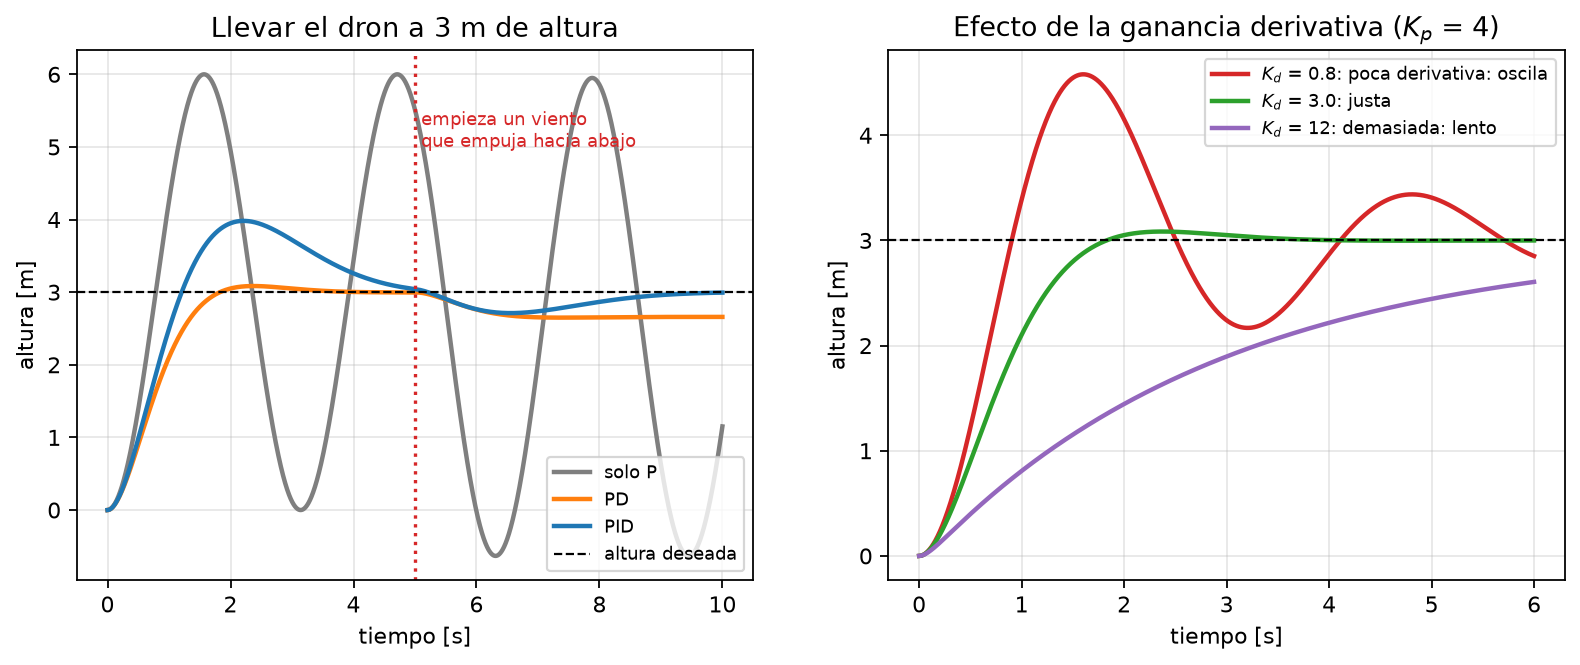
\includegraphics[width=\textwidth]{c_pid.png}
\caption{Simulación de la altura de una masa de 2.2~kg (como un dron mediano). Izquierda: solo P oscila; PD
llega pero el viento (desde $t=5$~s) le deja un error; PID lo corrige. Derecha: efecto de $K_d$.}
\label{fig:pid}
\end{figure}

\begin{recuerda}
\textbf{P} empuja hacia el objetivo, \textbf{D} frena para no pasarse, \textbf{I} corrige lo que
queda. El PID es, de lejos, el controlador más usado en el mundo, incluidos PX4 y ArduPilot.
\end{recuerda}

\section{Cómo se lee una respuesta}

Para comparar controladores se les pide un cambio brusco de referencia (un \textbf{escalón}) y se
mide:

\begin{figure}[H]
\centering
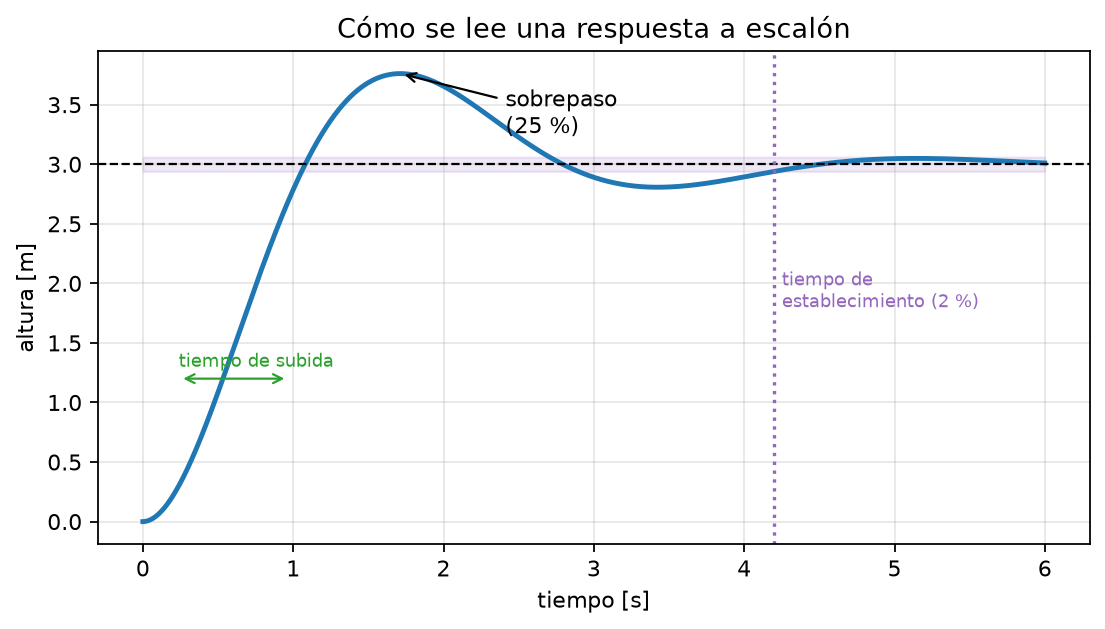
\includegraphics[width=0.8\textwidth]{c_respuesta.png}
\caption{Medidas típicas de una respuesta a escalón.}
\end{figure}

\begin{description}
  \item[Sobrepaso:] cuánto se pasa del objetivo.
  \item[Tiempo de subida:] cuánto tarda en ir del 10~\% al 90~\% del cambio.
  \item[Tiempo de establecimiento:] a partir de cuándo se queda cerca del objetivo (por ejemplo, a
        menos del 2~\%).
  \item[Error en estado estacionario:] lo que queda de error cuando todo se calma.
\end{description}
En este proyecto se usa el \textbf{RMSE de seguimiento}: la raíz del promedio de las distancias al
cuadrado entre el dron y la ruta durante el barrido. Un solo número que resume qué tan bien sigue el dron
su camino.

\section{Control en cascada: así se controla un dron}

El dron no puede ``moverse a la derecha'' directamente: tiene que inclinarse. Por eso hay dos lazos,
uno dentro del otro:

\begin{figure}[H]
\centering
\begin{tikzpicture}[blq/.style={draw,rounded corners,fill=#1,minimum width=2.6cm,minimum height=1cm,align=center,font=\small},blq/.default=white,
  fl/.style={-{Stealth[length=2.2mm]},thick}]
  \node (ref) at (-0.6,0) {\small posición deseada};
  \node[blq=blue!10] (pos) at (2.6,0) {lazos de posición\\y velocidad (lentos)};
  \node[blq=red!10] (act) at (6.4,0) {lazos de actitud\\y de giro (rápidos)};
  \node[blq=black!5] (mix) at (10,0) {mezclador};
  \node[blq=orange!15] (dron) at (10,-2.2) {dron};
  \draw[fl] (ref) -- (pos);
  \draw[fl] (pos) -- node[above,font=\scriptsize,align=center]{empuje e\\inclinación} (act);
  \draw[fl] (act) -- node[above,font=\scriptsize]{pares} (mix);
  \draw[fl] (mix) -- node[right,font=\scriptsize]{4 velocidades} (dron);
  \draw[fl] (dron.west) -- ++(-3,0) -| node[pos=0.75,right,font=\scriptsize]{orientación} (act.south);
  \draw[fl] (dron.west) -- ++(-6.8,0) -| node[pos=0.75,right,font=\scriptsize]{posición} (pos.south);
\end{tikzpicture}
\caption{Control en cascada del cuadrirrotor.}
\label{fig:cascada}
\end{figure}

\begin{enumerate}
  \item El \textbf{lazo de posición} compara dónde está el dron con dónde debe estar y calcula qué
        fuerza total necesita: cuánto empuje y hacia dónde apuntarlo.
  \item Apuntar el empuje significa inclinar el dron: el \textbf{lazo de actitud} calcula los pares
        para alcanzar esa inclinación. Es mucho más rápido que el de posición.
  \item El \textbf{mezclador} convierte empuje y pares en la velocidad de cada motor.
\end{enumerate}
PX4 tiene cuatro lazos en cascada (posición $\rightarrow$ velocidad $\rightarrow$ actitud
$\rightarrow$ velocidad angular), cada uno un P o un PID, que corren a cientos de hertz; ArduPilot hace lo
mismo con otros nombres. Ese es el \textbf{controlador en cascada} del proyecto. La alternativa es
reemplazar toda la cascada por una sola red neuronal que, a partir del estado del dron y del error de
posición, calcula directamente los cuatro motores: el tema del próximo capítulo.

\begin{ejercicio}
Compara la cascada con la red neuronal en la misma misión, sin interfaz:
\begin{lstlisting}[style=bash]
ros2 launch mision simulacion.launch.py gui:=false controlador:=cascada salida:=$HOME/cascada.json
ros2 launch mision simulacion.launch.py gui:=false controlador:=red salida:=$HOME/red.json
\end{lstlisting}
En cada JSON, \cod{rmse_seguimiento} es el error de seguimiento de la ruta y \cod{duracion_s} lo que tardó.
\end{ejercicio}

\chapter{Una red neuronal que vuela el dron}
\label{cap:control-neuronal}

\begin{enpocas}
Qué significa que una red neuronal controle los motores, cómo aprende imitando a un experto
(clonación y DAgger), qué es el aprendizaje por refuerzo (PPO), cómo se mete la red en PX4, qué
problemas tuvo la primera versión y cómo se corrigieron.
\end{enpocas}

\section{La idea}

La cascada de PX4 son cuatro controladores encadenados, con decenas de ganancias ajustadas a mano. La
alternativa es \textbf{una sola red neuronal} que reciba el estado del dron y el error de posición y
calcule directamente los cuatro motores. PX4~1.17 trae un módulo para eso, \cod{mc_nn_control}
(\emph{Neural Control}), con una interfaz fija:

\begin{figure}[H]
\centering
\begin{tikzpicture}[
  n/.style={circle,draw,fill=#1,minimum size=0.42cm,inner sep=0},n/.default=blue!12,
  et/.style={font=\scriptsize,align=right,anchor=east}]
  \foreach \i/\t in {1/{error de posición (3)},4/{fila 1 de $R$ (3)},7/{fila 2 de $R$ (3)},10/{velocidad (3)},13/{velocidad angular (3)}}
    \node[et] at (-0.4,-\i*0.32-0.3) {\t};
  \foreach \i in {1,...,15} \node[n] (a\i) at (0,-\i*0.32) {};
  \foreach \i in {1,...,12} \node[n=orange!20] (b\i) at (2.4,-\i*0.42) {};
  \node at (2.4,-5.4) {\scriptsize 64};
  \foreach \i in {1,...,8} \node[n=orange!30] (c\i) at (4.4,-\i*0.55-0.3) {};
  \node at (4.4,-5.4) {\scriptsize 32};
  \foreach \i in {1,...,4} \node[n=green!20] (d\i) at (6.4,-\i*0.8-0.4) {};
  \foreach \i in {1,...,15} \foreach \j in {1,...,12} \draw[black!12] (a\i) -- (b\j);
  \foreach \i in {1,...,12} \foreach \j in {1,...,8} \draw[black!15] (b\i) -- (c\j);
  \foreach \i in {1,...,8} \foreach \j in {1,...,4} \draw[black!20] (c\i) -- (d\j);
  \foreach \i in {1,...,4} \node[font=\scriptsize,anchor=west] at (6.7,-\i*0.8-0.4) {motor \i: $a_\i\in[-1,1]$};
  \node[font=\small] at (0,0.4) {15 entradas}; \node[font=\small] at (6.4,0.4) {4 salidas};
\end{tikzpicture}
\caption{La red 15-64-32-4 con ReLU: 3\,236 pesos. Entradas en convención ENU-FLU; cada salida se
convierte en la velocidad del motor $\omega_i = \omega_{max}\sqrt{(a_i+1)/2}$.}
\end{figure}

\begin{recuerda}
La red no tiene memoria: en cada instante solo ve el estado actual y el error de posición. No puede
``acumular'' el error como el término integral de un PID. Eso tendrá consecuencias.
\end{recuerda}

\section{Aprender imitando: clonación de comportamiento y DAgger}

¿Cómo se entrena? Lo más directo es \textbf{imitar a un experto}: se vuela con un controlador que ya
funciona (una cascada PD, el ``maestro''), se registran miles de pares (estado, acciones del maestro) y
se entrena la red para que, ante cada estado, dé las mismas acciones. Eso es \textbf{clonación de
comportamiento}, un problema de regresión como cualquier otro.

\begin{ejemplo}
Aprender a manejar viendo a un instructor desde el asiento del copiloto. El problema: el instructor
nunca se sale del carril, así que tú nunca ves cómo se regresa al carril. El día que te desvíes un poco,
no sabrás qué hacer.
\end{ejemplo}

\textbf{DAgger} (\emph{Dataset Aggregation}) resuelve eso: después de la primera ronda, vuela \emph{la
red}, se registran los estados \emph{a los que ella llega} (incluidos sus errores) y el maestro dice qué
habría hecho en cada uno. Se agregan esos ejemplos y se reentrena. Tres rondas bastan. Como el
entrenamiento es en un simulador en Python (el modelo del capítulo de física, a 400~Hz), se agrega
además \textbf{aleatorización de dominio}: en cada episodio la masa, las inercias, $k_f$, el retardo de
los motores y el viento cambian un poco, para que la red no dependa de valores exactos.

\begin{lstlisting}[style=bash]
python3 codigo/nn_imitacion.py --masa 2.114 --com 0.00071 0.00071 --adelanto --salida pesos_nn_x500_busqueda.npz
\end{lstlisting}

\begin{figure}[H]
\centering
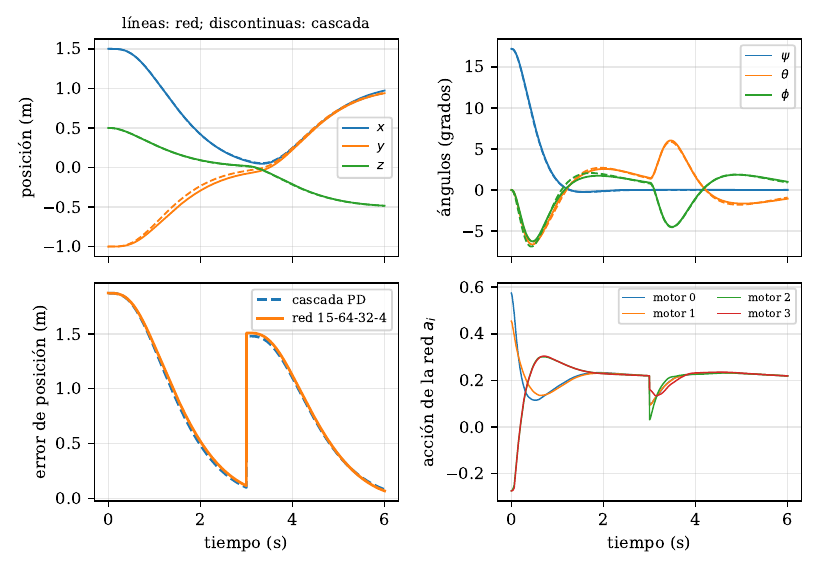
\includegraphics[width=0.85\textwidth]{manual_nn_imitacion_x500_busqueda.png}
\caption{La red (líneas continuas) y el maestro (discontinuas) ante los mismos escalones.}
\end{figure}

\section{Aprender por refuerzo: PPO}

Imitar tiene un techo: la red será, a lo más, tan buena como el maestro. El \textbf{aprendizaje por
refuerzo} quita al maestro: la red prueba acciones, recibe una \textbf{recompensa} (alta si está cerca
del objetivo, baja si se aleja o se estrella) y ajusta sus pesos para aumentar la recompensa acumulada.
\textbf{PPO} (\emph{Proximal Policy Optimization}) es el algoritmo más usado: cambia la política a pasos
pequeños para no destruir lo aprendido. Lleva dos redes: el \emph{actor} (la que vuela) y el
\emph{crítico} (que estima qué tan bueno es cada estado).

La idea del proyecto es partir de la red de imitación y refinarla con PPO
(\cod{codigo/ppo_refinamiento.py}).

\section{De Python a PX4}

\begin{enumerate}
  \item \cod{codigo/exportar_tflite.py} convierte los pesos a \textbf{TensorFlow Lite} (32 bits),
        comprueba que solo use las operaciones que tiene el módulo (capas totalmente conectadas, ReLU y
        suma) y que dé lo mismo que numpy (diferencia de $\sim10^{-6}$), y genera el arreglo en C
        \cod{control_net.cpp/.hpp} (14\,936 bytes).
  \item \cod{scripts/instalar_px4.sh} lo copia a \cod{mc_nn_control} y recompila \cod{px4_sitl_neural}.
  \item La misión cambia al modo \emph{Neural Control} al llegar a la altura de trabajo y regresa a
        offboard antes de aterrizar.
\end{enumerate}
Con ArduPilot, que no tiene un módulo equivalente, la misma red corre en el nodo \cod{controlador_red}
y el plugin \cod{SelectorMotores} deja pasar sus comandos en lugar de los de ArduPilot
(capítulo~\ref{cap:pilotos}).

\begin{leccion}
El diseño original tenía dos detalles que impedían que la red volara: el parámetro
\cod{MC_NN_THRST_COEF} de PX4 trabaja en revoluciones por segundo, no por minuto, y faltaban
\cod{MC_NN_MIN_RPM} y \cod{THR_MDL_FAC}. Con ellos mal, la misma salida de la red producía otro empuje.
Los valores correctos están en el \emph{airframe} \cod{px4/4099_gz_x500_busqueda} y una prueba los
verifica recorriendo toda la cadena de PX4 (red $\rightarrow$ mezclador $\rightarrow$ ESC).
\end{leccion}

\section{Tres problemas de la primera versión y su solución}

\subsection{Un sesgo de 20 cm}

En la primera prueba en SITL quedaba un error permanente en altura de $-0.27$~m: la red se había
entrenado con $m = 2.0$~kg y el x500 completo pesa 2.114~kg. Sin integral, $\Delta z = \Delta m\,g/(m\,k_p)$.
Con la masa correcta el error en altura desapareció, pero quedó un sesgo horizontal de $\approx$0.2~m: la
cámara corre 0.7~mm el centro de masa y la red, que nunca vio ese desequilibrio, se quedaba inclinada
$\approx$1°. La solución fue usar la geometría real en el simulador de entrenamiento (\cod{--com}): el
maestro compensa con los motores y la red aprende a hacerlo.

\subsection{La red iba a la mitad de velocidad}

Una ley PD sin prealimentación, siguiendo una referencia que se mueve a velocidad $v$, se queda atrás
$\frac{k_d}{k_p}v$: con las ganancias del maestro, 4.8~m a 3~m/s. La misión no deja que la consigna se
adelante más de 3~m, así que la red avanzaba a $\approx$1.6~m/s y la misión duraba casi el doble.

La solución clásica de control: mandar una \textbf{consigna adelantada}
\begin{equation}
p_{cons} = p_{ref} + \frac{k_d}{k_p}\,v_{ref}
\quad\Rightarrow\quad
k_p(p_{cons} - p) - k_d v = k_p(p_{ref} - p) + k_d(v_{ref} - v),
\end{equation}
que convierte a la PD en una PD con prealimentación de velocidad, sin cambiar la interfaz de la red.
Pero la red tiene que haber visto esos errores de varios metros: se reentrenó con \cod{--adelanto}
(la mitad de los episodios con referencias que avanzan hasta 4~m/s).

\begin{figure}[H]
\centering
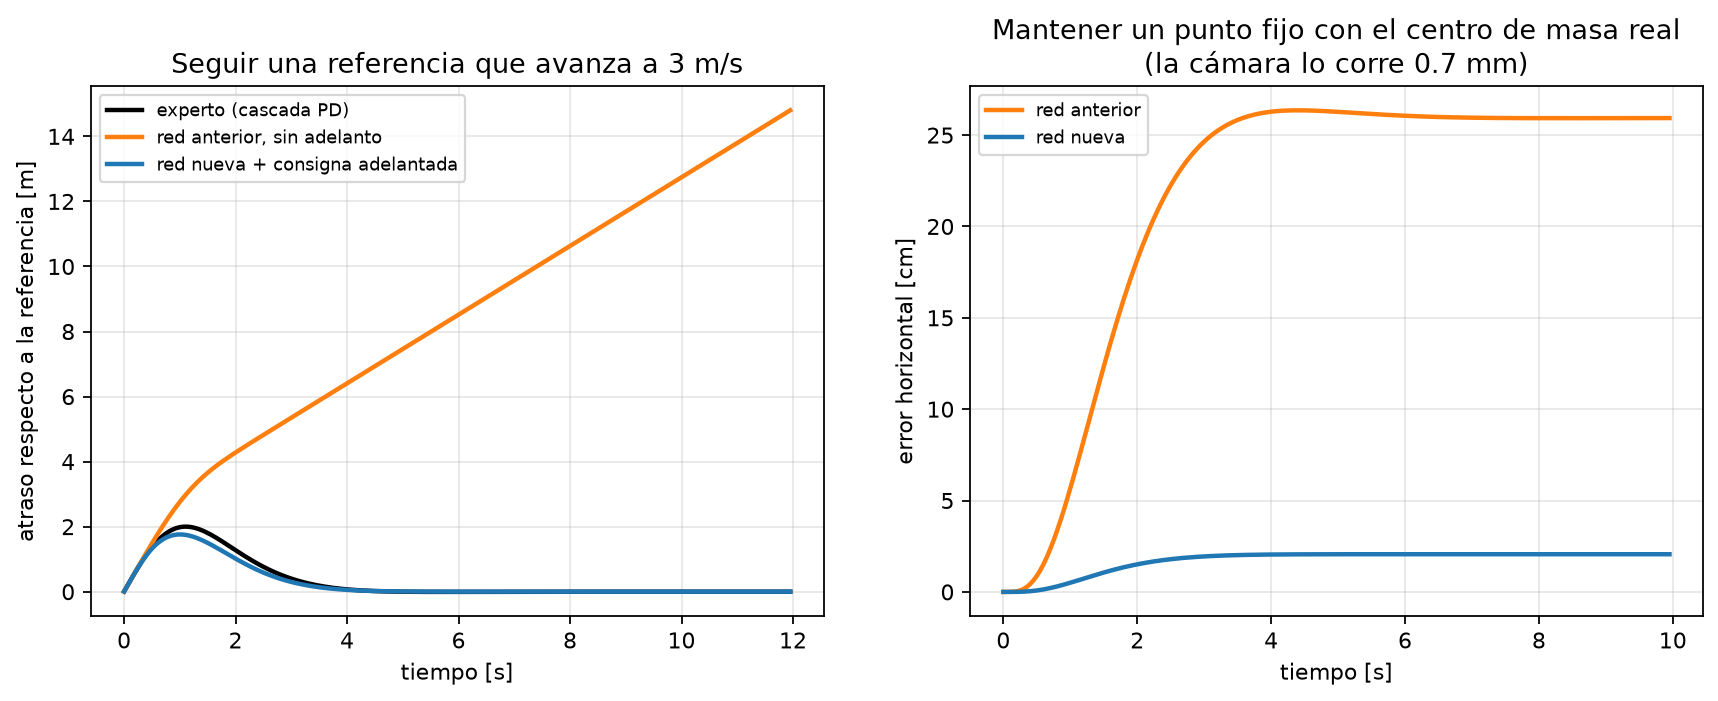
\includegraphics[width=\textwidth]{red_comparacion.png}
\caption{Izquierda: siguiendo una referencia a 3~m/s, la red anterior se atrasa sin parar; la nueva, con
la consigna adelantada, sigue igual que el maestro. Derecha: con el centro de masa real, la red anterior
se queda a 26~cm del punto; la nueva, a 2~cm.}
\end{figure}

\subsection{PPO divergía}

En la primera versión, PPO estaba a la par de la imitación hasta la iteración $\sim$100 y luego se
deterioraba hasta estrellarse en 4 de 40 pruebas. La causa principal estaba en la recompensa original:
cada paso valía $-(|e|^2 + \dots) + 1$, negativo con más de $\sim$1~m de error (hasta $-25$ a 5~m),
mientras que estrellarse costaba solo $-10$ una vez. ¡Terminar pronto ``convenía''! Además los cortes de
episodio por tiempo se trataban como si el dron hubiera fallado, y el crítico, que empieza al azar,
desordenaba la política de imitación en las primeras iteraciones.

La versión mejorada (\cod{--mejorado}) usa una recompensa acotada y positiva mientras el dron vuele,
penaliza estrellarse con $-100$, trata bien los cortes por tiempo, calienta el crítico 15 iteraciones
antes de tocar la política, frena los cambios demasiado grandes (KL) y guarda solo la mejor política.

\begin{figure}[H]
\centering
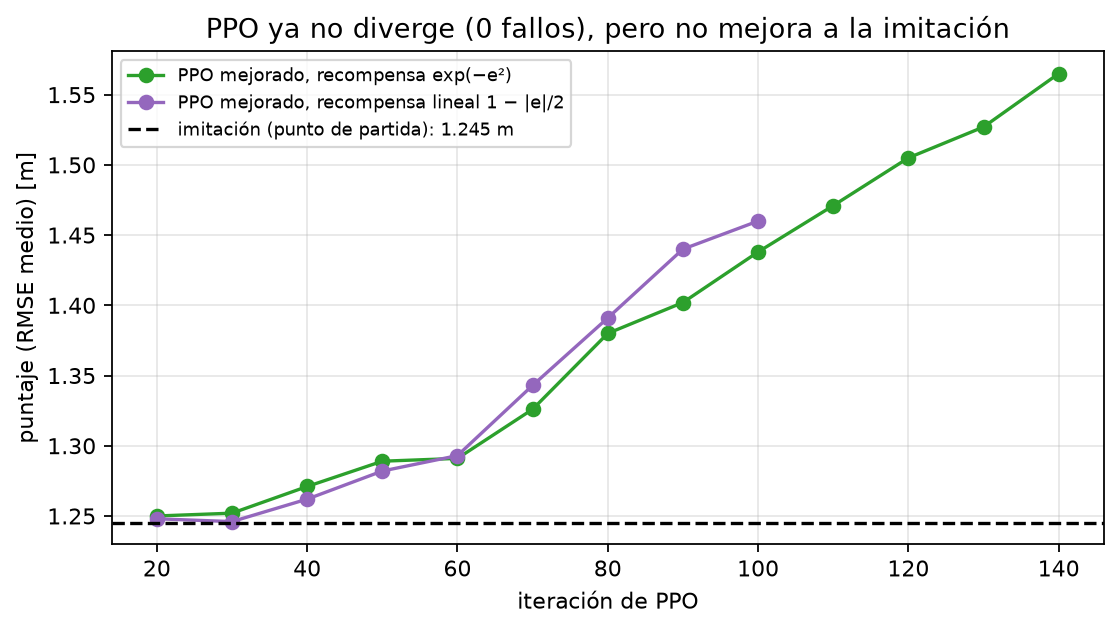
\includegraphics[width=0.8\textwidth]{ppo_curvas.png}
\caption{Con las correcciones PPO ya no diverge (ningún fallo), pero con ninguna de las dos recompensas
probadas mejora a la imitación: se usa la red de imitación.}
\end{figure}

\begin{nota}
Un resultado negativo también es un resultado. Que PPO no mejore aquí es razonable: la red no tiene
memoria y el maestro ya es una buena PD; buena parte del error que queda viene del viento y la masa
aleatorios, que ninguna ley sin integral puede eliminar. Una dirección para mejorarla sería darle a la
red una entrada con el error acumulado, lo que exige modificar el módulo de PX4.
\end{nota}

\section{Resultado en la misión}

\begin{table}[H]
\centering\small
\begin{tabular}{llcccc}
\toprule
\textbf{Piloto} & \textbf{Controlador} & \textbf{Localizadas} & \textbf{Error medio} & \textbf{RMSE ruta} & \textbf{Duración} \\ \midrule
PX4 & cascada & 3/3 & 0.61 m & 0.07 m & 238 s \\
PX4 & red anterior & 3/3 & 0.71 m & 0.11 m & 427 s \\
PX4 & red nueva & 3/3 & 0.52 m & 0.23 m & \textbf{211 s} \\
ArduPilot & red anterior & 3/3 & 0.46 m & 0.12 m & 451 s \\
ArduPilot & red nueva & 3/3 & 0.47 m & 0.19 m & \textbf{240 s} \\
\bottomrule
\end{tabular}
\caption{La misma misión (bosque medio, sol alto, sin viento, 3 personas). Con la red nueva la misión
dura la mitad, igual o menos que con la cascada; sigue la ruta algo peor en las esquinas, donde la
consigna adelantada cambia de dirección de golpe.}
\end{table}


\part{Construir la simulación}
\chapter{Instalación paso a paso}
\label{cap:instalacion}

\begin{enpocas}
Qué hay que instalar y en qué orden: ROS~2 y Gazebo, PX4 con el módulo neuronal, el agente uXRCE-DDS,
el workspace, ArduPilot y los entornos de Python. Todo está en \cod{scripts/instalar_entorno.sh},
pensado para correrse bloque por bloque y sin \cod{sudo} salvo donde se indica.
\end{enpocas}

\section{0. ROS 2 Jazzy y Gazebo Harmonic}

Ubuntu 24.04 con ROS~2 Jazzy y el puente \cod{ros-jazzy-ros-gz} (que trae Gazebo Harmonic), instalados
con el repositorio oficial de ROS~2 (\cod{ros-jazzy-desktop}, \cod{ros-dev-tools},
\cod{ros-jazzy-ros-gz}).

\section{1. PX4 release/1.17}

\begin{lstlisting}[style=bash]
cd ~ && git clone --recursive -b release/1.17 https://github.com/PX4/PX4-Autopilot.git
python3 -m venv --system-site-packages ~/.venvs/px4
~/.venvs/px4/bin/pip install -r ~/PX4-Autopilot/Tools/setup/requirements.txt ninja
\end{lstlisting}

\begin{aviso}
La etiqueta \cod{v1.17.0} de PX4 no existe (solo \cod{v1.17.0-rc2}): se usa la rama \cod{release/1.17}.
Ubuntu 24.04 no deja instalar con \cod{pip install --user} sobre el Python del sistema (PEP 668): por eso
cada grupo de dependencias va en su propio entorno.
\end{aviso}

\section{2. Agente Micro XRCE-DDS 2.4.3}

\begin{lstlisting}[style=bash]
cd ~ && git clone -b v2.4.3 https://github.com/eProsima/Micro-XRCE-DDS-Agent.git
cd Micro-XRCE-DDS-Agent && mkdir build && cd build
env -i HOME=$HOME PATH=/usr/bin:/bin cmake .. -DCMAKE_INSTALL_PREFIX=$HOME/.local
env -i HOME=$HOME PATH=/usr/bin:/bin make -j"$(nproc)" && make install
\end{lstlisting}
Se compila con un entorno limpio (\cod{env -i}) para que use su propio Fast-DDS y no el de ROS, y se
instala en \cod{~/.local} sin \cod{sudo}.

\section{3. Workspace}

\begin{lstlisting}[style=bash]
git clone https://github.com/jairoroke/<repositorio>.git ~/ros2_ws
cd ~/ros2_ws/src
git clone -b release/1.17 https://github.com/PX4/px4_msgs.git
git clone https://github.com/ArduPilot/ardupilot_gazebo.git       # solo para piloto:=ardupilot
cd ~/ros2_ws && colcon build --symlink-install && source install/setup.bash
\end{lstlisting}

\section{4. Entornos de Python}

\begin{lstlisting}[style=bash]
python3 -m venv ~/venv-mision
~/venv-mision/bin/pip install numpy scipy matplotlib pillow tensorflow-cpu    # exportar la red
\end{lstlisting}
\begin{itemize}
  \item \cod{~/venv-mision}: TensorFlow, para exportar la red a TFLite.
  \item \cod{~/.venvs/yolo}: Ultralytics con PyTorch y CUDA (y \cod{numpy<2}, para leer los mensajes de
        ROS~2). Corre el detector y el refinamiento PPO.
  \item \cod{~/venv-ardupilot}: MAVProxy, pymavlink y \cod{python-xlib} (para acomodar las ventanas).
\end{itemize}

\section{5. Vehículo, red y compilación de PX4}

\begin{lstlisting}[style=bash]
cd ~/ros2_ws/src/mision
python3 scripts/generar_vehiculo.py      # tarot650_busqueda, x500_busqueda y sus variantes para ArduPilot
cd codigo
python3 nn_imitacion.py --vehiculo tarot650 --masa 2.25 --com 0.00067 0.00067 --adelanto \
    --salida pesos_nn_tarot650_busqueda.npz --figura ../imagenes/nn_imitacion_tarot650_busqueda.pdf
~/venv-mision/bin/python exportar_tflite.py --pesos pesos_nn_tarot650_busqueda.npz --salida control_net_tarot650_busqueda
bash ../scripts/instalar_px4.sh ~/ros2_ws/src/mision/codigo/control_net_tarot650_busqueda
\end{lstlisting}
\cod{instalar_px4.sh} copia a \cod{~/PX4-Autopilot} los vehículos \cod{tarot650_busqueda} y
\cod{x500_busqueda}, los \emph{airframes} \cod{4100_gz_tarot650_busqueda} y \cod{4099_gz_x500_busqueda}
(carpeta \cod{px4/}) y la red (guardando una vez la original como \cod{control_net.*.px4}), agrega
\cod{/fmu/out/neural_control} a los tópicos que exporta PX4 y compila \cod{make px4_sitl_neural}.
Repite estos pasos cada vez que cambies la red o el vehículo.

\begin{aviso}
PX4 lleva \textbf{una sola red compilada}: ahora es la del Tarot. Para volar el x500 con
\cod{controlador:=red} en PX4 hay que reinstalar \cod{control_net_x500_busqueda}. Con ArduPilot no
hace falta: \cod{controlador_red} carga los pesos del vehículo que se lanza.
\end{aviso}

\section{6. ArduPilot (opcional)}

ArduCopter 4.7.2 compilado para SITL en \cod{~/ardupilot} (\cod{./waf configure --board sitl \&\& ./waf
copter}) y el plugin \cod{ardupilot_gazebo} en el workspace.

\section{Comprobación}

\begin{lstlisting}[style=bash]
cd ~/ros2_ws/src/mision && python3 -m pytest -q test/          # 8 pruebas
ros2 launch mision simulacion.launch.py gui:=false              # una misión completa, unos 4 min
\end{lstlisting}

\chapter{Dónde está cada cosa}

\begin{lstlisting}
~/ros2_ws/src/
|-- mision/                    paquete principal (Python)
|   |-- mision/                nodos de ROS 2 y bibliotecas
|   |-- codigo/                programas de referencia y la red neuronal
|   |-- launch/simulacion.launch.py
|   |-- scripts/               generadores, dataset, entrenamiento, campaña, instalación
|   |-- models/                x500_busqueda, personas, árboles, suelo
|   |-- px4/                   airframe 4099_gz_x500_busqueda
|   |-- config/                GUI de Gazebo, parámetros de ArduPilot
|   |-- yolo/                  personas_yolo26s.pt (detector)
|   `-- test/                  pruebas (pytest)
|-- mision_gz_plugins/         SelectorMotores (C++), para ArduPilot con la red
|-- px4_msgs/                  mensajes de PX4 (clonado, release/1.17)
`-- ardupilot_gazebo/          plugin de ArduPilot (clonado)
\end{lstlisting}

\section{Nodos y módulos}

\begin{longtable}{>{\raggedright\arraybackslash}p{4.3cm}p{10.8cm}}
\toprule
\textbf{Archivo} & \textbf{Qué hace} \\ \midrule \endhead
\cod{detector_node.py} & YOLO sobre \cod{/camera}; publica \cod{/detecciones} y la imagen anotada. \\
\cod{localizador_node.py} & Rayo--terreno, covarianza, asociación de Mahalanobis y fusión. \\
\cod{mision_node.py} & Barrido offboard, re-observación, Neural Control, avisos GPS, evasión, métricas. \\
\cod{mision_ardupilot.py} & La misma misión con ArduCopter (GUIDED por MAVLink). \\
\cod{controlador_red.py} & La red como controlador de motores con ArduPilot. \\
\cod{geometria.py} & Proyección, localización y covarianza (compartidas con las pruebas). \\
\cod{metricas.py} & Personas localizadas, falsas alarmas, error, distancia a la ruta. \\
\cod{evasion.py}, \cod{geo.py} & Evasión con el LiDAR; conversión ENU $\rightarrow$ GPS. \\
\cod{mavproxy_trayectoria.py}, \cod{ventanas_sitl.py} & Mapa de MAVProxy con ruta y personas; acomodo de ventanas. \\
\cod{modo_neural.py}, \cod{prueba_neural.py} & Activar Neural Control a mano; escalones de prueba. \\
\bottomrule
\end{longtable}

\section{Programas de referencia (\texorpdfstring{\texttt{codigo/}}{codigo/})}

\begin{longtable}{>{\raggedright\arraybackslash}p{4.3cm}p{10.8cm}}
\toprule
\cod{sim_modelo.py} & Modelo del x500 con el control base. \\
\cod{sim_localizacion.py} & Localización, covarianza y Monte Carlo. \\
\cod{nn_imitacion.py} & Red 15-64-32-4 por clonación + DAgger (\cod{--masa}, \cod{--com}, \cod{--adelanto}). \\
\cod{ppo_refinamiento.py} & Refinamiento por PPO (\cod{--mejorado}, \cod{--forma}). \\
\cod{exportar_tflite.py} & TFLite y \cod{control_net.cpp/.hpp}. \\
\bottomrule
\end{longtable}
Sin las opciones nuevas, estos programas reproducen exactamente las cifras de referencia.

\section{Scripts}

\begin{longtable}{>{\raggedright\arraybackslash}p{4.3cm}p{10.8cm}}
\toprule
\cod{generar_mundo.py} & Bosque por oclusión, iluminación, viento y semilla, con el JSON de las personas verdaderas. \\
\cod{generar_vehiculo.py} & El x500 con cámara bajo los patines, viento y LiDAR. \\
\cod{capturar_dataset.py}, \cod{entrenar_detector.py} & Dataset con cajas visibles y entrenamiento por estrato. \\
\cod{correr_experimentos.py}, \cod{analisis_wilcoxon.py} & Campaña factorial y pruebas estadísticas. \\
\cod{instalar_entorno.sh}, \cod{instalar_px4.sh} & Instalación. \\
\bottomrule
\end{longtable}

\chapter{El Tarot 650 en Gazebo}
\label{cap:tarot650}

\begin{enpocas}
De dónde sale el vehículo de la simulación, qué se le agregó para que lo vuele PX4, cuáles de sus datos
son supuestos y cómo se cambian por los del dron real, cómo es su variante para ArduPilot y cómo volar
todavía con el x500 de las primeras corridas.
\end{enpocas}

\section{El tarot650\_busqueda}

El vehículo es el \textbf{Tarot Ironman 650}. Su modelo de Gazebo, \cod{tarot650_busqueda}, lo arma
\cod{scripts/generar_vehiculo.py} con dos fuentes:
\begin{itemize}
  \item \textbf{Del Tarot:} las mallas de su CAD (placas, brazos, motores, tren de aterrizaje y hélices,
        carpeta \cod{models/tarot650_busqueda/meshes}), la masa, las inercias, la posición de los
        rotores, las hélices y los motores. Todo sale de la tabla \cod{VEHICULOS['tarot650']} de
        \cod{cuadrirotor_sim/scripts/generar_modelo.py}, otro paquete del mismo \emph{workspace}, así
        que los dos proyectos usan el mismo dron.
  \item \textbf{Del x500 de PX4:} los sensores (IMU, barómetro, magnetómetro y GPS, con el ruido de PX4)
        y con los mismos nombres, porque el puente de PX4 con Gazebo los busca así.
\end{itemize}
Además, \cod{generar_vehiculo.py} pone los motores en el orden de PX4 (\cod{rotor_0} adelante-derecha
antihorario, \cod{rotor_1} atrás-izquierda antihorario, \cod{rotor_2} adelante-izquierda horario,
\cod{rotor_3} atrás-derecha horario), que es también el de las salidas 1--4 de ArduPilot en un ``X'', y
le agrega:
\begin{enumerate}
  \item \textbf{La cámara 24~cm debajo del centro}, justo bajo los patines, mirando hacia abajo
        (la \cod{mono_cam} de PX4: $1280\times960$, campo horizontal de 1.74~rad).
  \item \textbf{Viento habilitado} en el cuerpo (\cod{<enable_wind>}), para que el sistema
        \cod{WindEffects} del mundo lo empuje.
  \item \textbf{Un LiDAR 3D} (360°$\times$120 haces, 16 canales de $-35$° a $+15$°, 30~m, 10~Hz,
        \cod{/dron/lidar/points}) para la evasión de obstáculos.
\end{enumerate}

\begin{table}[H]
\centering\small
\begin{tabular}{ll}
\toprule
\textbf{Parámetro} & \textbf{Valor} \\ \midrule
Masa total & 2.25~kg (cuerpo 2.12, rotores $4\times20$~g, cámara 50~g) \\
Inercia del cuerpo & diag(0.0304, 0.0321, 0.0585)~kg\,m$^2$ \\
Inercia con los rotores & diag(0.0341, 0.0361, 0.0660)~kg\,m$^2$ \\
Rotores & $(\pm0.2198, \pm0.212)$~m, 4~cm sobre el centro, hélices de 15'' \\
$k_f$, $k_m$, $\omega_{max}$ & $4.24\times10^{-5}$~N/(rad/s)$^2$, 0.016~m, 680~rad/s \\
Empuje máximo & 19.6~N por motor, $\approx$3.6 veces el peso en total \\
Vuelo estacionario & $\omega_h = 361$~rad/s por motor \\
Constantes de tiempo de los motores & 0.03~s al subir, 0.05~s al bajar \\
Cámara & $1280\times960$, HFOV 1.74~rad, hacia abajo, $t_{BC} = (0, 0, -0.24)$~m \\
Centro de masa & corrido 0.67~mm en $x$ y en $y$ por la cámara \\
\bottomrule
\end{tabular}
\caption{Parámetros del Tarot 650 de la simulación (\cod{models/tarot650_busqueda/model.sdf} y la tabla
\cod{VEHICULOS} de \cod{codigo/nn_imitacion.py}). Los de masa, inercias, $k_f$ y motores son supuestos.}
\end{table}

El \emph{airframe} de PX4 es \cod{px4/4100_gz_tarot650_busqueda}. Además de la geometría de los rotores
(\cod{CA_ROTOR*}), fija las salidas a los motores de Gazebo entre 100 y 680~rad/s
(\cod{SIM_GZ_EC_MIN}, \cod{SIM_GZ_EC_MAX}), el empuje de vuelo estacionario (\cod{MPC_THR_HOVER} 0.25,
con \cod{THR_MDL_FAC} 0.8) y los parámetros del modo \emph{Neural Control} para la red del Tarot
(\cod{MC_NN_THRST_COEF} 17.0754, \cod{MC_NN_MIN_RPM} 955, \cod{MC_NN_MAX_RPM} 6494; capítulo
\ref{cap:control-neuronal}).

\begin{tecnico}
¿De dónde sale \cod{MPC_THR_HOVER} = 0.25? En vuelo estacionario, $\omega_h = 361$~rad/s. La salida
normalizada del motor es $(361-100)/580 = 0.45$ y, con la curva $0.8x^2 + 0.2x$ que PX4 deshace con
\cod{THR_MDL_FAC} = 0.8, el empuje normalizado es $0.8(0.45)^2 + 0.2(0.45) \approx 0.25$.
\end{tecnico}

\section{Supuestos que hay que reemplazar}

\begin{aviso}
La masa, las inercias, $k_f$ y los retardos de los motores del Tarot de la simulación son
\textbf{supuestos}: no se midieron en un dron real. Las mallas dan la forma, no la física. Antes de
llevar la red neuronal o las ganancias a un Tarot real hay que reemplazarlos por los de ese dron.
\end{aviso}

Los pasos, en orden:
\begin{enumerate}
  \item Mide la masa (con batería, cámara y todo lo que vaya a volar), las inercias, $k_f$ y $k_m$ (en
        un banco de empuje) y la respuesta de los motores.
  \item Ponlos en la tabla \cod{VEHICULOS['tarot650']} de \cod{cuadrirotor_sim/scripts/generar_modelo.py}
        y en la de \cod{codigo/nn_imitacion.py}, y vuelve a generar el vehículo
        (\cod{python3 scripts/generar_vehiculo.py}).
  \item Si cambian la posición de los rotores, $\omega_{max}$ o el empuje de vuelo estacionario, ajusta el
        \emph{airframe} \cod{px4/4100_gz_tarot650_busqueda} y \cod{config/ardupilot/tarot650.parm}.
  \item Reentrena la red (\cod{nn_imitacion.py --vehiculo tarot650 --masa ... --com ...}), expórtala e
        instálala en PX4 (capítulo~\ref{cap:instalacion}).
\end{enumerate}

\section{La variante para ArduPilot}

\cod{tarot650_busqueda_ardupilot} es el mismo vehículo con:
\begin{itemize}
  \item \cod{ArduPilotPlugin}, que intercambia sensores y motores con ArduCopter (salidas de
        1000--2000~µs $\rightarrow$ 0--680~rad/s, mismo orden de motores que PX4);
  \item una IMU para ArduPilot, con ruido y sesgo supuestos (giróscopo 0.004~rad/s, acelerómetro
        0.1~m/s$^2$), y \cod{OdometryPublisher} a 400~Hz (el estado para la red);
  \item \cod{no_time_sync=0}, para que ArduPilot vuele con su EKF3 y no con el estado verdadero del
        simulador (capítulo~\ref{cap:pilotos});
  \item el sistema \cod{SelectorMotores} (paquete \cod{mision_gz_plugins}), que deja pasar los comandos
        de ArduPilot o los de la red, según lo que pida la misión.
\end{itemize}
En esa variante el vehículo va dentro del mundo, que corre a 1~kHz (lo que espera ArduPilot). Sus
parámetros de vuelo están en \cod{config/ardupilot/tarot650.parm}: salidas de 1000--2000~µs con curva
de empuje cuadrática pura (\cod{MOT_THST_EXPO} 1.0), \cod{MOT_THST_HOVER} 0.28 ($(361/680)^2$), lazos
de tasa más suaves que los del Iris (el Tarot tiene motores más lentos) y \cod{AHRS_EKF_TYPE} 3.

\begin{lstlisting}[style=bash]
python3 scripts/generar_vehiculo.py      # escribe models/tarot650_busqueda, models/x500_busqueda y sus variantes _ardupilot
bash scripts/instalar_px4.sh ~/ros2_ws/src/mision/codigo/control_net_tarot650_busqueda    # y los copia a PX4
\end{lstlisting}

\section{El x500 de PX4 sigue disponible}

Las primeras corridas, las del 22 y el 23 de octubre, se hicieron con el \textbf{x500} de PX4, y varias
cifras del libro vienen de ellas. El vehículo sigue en el paquete y se elige con un argumento:
\begin{lstlisting}[style=bash]
ros2 launch mision simulacion.launch.py vehiculo:=x500
\end{lstlisting}
\cod{x500_busqueda} parte del \cod{x500_mono_cam_down} de PX4 con los mismos tres cambios (cámara bajo los
patines, viento y LiDAR); usa el \emph{airframe} \cod{4099_gz_x500_busqueda}, \cod{config/ardupilot/x500.parm}
y la red \cod{pesos_nn_x500_busqueda.npz} / \cod{control_net_x500_busqueda}.

\begin{figure}[H]
\centering
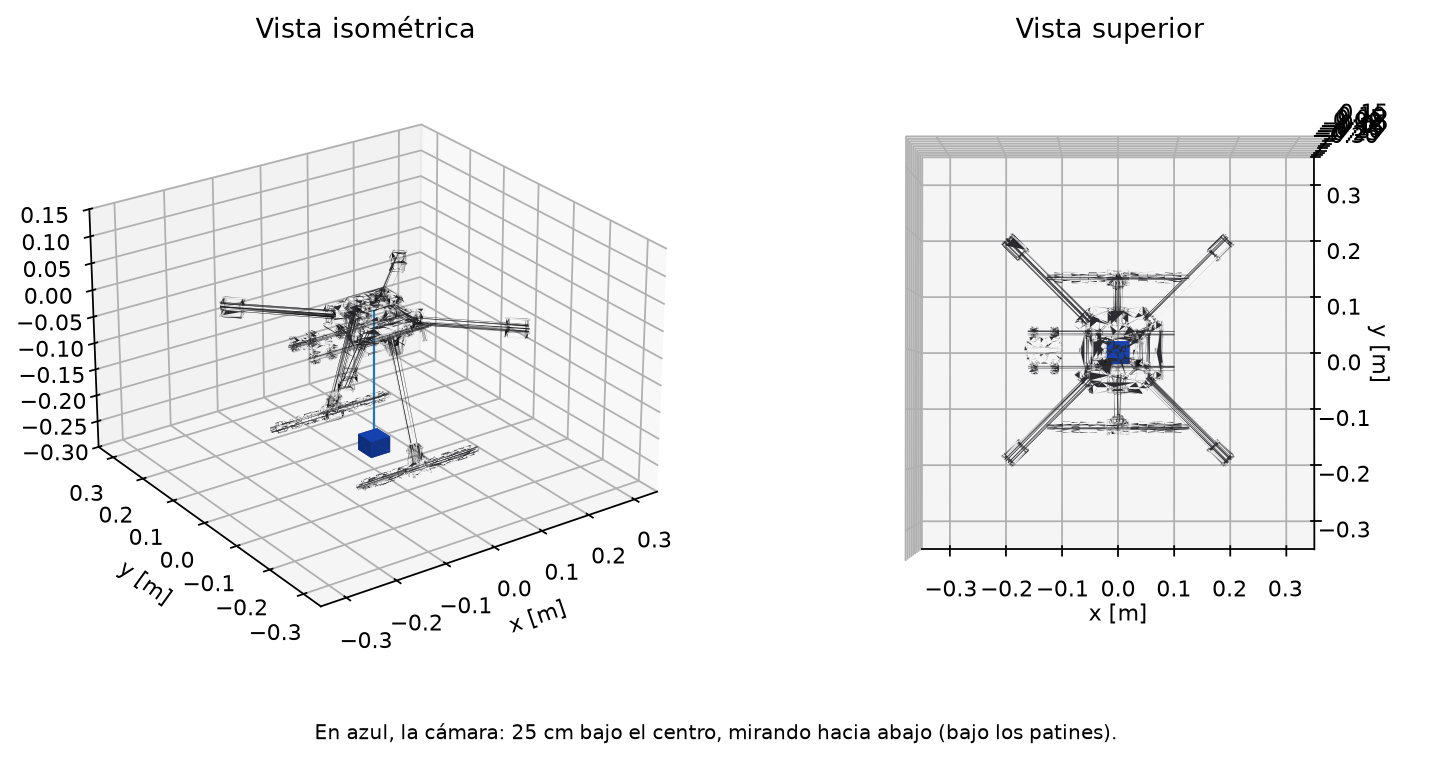
\includegraphics[width=0.85\textwidth]{x500_render.png}
\caption{El x500 de PX4, dibujado a partir de las mallas de su modelo.}
\end{figure}

\begin{table}[H]
\centering\small
\begin{tabular}{ll}
\toprule
\textbf{Parámetro} & \textbf{Valor} \\ \midrule
Masa total & 2.114~kg (cuerpo 2.0, rotores $4\times16$~g, cámara 50~g) \\
Inercia del cuerpo & diag(0.0217, 0.0217, 0.040)~kg\,m$^2$ \\
Rotores & $(\pm0.174, \pm0.174)$~m, hélices de 13'' \\
$k_f$, $k_m$, $\omega_{max}$ & $8.54858\times10^{-6}$~N/(rad/s)$^2$, 0.016~m, 1000~rad/s \\
Constantes de tiempo de los motores & 12.5~ms al subir, 25~ms al bajar \\
Cámara & $1280\times960$, HFOV 1.74~rad, hacia abajo, $t_{BC} = (0, 0, -0.25)$~m \\
Centro de masa & corrido 0.7~mm en $x$ y en $y$ por la cámara \\
\bottomrule
\end{tabular}
\caption{Parámetros del x500 de la simulación.}
\end{table}

\begin{leccion}
En el modelo de PX4 la cámara está 10~cm \emph{arriba} del centro y mira hacia abajo a través del
cuerpo: el armazón, los motores y el tren de aterrizaje tapaban más de la mitad de la imagen. El diseño
original suponía 10~cm \emph{abajo}. En el x500 la cámara se movió 25~cm abajo y en el Tarot va 24~cm
abajo; el localizador usa el valor de cada vehículo ($t_{BC}$, parámetro \cod{z_camara} que le pasa
el \emph{launch}).
\end{leccion}

\begin{aviso}
PX4 lleva una sola red compilada, y ahora es la del Tarot. Para volar el x500 con \cod{controlador:=red}
en PX4 hay que reinstalar la suya:
\cod{bash scripts/instalar_px4.sh ~/ros2_ws/src/mision/codigo/control_net_x500_busqueda}. Con ArduPilot
no hace falta: \cod{controlador_red} carga los pesos del vehículo que se lanza.
\end{aviso}

\section{Las personas}

Cuatro modelos de OpenRobotics (Gazebo Fuel, CC0): de pie, caminando, mujer y sentada (Rescue Randy),
todos estáticos y con la etiqueta~1 del sistema \cod{Label}. La persona acostada es uno de pie girado
90°. Los copia y adapta \cod{scripts/importar_personas.py}.

\begin{figure}[H]
\centering
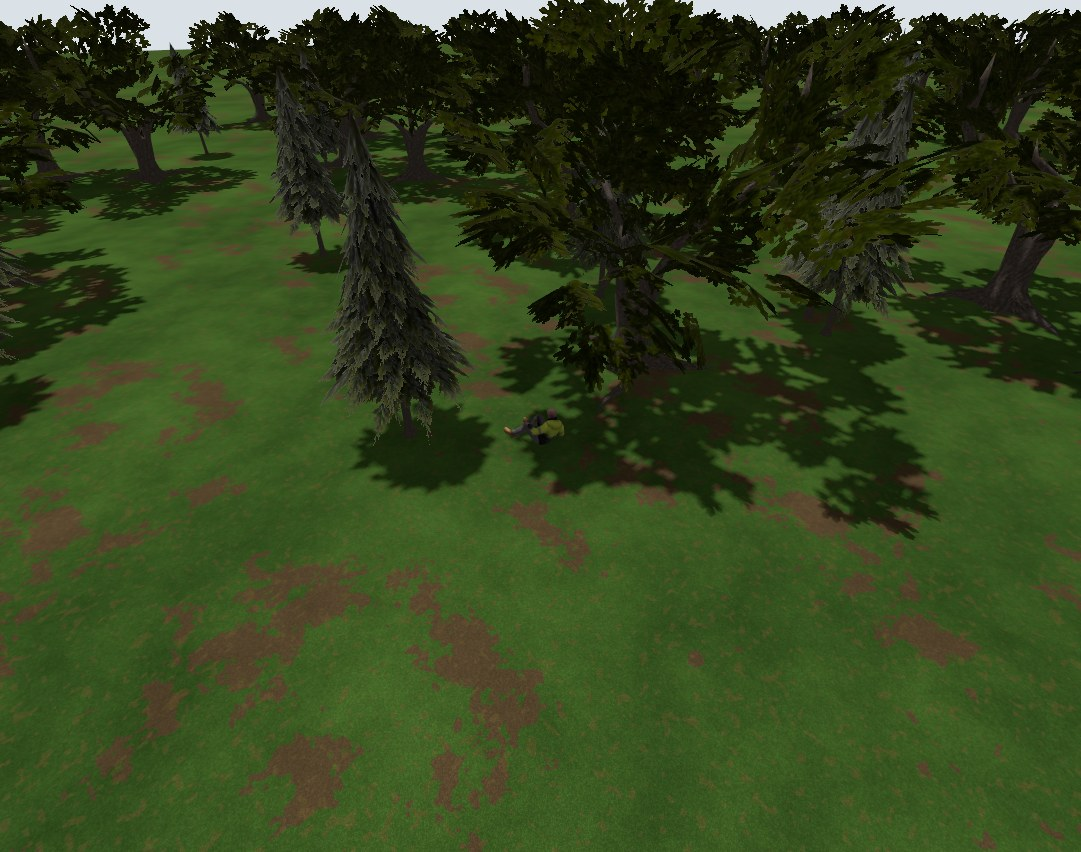
\includegraphics[width=0.6\textwidth]{gz_persona_sentada.jpg}
\caption{Una persona sentada bajo los árboles: desde arriba, una copa puede taparla por completo.}
\end{figure}

\chapter{Un bosque hecho por factores}
\label{cap:bosque}

\begin{enpocas}
Cómo se genera cada bosque a partir de cuatro factores (oclusión, iluminación, viento y semilla), cómo
se mide la cobertura de copas y dónde se colocan las personas.
\end{enpocas}

\section{Por qué un bosque ``por factores''}

Para saber si una estrategia de búsqueda es mejor que otra hay que compararlas en condiciones
controladas: el mismo bosque, las mismas personas, cambiando una cosa a la vez. Por eso cada bosque se
genera a partir de \textbf{factores}:
\begin{description}
  \item[Oclusión] (baja, media, alta): fracción del suelo cubierta por copas, 15, 45 y 75~\%.
  \item[Iluminación] (alta, baja): sol de mediodía o sombras largas de tarde.
  \item[Viento] (no, sí): 4~m/s medios con ráfagas (\cod{WindEffects}).
  \item[Semilla:] un número que fija dónde quedan los árboles y las personas; con la misma semilla
        sale exactamente el mismo bosque.
\end{description}

\begin{lstlisting}[style=bash]
python3 scripts/generar_mundo.py --oclusion media --iluminacion alta --viento no --semilla 1 --salida ~/mundos
\end{lstlisting}

\section{Cobertura de copas}

Los robles miden 10~m de diámetro de copa y los pinos 3.2~m. El generador coloca árboles al azar y, sobre
una rejilla de 0.5~m, mide qué fracción del cuadrado de $120\times120$~m queda bajo alguna copa; se
detiene al llegar a la cobertura pedida. Deja libres 8~m alrededor del despegue.

\begin{figure}[H]
\centering
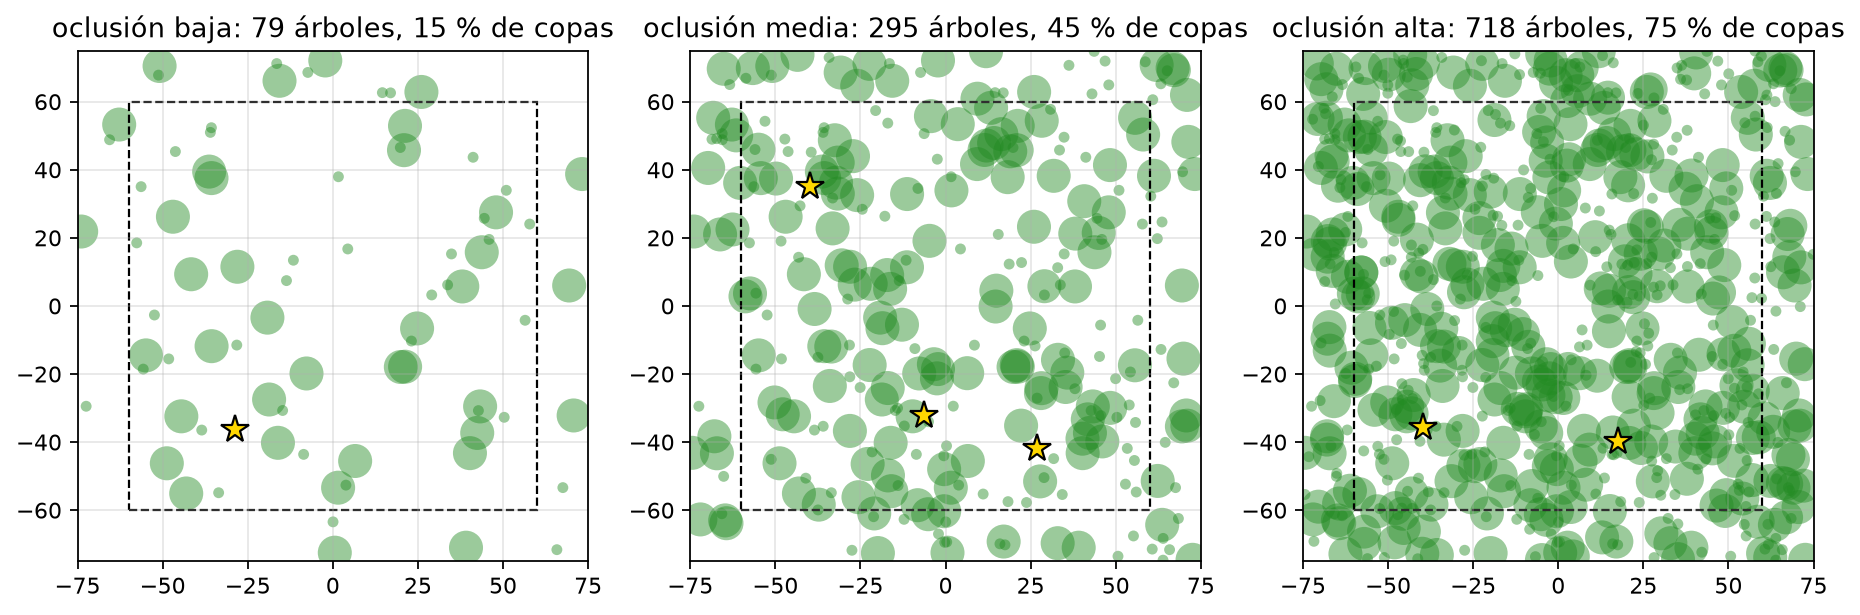
\includegraphics[width=\textwidth]{bosques_oclusion.png}
\caption{Los tres niveles de oclusión con la misma semilla: 79, 295 y 718 árboles. Las estrellas son
las personas.}
\end{figure}

\begin{nota}
Las densidades fijas del diseño original (60, 160 y 280 árboles por hectárea) suponían copas de 6~m; con
los robles de Gazebo Fuel (10~m) daban otra cobertura. Por eso aquí el nivel se define por la cobertura
medida, que es lo que de verdad importa para la cámara, y la densidad resultante se guarda en el JSON.
\end{nota}

\section{Las personas}

De una a tres personas (o las que se pidan con \cod{personas:=}), en posiciones al azar a más de 10~m
del borde, en tres poses: de pie, sentada o acostada. Sus posiciones exactas se guardan en
\cod{personas_<mundo>.json}: la ``verdad'' contra la que se miden los resultados, que la misión nunca
usa para decidir.

\begin{figure}[H]
\centering
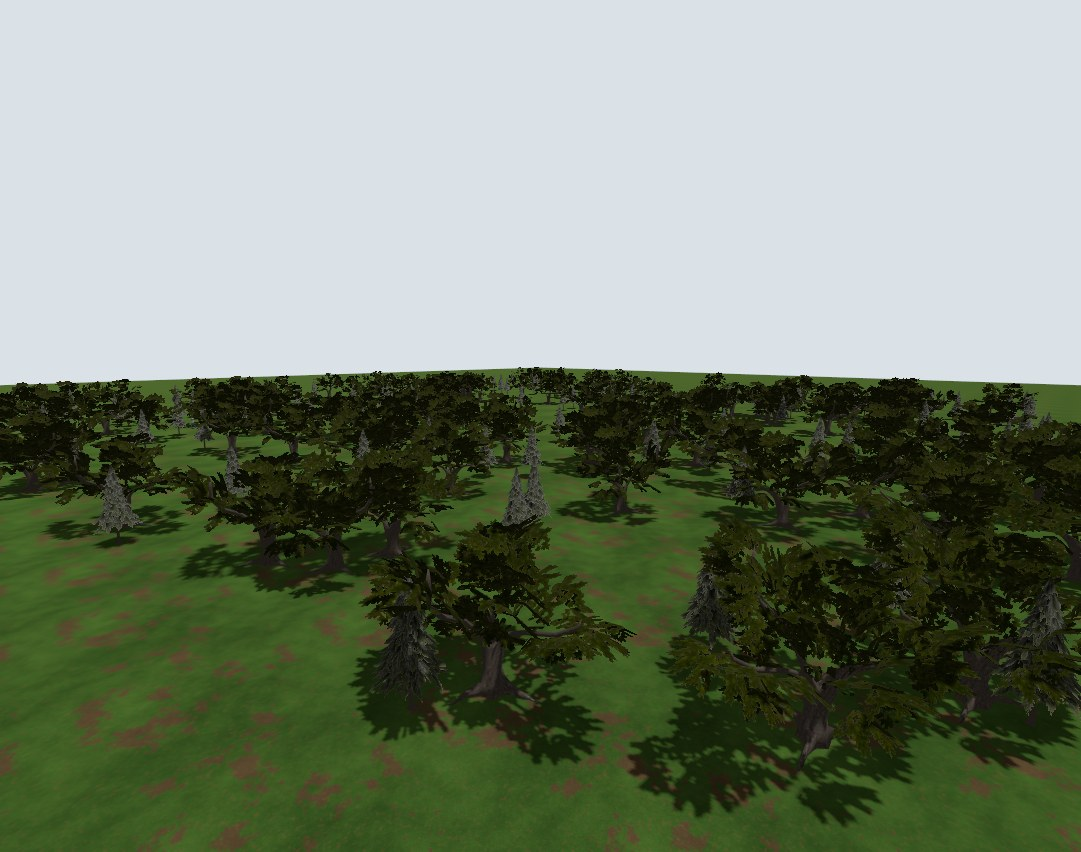
\includegraphics[width=0.8\textwidth]{gz_bosque_bajo.jpg}
\caption{El bosque de oclusión media visto a baja altura.}
\end{figure}

\section{Georreferencia}

Cada mundo declara su ubicación en la Tierra:
\begin{lstlisting}[style=xml]
<spherical_coordinates>
  <surface_model>EARTH_WGS84</surface_model>
  <world_frame_orientation>ENU</world_frame_orientation>
  <latitude_deg>19.4826</latitude_deg>
  <longitude_deg>-99.2447</longitude_deg>
  <elevation>2250</elevation>
</spherical_coordinates>
\end{lstlisting}
Con eso el GPS simulado de PX4 da coordenadas reales, el \emph{home} de ArduPilot se pone en el mismo
punto, y los avisos de personas (que usan la misma conversión, \cod{mision/geo.py}) coinciden con lo
que muestra el mapa de MAVProxy.


\part{La misión: buscar sin piloto}
\chapter{Conceptos de autonomía}

\begin{enpocas}
El ciclo percibir--decidir--actuar, las máquinas de estados, cómo se planea recorrer toda una zona,
cuándo vale la pena volver a mirar, qué es el GPS y cómo se pasa de metros a latitud y longitud, y qué
es un LiDAR.
\end{enpocas}

\section{Percibir, decidir, actuar}

Un dron autónomo repite sin parar tres pasos. \emph{Percibir}: la cámara, el detector y el localizador
le dicen dónde podría haber personas. \emph{Decidir}: la misión elige a dónde ir (seguir la franja,
volver a mirar una candidata dudosa, aterrizar). \emph{Actuar}: manda la consigna a PX4 o ArduPilot, que
mueven los motores.

\section{Máquinas de estados}

La misión se organiza en \textbf{estados}: despegue, barrido, re-observación, aterrizaje y fin. En cada
uno hace una cosa y cambia de estado cuando se cumple una condición (``llegué a 30~m'', ``terminé la
última franja''). Es fácil de entender, de probar y de registrar: el JSON de cada vuelo trae la lista de
cambios de estado con su hora.

\begin{ejemplo}
Una lavadora: llenar, lavar, enjuagar, centrifugar. Cada etapa termina por tiempo o por un sensor, y
pasa a la siguiente.
\end{ejemplo}

\section{Cubrir toda la zona}

Si no se sabe dónde está la persona hay que mirar todo: \textbf{planificación de cobertura}. Lo clásico
es ir y venir en franjas paralelas, como al podar un jardín. La clave es la separación: con la cámara
hacia abajo a 30~m, la huella mide $71\times53$~m; con franjas separadas 42~m (60~\% de la huella) cada
punto se ve al menos dos veces y queda margen para el viento.

\begin{figure}[H]
\centering
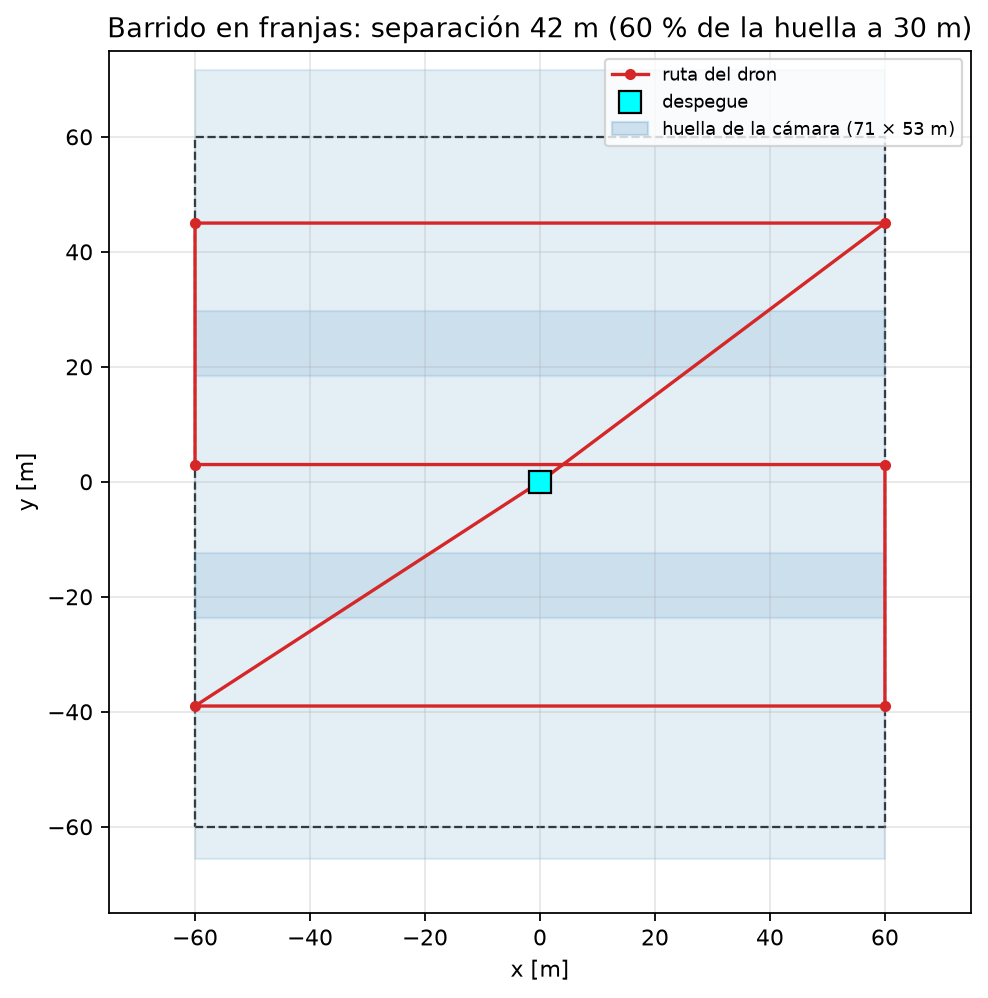
\includegraphics[width=0.65\textwidth]{franjas.png}
\caption{El barrido del proyecto: tres franjas cubren el cuadrado de 120~m con traslape.}
\end{figure}

\section{Volver a mirar: el valor de la información}

Una candidata con confianza intermedia (por ejemplo entre 0.3 y 0.6) es dudosa: puede ser una persona
tapada o una sombra. Bajar a verla desde otro ángulo cuesta tiempo y batería, pero puede convertir una
duda en una persona encontrada (o descartar una falsa alarma). Esa es la estrategia de
\textbf{re-observación}: ¿compensa? Responder esa pregunta con datos es el objetivo de la campaña
experimental (capítulo~\ref{cap:experimental}).

\section{GPS: de metros a latitud y longitud}

La simulación trabaja en metros sobre un plano (ENU); los rescatistas necesitan \textbf{coordenadas GPS}.
La Tierra se modela como un elipsoide (\textbf{WGS84}). La conversión exacta pasa el punto del plano
local a coordenadas cartesianas centradas en la Tierra (ECEF) y de ahí a latitud, longitud y altitud
(\cod{mision/geo.py}).

\begin{figure}[H]
\centering
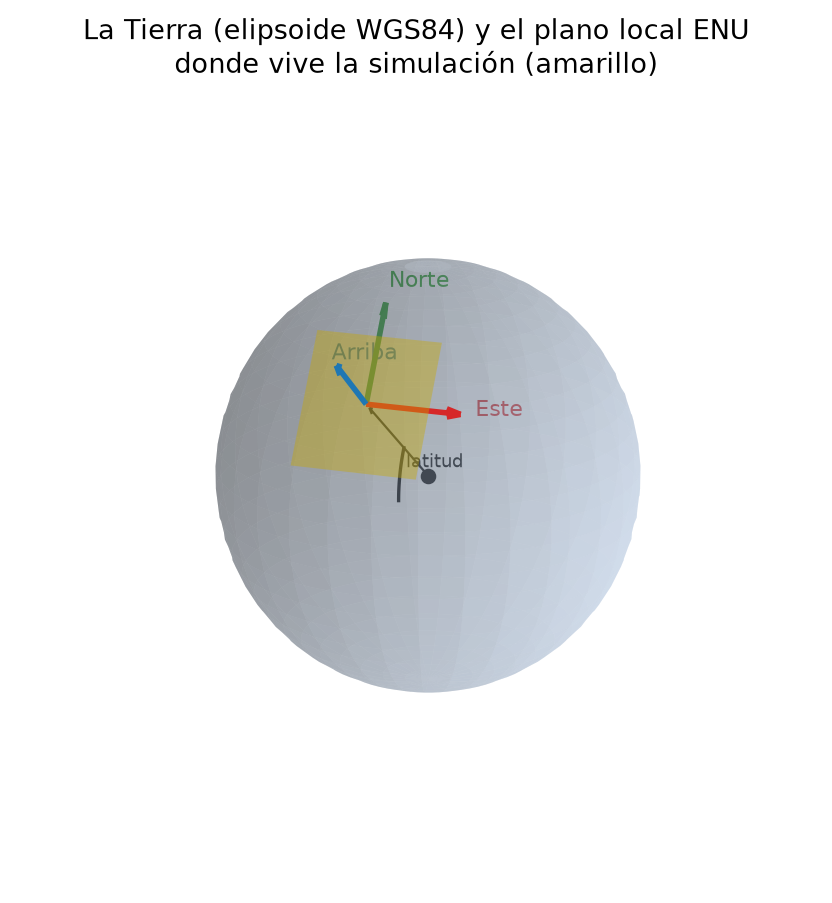
\includegraphics[width=0.55\textwidth]{c_tierra.png}
\caption{El plano local ENU de la simulación es tangente a la Tierra en el origen del mundo.}
\end{figure}

\begin{tecnico}
A 19.5° de latitud, un grado de latitud mide unos 110.8~km y uno de longitud unos 105~km: seis
decimales en las coordenadas equivalen a $\approx$10~cm.
\end{tecnico}

\section{LiDAR}

Un \textbf{LiDAR} mide la distancia al primer obstáculo en muchas direcciones lanzando pulsos láser. Da
una nube de puntos: no sabe \emph{qué} es cada punto, pero sí dónde está. La cámara reconoce personas;
el LiDAR evita chocar.

\begin{figure}[H]
\centering
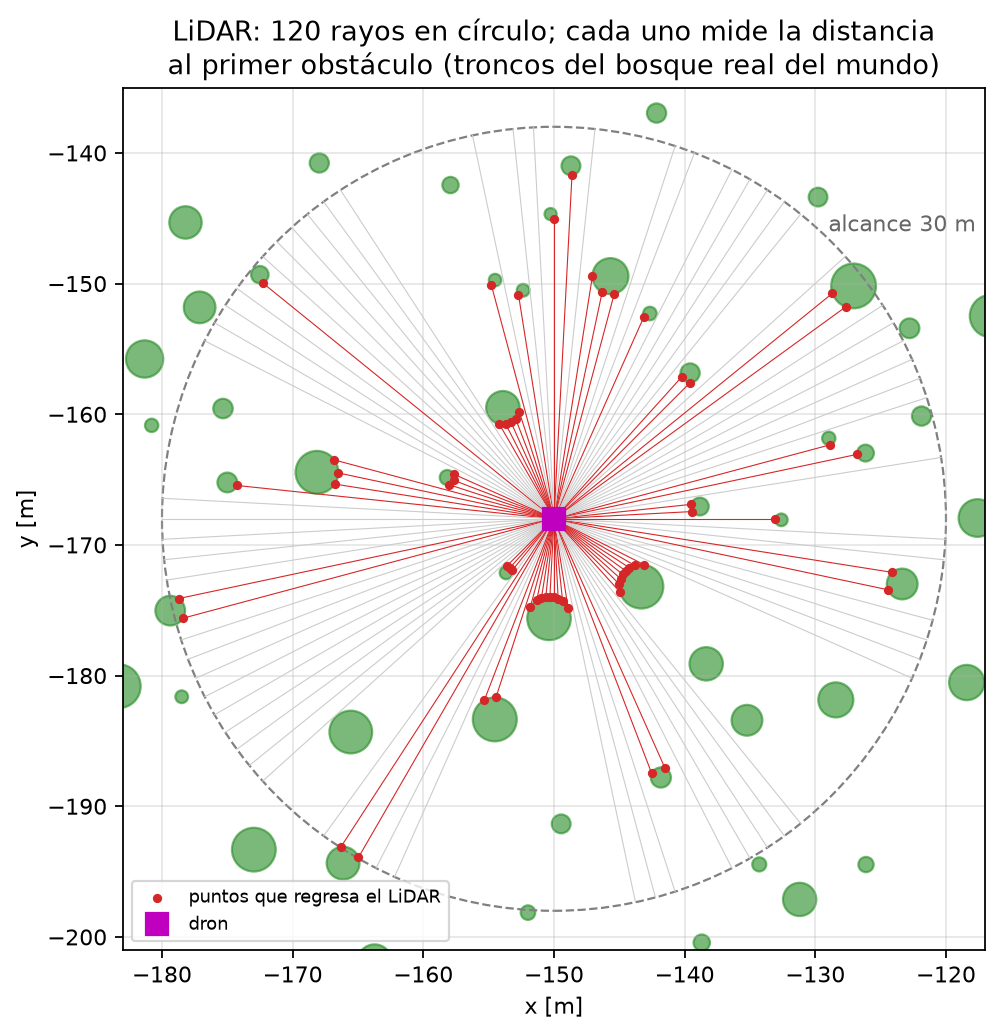
\includegraphics[width=0.55\textwidth]{c_lidar.png}
\caption{Una capa de un LiDAR en un bosque: cada rayo rojo toca un tronco.}
\end{figure}

La evasión del proyecto es reactiva, del tipo VFH: divide las direcciones alrededor del dron en 72
sectores, marca los bloqueados por obstáculos cercanos y toma el sector libre más parecido a la
dirección deseada.

\begin{figure}[H]
\centering
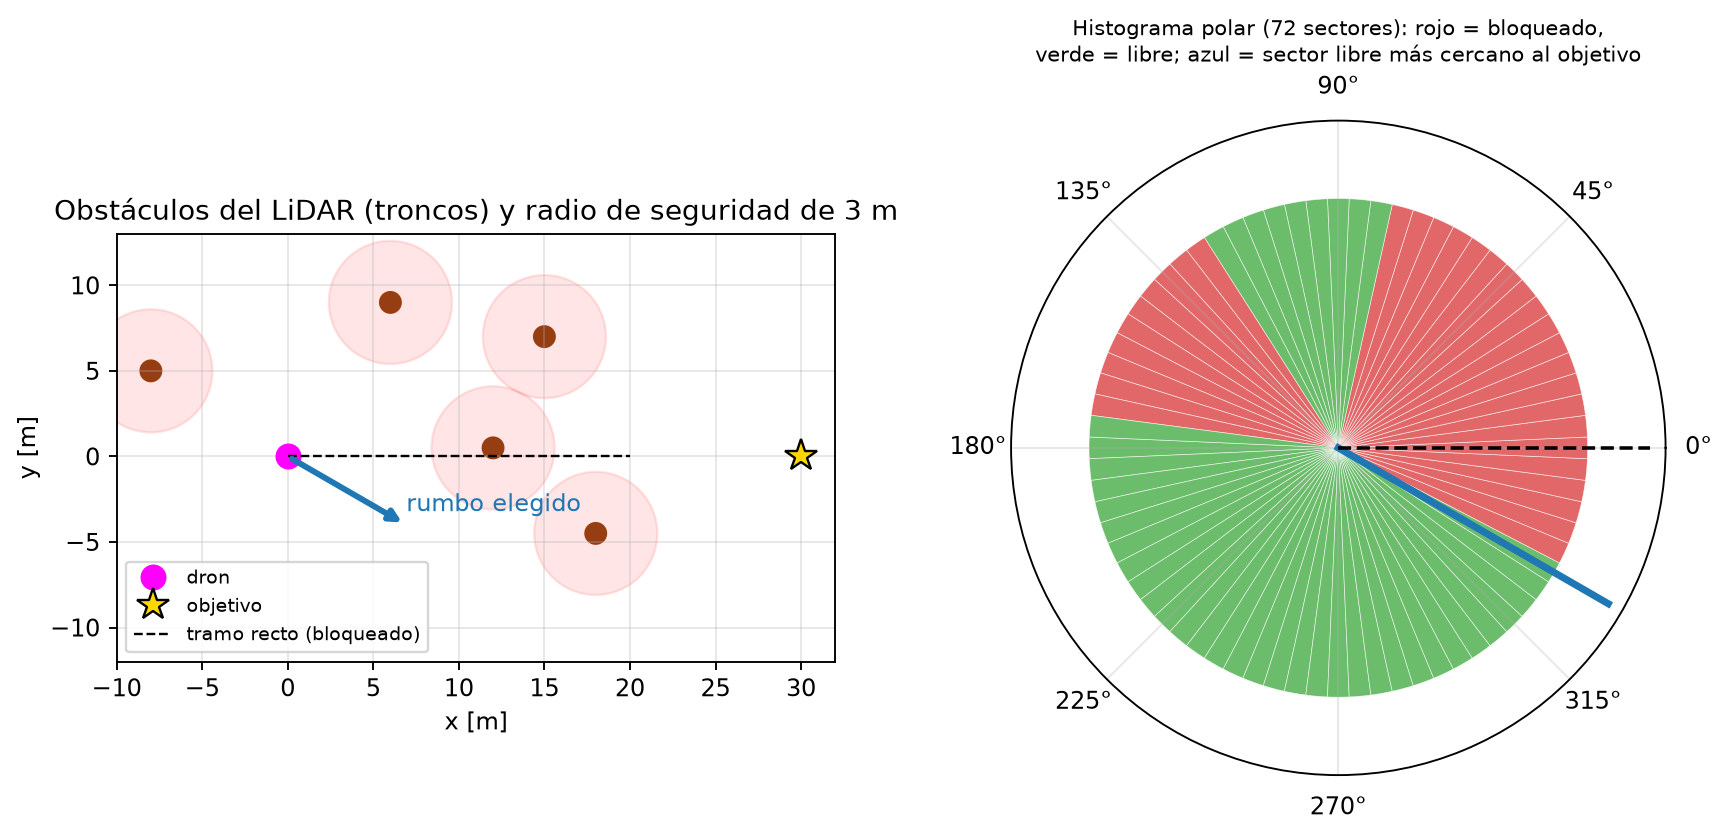
\includegraphics[width=\textwidth]{vfh.png}
\caption{Evasión con histograma polar.}
\end{figure}

\chapter{La misión de búsqueda, pieza por pieza}
\label{cap:mision}

\begin{enpocas}
Cómo está programada la misión (\cod{mision_node}): el barrido, la re-observación de candidatas dudosas
(Algoritmo~1), el cambio a la red neuronal con la consigna adelantada, los avisos GPS, la evasión y las
métricas que se guardan al final.
\end{enpocas}

\section{El ciclo}

La misión corre a 20~Hz. En cada ciclo publica una consigna de posición (\cod{TrajectorySetpoint} en
NED) y el modo \emph{offboard}; tras el primer segundo pide a PX4 cambiar a offboard y armar.

\begin{description}
  \item[Despegue:] sube a la vertical del origen hasta la altura de trabajo (30~m).
  \item[Barrido:] recorre las franjas. La consigna avanza a 3~m/s sin alejarse más de 3~m del
        vehículo (\cod{adelanto_max}).
  \item[Re-observación] (\cod{estrategia:=reobs}): al terminar cada franja, si hay candidatas dudosas
        (confianza entre $s_1 = 0.3$ y $s_2 = 0.6$), va a la más cercana: baja a 20~m, con un
        desplazamiento lateral de 6~m para verla desde otro ángulo, espera 3~s y regresa. Cada candidata
        se re-observa a lo más dos veces (Algoritmo~1).
  \item[Aterrizaje:] al terminar, devuelve el control al piloto (si volaba la red) y aterriza.
  \item[Fin:] calcula las métricas, escribe el JSON y termina; el \emph{launch} se cierra solo.
\end{description}

\section{Con la red neuronal}

Con \cod{controlador:=red}, al llegar a la altura de trabajo la misión cambia al modo \emph{Neural
Control} (el identificador lo da PX4 al registrar el modo) y regresa a offboard antes de aterrizar.
Además manda la \textbf{consigna adelantada} $p_{ref} + 1.6\,v_{ref}$ (1.25 en vertical), que convierte
a la red ---que imita una PD--- en una PD con prealimentación (capítulo~\ref{cap:control-neuronal}). El
registro guarda la consigna sin adelanto.

\begin{leccion}
Se probó suavizar el adelanto con un filtro de 1~s para que en las esquinas la consigna no saltara
4.8~m de lado. Empeoró: el adelanto filtrado seguía apuntando en la dirección vieja y el dron se pasaba
de la esquina (RMSE de la ruta de 0.23 a 0.37~m). Sin filtro es exactamente una PD con prealimentación;
el filtro quedó como opción (\cod{tau_adelanto}) desactivada.
\end{leccion}

\section{Avisos con GPS}

Cuando una candidata se confirma durante el barrido ---confianza acumulada $\ge 0.6$, al menos 10
detecciones fusionadas, dentro del área y a más de 5~m de las ya avisadas--- la misión publica una sola
vez:
\begin{itemize}
  \item \cod{/personas/gps}: \cod{NavSatFix} con latitud, longitud y altitud (\cod{frame_id}
        \cod{persona_k});
  \item \cod{/personas/alerta}: el texto del aviso;
\end{itemize}
ambos con QoS \emph{transient local} (quien se suscriba tarde también los recibe). Además lo escribe en la
terminal y en \cod{~/personas_localizadas.csv}:
\begin{lstlisting}
PERSONA 2 LOCALIZADA 2026-10-23 07:50:56
  GPS: 19.482212, -99.245049  (19°28'55.9"N 99°14'42.2"W)
  Mapa: https://www.google.com/maps?q=19.482212,-99.245049
  Local: (-40.0, 35.2) m   confianza 1.00, 10 detecciones
\end{lstlisting}
y en el JSON del mapa que dibuja MAVProxy.

\begin{figure}[H]
\centering
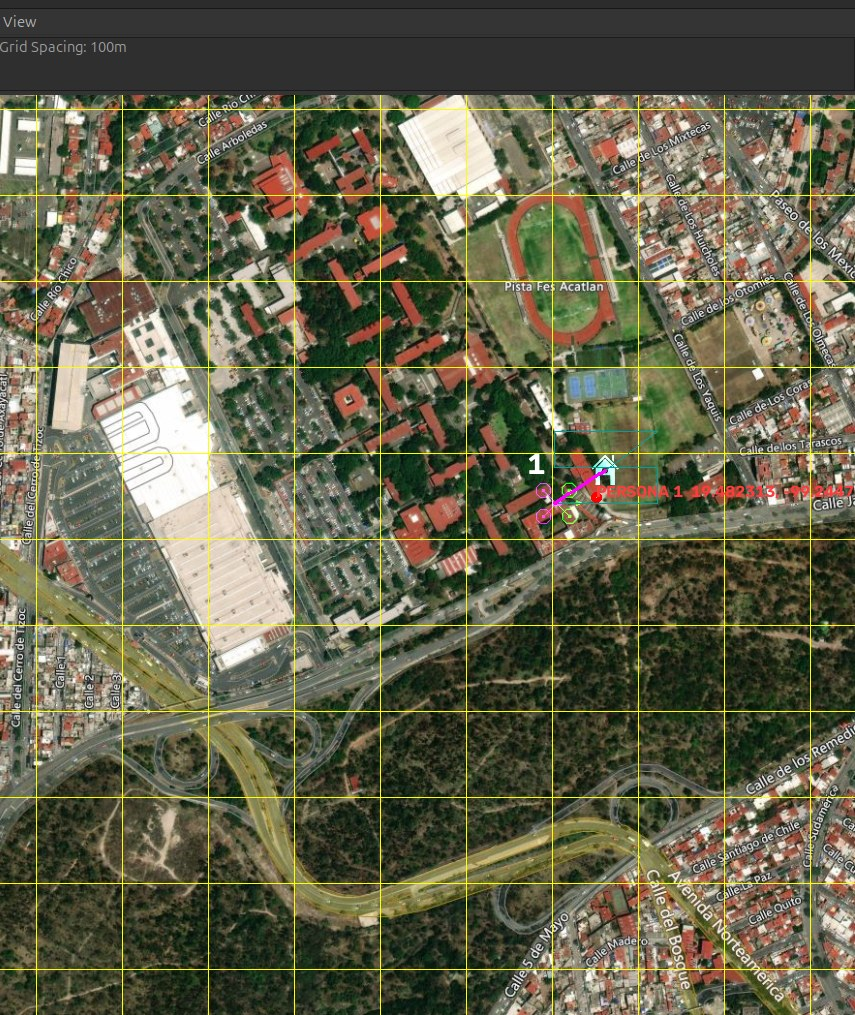
\includegraphics[width=0.55\textwidth]{mapa_personas.jpg}
\caption{El mapa de MAVProxy durante una misión: la persona 1 marcada con sus coordenadas.}
\end{figure}

\begin{leccion}
La primera versión avisó 8 veces para 3 personas: una vista durante el despegue (con 5~m de error),
dos a 250~m (rayos casi horizontales en las vueltas) y otras en grupos de robles. Se agregaron tres
filtros: solo durante el barrido, solo dentro del área y el límite de 60° en el localizador. Quedaron 4 a
6 avisos para 3 personas: las falsas alarmas persistentes de los robles alcanzan las mismas 10
detecciones que las personas reales, así que subir el umbral no las separa. Resolverlas toca al detector
o a la re-observación.
\end{leccion}

\section{Evasión de obstáculos}

Los puntos del LiDAR pasan al marco del mundo con la pose estimada por el piloto (convertida de NED-FRD
a ENU-FLU), se descartan los del suelo y se guardan los cercanos. Si el tramo recto hacia el siguiente
punto pasa a menos de 3~m de un obstáculo a la altura del dron, la consigna toma el rumbo libre más
cercano o sube (\cod{mision/evasion.py}, el mismo algoritmo del capítulo anterior). A 30~m sobre copas de
6.5~m no actúa durante el barrido: protege los tramos bajos y cualquier cambio de altura o de bosque.

\section{Métricas}

Al terminar, la misión compara las candidatas con la verdad (\cod{metricas.py}) y guarda en el JSON:
\begin{longtable}{>{\raggedright\arraybackslash}p{5cm}p{10cm}}
\toprule
\cod{personas_localizadas} & personas con una candidata detectada a menos de 5~m (asignación uno a uno) \\
\cod{falsas_alarmas} & candidatas detectadas que no corresponden a nadie \\
\cod{error_localizacion_m} & distancia media entre persona y candidata \\
\cod{rmse_seguimiento} & distancia RMS del dron a la ruta durante el barrido (sin los desvíos) \\
\cod{reobservaciones}, \cod{duracion_s} & desvíos hechos y duración \\
\cod{por_min_detecciones} & lo mismo exigiendo 1, 3, 5 o 10 detecciones fusionadas \\
\cod{avisos}, \cod{trayectoria}, \cod{eventos} & avisos GPS, trayectoria a 25~Hz y cambios de estado \\
\bottomrule
\end{longtable}

\chapter{Volar con PX4 o con ArduPilot}
\label{cap:pilotos}

\begin{enpocas}
Cómo se conecta la misión a cada piloto automático, cómo corre la red neuronal en cada uno, y la estación
de tierra (MAVProxy) con sus ventanas y su mapa.
\end{enpocas}

\section{Con PX4 (\texorpdfstring{\texttt{piloto:=px4}}{piloto:=px4}, por omisión)}

El \emph{launch} abre Gazebo con el bosque (sin la configuración de PX4), arranca el agente uXRCE-DDS en
el puerto 8888 y PX4 SITL (\cod{px4_sitl_neural}, \emph{airframe} 4099) conectado a ese Gazebo
(\cod{PX4_GZ_STANDALONE}). La misión habla con PX4 por ROS~2: lee \cod{/fmu/out/vehicle_odometry} y
\cod{/fmu/out/vehicle_status_v1}, y publica \cod{/fmu/in/trajectory_setpoint},
\cod{/fmu/in/offboard_control_mode} y comandos (\cod{/fmu/in/vehicle_command}). La red corre dentro de
PX4, en \cod{mc_nn_control}.

\section{Con ArduPilot (\texorpdfstring{\texttt{piloto:=ardupilot}}{piloto:=ardupilot})}

\begin{itemize}
  \item ArduCopter 4.7.2 se lanza directo (sin MAVProxy ni ventana propia) con los parámetros de
        \cod{config/ardupilot/x500.parm}, el \emph{home} en el origen del mundo y el vehículo dentro del
        mundo a 1~kHz.
  \item \cod{mision_ardupilot} (una subclase de la misión) se conecta por TCP 5760 con MAVLink, vuela en
        GUIDED con \cod{SET_POSITION_TARGET_LOCAL_NED} y publica el estimado del EKF de ArduPilot en
        \cod{/fmu/out/vehicle_odometry}, para que el localizador sea exactamente el mismo.
  \item Con \cod{controlador:=red}, la red corre en \cod{controlador_red} (ROS~2 + gz-transport,
        $\sim$330~Hz, 70~µs por paso) con el estado de Gazebo y manda
        $\omega_i = 1000\sqrt{(a_i+1)/2}$~rad/s. La misión publica ``red'' en \cod{/x500/controlador} y
        \cod{SelectorMotores} deja pasar esos comandos; ArduPilot sigue estimando, recibe las mismas
        consignas y recupera los motores para aterrizar, o si la red deja de publicar 50~ms.
\end{itemize}

\section{La estación de tierra: MAVProxy}

Con GUI, el \emph{launch} abre MAVProxy en su propia terminal, con consola, mapa y el módulo
\cod{mision.mavproxy_trayectoria}, conectado a PX4 por UDP 14550 o a ArduPilot por TCP 5762;
\cod{ventanas_sitl} acomoda las ventanas (terminal y consola a la izquierda, Gazebo al centro, mapa a la
derecha). El mapa dibuja la ruta planeada, la trayectoria recorrida y cada persona avisada.

\begin{figure}[H]
\centering
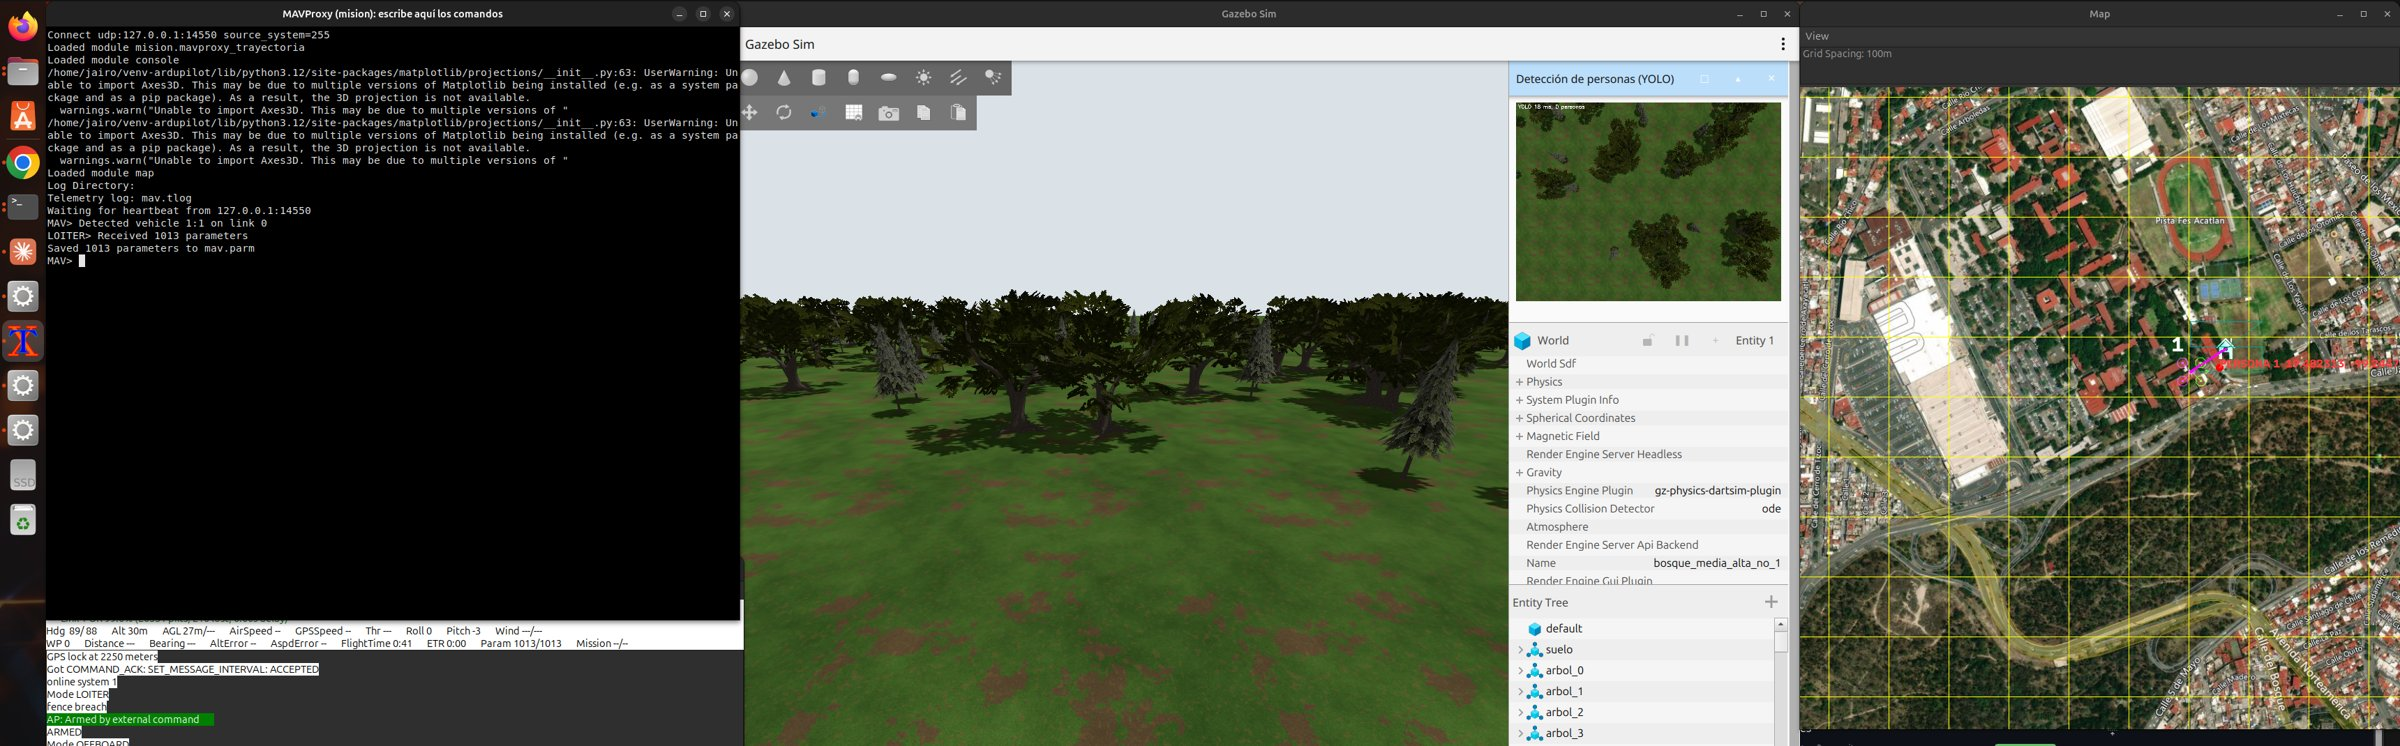
\includegraphics[width=\textwidth]{pantalla_mavproxy.jpg}
\caption{MAVProxy conectado a PX4: la terminal (con el prompt para escribir comandos), la consola, Gazebo
y el mapa.}
\end{figure}

\begin{longtable}{>{\raggedright\arraybackslash}p{5cm}p{10cm}}
\toprule
\textbf{Comando en MAVProxy} & \textbf{Efecto} \\ \midrule \endhead
\cod{mode LOITER} / \cod{mode RTL} / \cod{mode LAND} & detenerse, regresar al despegue, aterrizar \\
\cod{arm throttle} / \cod{disarm} & armar / desarmar \\
\cod{param show MPC_*} & ver parámetros (PX4) \\
\cod{trayectoria borrar|ocultar|mostrar} & dibujo de la trayectoria en el mapa \\
\bottomrule
\end{longtable}

\begin{aviso}
Si tomas el control desde MAVProxy, la misión sigue mandando consignas de offboard (PX4) o GUIDED
(ArduPilot). Al regresar a ese modo el dron retoma la búsqueda.
\end{aviso}

\section{Una simulación a la vez}

El \emph{launch} usa \cod{/clock}, \cod{/camera} y el puerto 8888 del agente. Para correr otra
simulación al mismo tiempo (por ejemplo, otra de ROS en la misma computadora), lánzala en otra partición
de Gazebo y otro dominio de ROS:
\begin{lstlisting}[style=bash]
GZ_PARTITION=busqueda ROS_DOMAIN_ID=7 ros2 launch mision simulacion.launch.py
\end{lstlisting}
Dos PX4 al mismo tiempo no se puede sin cambiar puertos: por eso la campaña corre los vuelos uno por uno.


\part{Experimentos y manos a la obra}
\chapter{La campaña experimental}
\label{cap:experimental}

\begin{enpocas}
Qué preguntas se quieren responder, cómo se diseñan los vuelos para responderlas sin engañarse, la
prueba de Wilcoxon con la corrección de Holm, y lo que dijo la campaña.
\end{enpocas}

\section{Las preguntas}

\begin{description}
  \item[P1.] ¿La re-observación de candidatas dudosas encuentra más personas que el barrido fijo, y
        en qué nivel de oclusión ayuda más?
  \item[P2.] ¿Cuánto cuesta? Tiempo de vuelo, personas por minuto y desvío de la ruta.
  \item[P3.] ¿Qué tan sensible es la misión a un detector más lento o que pierde cuadros
        (\cod{latencia_extra_ms}, \cod{saltar_cuadros})?
  \item[P4.] ¿Cambia algo volar con la red neuronal en vez de la cascada de PX4?
\end{description}

\section{El diseño}

Un \textbf{diseño factorial completo}: todas las combinaciones de oclusión (3), iluminación (2), viento
(2) y estrategia (2), es decir 24 vuelos por semilla con el controlador en cascada. Para P4 se agregan,
en oclusión media y sol alto, los 4 vuelos de la red (con y sin viento, las dos estrategias): 28 vuelos
por semilla.

\begin{lstlisting}[style=bash]
python3 src/mision/scripts/correr_experimentos.py --semillas 30 --salida ~/resultados     # 840 vuelos
python3 src/mision/scripts/correr_experimentos.py --semillas 2 --solo oclusion=media      # una parte
\end{lstlisting}

Cada vuelo es un \cod{ros2 launch} sin interfaz en su propia partición de Gazebo y su dominio de ROS~2,
dura unos 5~minutos y deja un JSON. El programa salta los vuelos que ya tienen JSON, así que se puede
interrumpir y continuar, o ampliar de 5 a 30 semillas.

\begin{consejo}
\textbf{Apareado.} La re-observación y el barrido fijo vuelan \emph{el mismo bosque} (misma semilla,
iluminación y viento). La diferencia entre los dos vuelos de un par se debe a la estrategia y no a que a
uno le tocó un bosque más difícil. Así se necesitan muchos menos vuelos para ver un efecto.
\end{consejo}

\section{Wilcoxon y Holm}

Para cada par se calcula la diferencia $d = \text{reobs} - \text{fija}$ (personas encontradas, por
ejemplo). La \textbf{prueba de rangos con signo de Wilcoxon} pregunta si esas diferencias tienden a ser
positivas, sin suponer que siguen una campana de Gauss: ordena las $|d|$, les pone rango y compara la
suma de los rangos positivos con la de los negativos. Se reporta la mediana de $d$ con un intervalo de
confianza del 95~\% obtenido por remuestreo (\emph{bootstrap}).

Se hacen 12 pruebas (3 oclusiones $\times$ 4 variables). Con tantas, alguna saldría ``significativa'' por
pura suerte; la \textbf{corrección de Holm} lo evita: ordena los valores $p$ de menor a mayor y multiplica
el $k$-ésimo por $(m-k+1)$, sin dejar que bajen.

\begin{lstlisting}[style=bash]
~/venv-mision/bin/python src/mision/scripts/analisis_wilcoxon.py --resultados ~/resultados
~/venv-mision/bin/python src/mision/scripts/analisis_wilcoxon.py --demo        # datos sintéticos
\end{lstlisting}

\begin{aviso}
Una sola semilla no compara estrategias: en el primer bosque la re-observación puede ganar o perder por
casualidad. Las conclusiones salen de los pares, no de un vuelo bonito.
\end{aviso}

\section{Resultados}

\IfFileExists{capitulos/resultados_campana.tex}{%
Las tablas siguientes las genera \cod{herramientas/tabla_campana.py} a partir de los JSON de
\cod{~/resultados}; se regeneran al agregar semillas.

% generado por herramientas/tabla_campana.py con 2 corridas
Corridas analizadas: 2 (semillas 1--1).
\begin{table}[H]\centering\small
\begin{tabular}{lllrrrrrrr}
\toprule
\textbf{Control} & \textbf{Oclusión} & \textbf{Estrategia} & $n$ & \textbf{Encontradas} & \textbf{FA} & \textbf{FA$_{10}$} & \textbf{Avisos} & \textbf{Duración (s)} & \textbf{RMSE (m)} \\ \midrule
cascada & baja & fija & 1 & 1/1 & 14.0 & 2.0 & 2.0 & 237 & 0.069 \\
cascada & baja & reobs & 1 & 1/1 & 22.0 & 6.0 & 5.0 & 278 & 0.279 \\
\bottomrule
\end{tabular}
\caption{Promedios por condición. FA: falsas alarmas con una detección; FA$_{10}$: con al menos 10; avisos GPS por vuelo.}
\label{tab:campana-medias}
\end{table}
\begin{table}[H]\centering\small
\begin{tabular}{llrrcrr}
\toprule
\textbf{Oclusión} & \textbf{Variable} & $n$ & \textbf{Mediana $d$} & \textbf{IC 95~\%} & $p$ & $p_{Holm}$ \\ \midrule
baja & personas & 1 & 0.000 & [0.000, 0.000] & 1.000 & 1.000 \\
baja & personas/min & 1 & -0.037 & [-0.037, -0.037] & 1.000 & 1.000 \\
baja & RMSE (m) & 1 & 0.210 & [0.210, 0.210] & 1.000 & 1.000 \\
baja & falsas alarmas & 1 & 8.000 & [8.000, 8.000] & 1.000 & 1.000 \\
media & personas & 0 & -- & [--, --] & -- & -- \\
media & personas/min & 0 & -- & [--, --] & -- & -- \\
media & RMSE (m) & 0 & -- & [--, --] & -- & -- \\
media & falsas alarmas & 0 & -- & [--, --] & -- & -- \\
alta & personas & 0 & -- & [--, --] & -- & -- \\
alta & personas/min & 0 & -- & [--, --] & -- & -- \\
alta & RMSE (m) & 0 & -- & [--, --] & -- & -- \\
alta & falsas alarmas & 0 & -- & [--, --] & -- & -- \\
\bottomrule
\end{tabular}
\caption{Re-observación menos barrido fijo, apareado por semilla, iluminación y viento (controlador en cascada).}
\label{tab:campana-wilcoxon}
\end{table}

}{%
\textit{Las tablas se generan con \cod{herramientas/tabla_campana.py} cuando termina la campaña.}
}

\begin{leccion}
\textbf{Las falsas alarmas dependen del umbral.} Con una sola detección cualquier sombra que el detector
confunda una vez cuenta como candidata (10 a 20 por vuelo); exigiendo 10 detecciones fusionadas quedan
pocas, y casi todas son grupos de robles que el detector confunde una y otra vez. Por eso la tabla trae
las dos cifras, y por eso el aviso GPS exige 10.
\end{leccion}

\chapter{Tu primer vuelo, paso a paso}
\label{cap:primer-vuelo}

\begin{enpocas}
Lanzar una misión completa, saber qué mirar en cada ventana, leer el resultado y cambiar una cosa a la
vez.
\end{enpocas}

\section{Antes de empezar}

\begin{itemize}
  \item La instalación del capítulo~\ref{cap:instalacion} ya está hecha y compilada (\cod{colcon build}).
  \item No hay otra simulación de PX4 abierta (comparten el puerto 8888).
  \item Si la campaña está corriendo, espera a que termine o usa otra partición y otro dominio
        (capítulo~\ref{cap:pilotos}).
\end{itemize}

\section{Paso 1: lanzar}

\begin{lstlisting}[style=bash]
source ~/ros2_ws/install/setup.bash
ros2 launch mision simulacion.launch.py
\end{lstlisting}
En unos 30~segundos aparecen Gazebo con el bosque, la terminal y la consola de MAVProxy, y el mapa.
El Tarot 650 despega del origen. La terminal de ROS va diciendo lo que pasa (esta salida es de una
corrida del 23 de octubre, con el x500; con el Tarot los mensajes son los mismos):
\begin{lstlisting}
[mision]: misión fija con controlador cascada: 8 puntos de ruta a 30.0 m
[mision]: despegue -> barrido
PERSONA 1 LOCALIZADA 2026-10-23 08:28:21
  GPS: 19.482273, -99.244990  (19°28'56.2"N 99°14'42.0"W)
[mision]: barrido -> aterrizaje
[mision]: 1/1 personas localizadas, 14 falsas alarmas, error 0.43
[mision]: misión terminada en 237 s; RMSE de seguimiento 0.07 m; registro en ...
\end{lstlisting}

\section{Paso 2: mirar}

\begin{description}
  \item[Gazebo:] el dron, el bosque y, a la derecha, el panel ``Detección de personas'' con la
        imagen de la cámara y los recuadros de YOLO.
  \item[Mapa de MAVProxy:] la ruta en franjas, la trayectoria recorrida y cada persona avisada.
  \item[Terminal:] los avisos con GPS y enlace a Google Maps.
\end{description}

\begin{figure}[H]
\centering
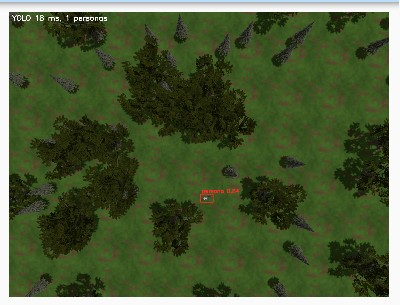
\includegraphics[width=0.85\textwidth]{panel_yolo_personas.jpg}
\caption{El panel de detección durante el barrido.}
\end{figure}

\section{Paso 3: leer el resultado}

\begin{lstlisting}[style=bash]
python3 -c "import json; r=json.load(open('$HOME/resultados/corrida.json')); \
print(r['personas_localizadas'], '/', r['personas'], r['falsas_alarmas'], r['duracion_s'])"
\end{lstlisting}
El significado de cada campo está en la tabla de métricas del capítulo~\ref{cap:mision}.

\section{Paso 4: cambiar una cosa}

\begin{lstlisting}[style=bash]
ros2 launch mision simulacion.launch.py estrategia:=reobs             # con re-observación
ros2 launch mision simulacion.launch.py oclusion:=alta semilla:=4     # bosque denso
ros2 launch mision simulacion.launch.py controlador:=red              # vuela la red neuronal
ros2 launch mision simulacion.launch.py piloto:=ardupilot             # con ArduPilot
ros2 launch mision simulacion.launch.py vehiculo:=x500                # con el x500 de PX4
ros2 launch mision simulacion.launch.py gui:=false salida:=$HOME/r.json   # sin ventanas
\end{lstlisting}

\begin{ejercicio}
Vuela la semilla 1 en oclusión alta con \cod{estrategia:=fija} y luego con \cod{reobs}. ¿Cuántas
personas encontró cada una, y cuánto tardó? Luego repite con la semilla 2. ¿Se mantiene la conclusión?
\end{ejercicio}

\begin{ejercicio}
Vuela con \cod{latencia_extra_ms:=300}. ¿Cuánto crece el error de localización? ¿Por qué? (Pista: a
3~m/s, 300~ms son 0.9~m.)
\end{ejercicio}

\section{Si algo falla}

\begin{longtable}{>{\raggedright\arraybackslash}p{5cm}p{10cm}}
\toprule
\textbf{Síntoma} & \textbf{Causa y remedio} \\ \midrule \endhead
El dron no despega & PX4 no recibe la odometría o el agente no arrancó: revisa que no haya otra
simulación en el puerto 8888 (\cod{pgrep -a MicroXRCE}). \\
La memoria se llena en minutos & Gazebo cargó \cod{GstCameraSystem}; el \emph{launch} lo evita, no
uses \cod{make px4_sitl gz_...} para estas misiones. \\
Ninguna persona encontrada & ¿El detector cargó los pesos? Busca \cod{[detector]} en la terminal y
mira \cod{/detecciones}. \\
Quedan ventanas abiertas & \cod{pkill -f mavproxy}; el \emph{launch} normalmente las cierra. \\
Con \cod{vehiculo:=x500} y \cod{controlador:=red} PX4 vuela mal & PX4 lleva compilada la red del Tarot;
reinstala la del x500 con \cod{instalar_px4.sh} (capítulo~\ref{cap:tarot650}). \\
\bottomrule
\end{longtable}

\chapter{Referencia rápida}

\begin{enpocas}
Los argumentos del \emph{launch}, los parámetros de la misión, los tópicos y los programas, en tablas
para consultar.
\end{enpocas}

\section{Argumentos de \texorpdfstring{\texttt{simulacion.launch.py}}{simulacion.launch.py}}

\begin{longtable}{>{\raggedright\arraybackslash}p{4.2cm}>{\raggedright\arraybackslash}p{3.3cm}p{7.5cm}}
\toprule
\textbf{Argumento} & \textbf{Por omisión} & \textbf{Qué hace} \\ \midrule \endhead
\cod{oclusion} & media & baja, media, alta: cobertura de copas 15, 45, 75~\% \\
\cod{iluminacion} & alta & alta (mediodía) o baja (sombras largas) \\
\cod{viento} & no & si: 4~m/s medios con ráfagas \\
\cod{semilla}, \cod{personas} & 1, (1 a 3) & bosque y número de personas \\
\cod{estrategia} & fija & fija o reobs (Algoritmo~1) \\
\cod{piloto} & px4 & px4 o ardupilot \\
\cod{controlador} & cascada & cascada (del piloto) o red \\
\cod{altura}, \cod{velocidad}, \cod{lado} & 30, 3, 120 & m, m/s, m \\
\cod{pesos}, \cod{umbral} & YOLO26s, 0.25 & modelo del detector y confianza mínima \\
\cod{pesos_red} & (la instalada) & pesos de la red para \cod{controlador_red} (ArduPilot) \\
\cod{latencia_extra_ms}, \cod{saltar_cuadros} & 0, 0 & degradación artificial del detector (P3) \\
\cod{gui}, \cod{mavproxy} & true, true & ventanas de Gazebo y estación de tierra \\
\cod{salida} & \cod{~/resultados/corrida.json} & registro del vuelo \\
\cod{px4}, \cod{ardupilot} & \cod{~/PX4-Autopilot}, \cod{~/ardupilot} & dónde están los pilotos \\
\bottomrule
\end{longtable}

\section{Parámetros de \texorpdfstring{\texttt{mision\_node}}{mision\_node}}

\begin{longtable}{>{\raggedright\arraybackslash}p{4.2cm}>{\raggedright\arraybackslash}p{3.3cm}p{7.5cm}}
\toprule
\textbf{Parámetro} & \textbf{Por omisión} & \textbf{Qué hace} \\ \midrule \endhead
\cod{adelanto_max} & 3.0~m & distancia máxima de la consigna por delante del dron \\
\cod{huella} & 70~m & ancho de la huella para planear franjas \\
\cod{s1}, \cod{s2} & 0.3, 0.6 & confianza de una candidata dudosa \\
\cod{max_reobs}, \cod{altura_reobs}, \cod{espera_reobs} & 2, 20~m, 3~s & re-observación \\
\cod{radio_acierto}, \cod{min_detecciones} & 5~m, 1 & para las métricas \\
\cod{tiempo_max} & 900~s & corta la misión si se pasa \\
\cod{prealimentacion} & $-1$ (auto) & consigna adelantada con la red \\
\cod{tau_adelanto} & 0~s & filtro del adelanto (desactivado) \\
\cod{n_aviso} & 10 & detecciones para avisar con GPS \\
\cod{registro_personas} & \cod{~/personas_localizadas.csv} & bitácora de avisos \\
\cod{origen_gps} & 19.4826, $-99.2447$, 2250 & origen del mundo \\
\cod{evasion}, \cod{radio_evasion}, \cod{alcance_evasion} & true, 3~m, 20~m & evasión con LiDAR \\
\bottomrule
\end{longtable}

\section{Tópicos}

\begin{longtable}{>{\raggedright\arraybackslash}p{5.5cm}>{\raggedright\arraybackslash}p{3.6cm}p{5.9cm}}
\toprule
\textbf{Tópico} & \textbf{Tipo} & \textbf{Quién lo publica} \\ \midrule \endhead
\cod{/camera}, \cod{/camera_info} & Image, CameraInfo & Gazebo (puente) \\
\cod{/detecciones} & Detection2DArray & detector \\
\cod{/camera_yolo} & Image & detector (imagen con recuadros) \\
\cod{/detector/latencia_ms} & Float32 & detector \\
\cod{/personas/estimaciones} & Detection3DArray & localizador (cada detección) \\
\cod{/personas/candidatas} & Detection3DArray & localizador (fusionadas) \\
\cod{/personas/gps}, \cod{/personas/alerta} & NavSatFix, String & misión \\
\cod{/x500/consigna} & PointStamped & misión \\
\cod{/x500/lidar/points} & PointCloud2 & Gazebo (puente) \\
\cod{/fmu/out/vehicle_odometry} & VehicleOdometry & PX4 (o \cod{mision_ardupilot}) \\
\cod{/fmu/in/trajectory_setpoint} & TrajectorySetpoint & misión \\
\bottomrule
\end{longtable}

\section{Programas}

\begin{longtable}{>{\raggedright\arraybackslash}p{5.5cm}p{9.5cm}}
\toprule
\textbf{Programa} & \textbf{Para qué} \\ \midrule \endhead
\cod{scripts/generar_mundo.py} & bosque por factores \\
\cod{scripts/generar_vehiculo.py} & modelos x500\_busqueda (PX4 y ArduPilot) \\
\cod{scripts/importar_personas.py} & modelos de personas desde Gazebo Fuel \\
\cod{scripts/capturar_dataset.py}, \cod{preparar_datos.py}, \cod{entrenar_detector.py} & datos y entrenamiento del detector \\
\cod{scripts/correr_experimentos.py}, \cod{analisis_wilcoxon.py} & campaña y estadística \\
\cod{scripts/instalar_px4.sh} & copia la red y el \emph{airframe} a PX4 \\
\cod{codigo/nn_imitacion.py}, \cod{ppo_refinamiento.py}, \cod{exportar_tflite.py} & entrenamiento y exportación de la red \\
\cod{mision/prueba_neural.py} & escalones con la red en SITL \\
\bottomrule
\end{longtable}

\chapter{Lo que se verificó y lo que falta}

\begin{enpocas}
Los problemas que aparecieron al llevar el diseño a la computadora, cómo se resolvieron, y lo que queda
pendiente.
\end{enpocas}

\section{Diferencias con el diseño original}

El diseño original del que parte el proyecto tenía nueve detalles que no funcionaban tal cual. Todos
están corregidos en el paquete:
\begin{enumerate}
  \item La etiqueta \cod{v1.17.0} de PX4 no existe; se usa la rama \cod{release/1.17}.
  \item El sensor de la cámara se llama \cod{imager}, no \cod{camera}.
  \item \cod{VehicleStatus} es versionado: el tópico es \cod{/fmu/out/vehicle_status_v1}.
  \item En \cod{x500_mono_cam_down} la cámara está 10~cm \emph{arriba} del centro y ve el propio
        vehículo; aquí va 25~cm abajo.
  \item La configuración de Gazebo de PX4 carga \cod{GstCameraSystem}, que acumula cuadros si el
        codificador se atora: 110~MB/s y el sistema se queda sin memoria en minutos. Aquí Gazebo
        arranca sin él.
  \item \cod{MC_NN_THRST_COEF} trabaja con revoluciones por segundo, no rpm, y faltaban
        \cod{MC_NN_MIN_RPM} y \cod{THR_MDL_FAC}; los valores correctos están en el \emph{airframe}
        4099 y los verifican las pruebas.
  \item La masa del x500 completo es 2.114~kg, no 2.0.
  \item \cod{exportar_tflite.py} usaba \cod{--salida} como nombre del símbolo en C; el módulo exige
        \cod{control_net_tflite}.
  \item PX4 marca sus mensajes con el reloj de pared, no con el de Gazebo; el localizador estima el
        desfase con el mínimo de (llegada $-$ marca).
\end{enumerate}

\section{Lo que se comprobó}

\begin{itemize}
  \item Los programas de modelo, localización, imitación, PPO y exportación reproducen las tablas y
        salidas de referencia (el TFLite difiere de numpy en $1.1\times10^{-6}$).
  \item El detector ajustado: AP50 0.954 en validación; el YOLO de COCO no encontraba a nadie.
  \item La red mejorada: sesgo estacionario de 25.9 a 2.1~cm y misión en 211~s en vez de 427~s.
  \item Las coordenadas GPS de los avisos coinciden con el GPS de PX4, el \emph{home} de ArduPilot y el
        mapa de MAVProxy (prueba \cod{test_origen_gps_igual_al_del_mundo}).
  \item \cod{colcon test}: las 8 pruebas del paquete pasan.
\end{itemize}

\section{Pendientes}

\begin{itemize}
  \item \textbf{Falsas alarmas persistentes.} Grupos de robles que el detector confunde en muchos
        cuadros. Reentrenar con esos ``negativos difíciles'' es el siguiente paso.
  \item \textbf{PPO.} Ya no diverge, pero no mejora a la imitación; falta una recompensa que premie lo
        que la imitación no sabe hacer (por ejemplo, rechazar viento).
  \item \textbf{Seguimiento de cámara en la GUI.} \cod{/gui/follow} no funciona con esta interfaz.
  \item \textbf{Campaña completa.} Con 5 semillas se ven tendencias; las 30 semillas del diseño dan la
        potencia estadística para P1.
\end{itemize}


\appendix
\chapter{Glosario}

\begin{description}[style=nextline,leftmargin=0.6cm]
  \item[AP50, AP50-95] Precisión promedio de un detector, contando como acierto un recuadro que se
        traslapa al menos 50~\% (o promediando de 50 a 95~\%) con el verdadero.
  \item[ArduPilot / ArduCopter] Piloto automático de código abierto; ArduCopter es su versión para
        multirrotores.
  \item[Armar] Habilitar los motores para que puedan girar.
  \item[Barrido] Recorrer una zona en franjas paralelas para verla toda.
  \item[Bootstrap] Remuestrear los datos muchas veces para estimar la incertidumbre de una cifra.
  \item[Candidata] Posible persona en el mapa: varias detecciones fusionadas en un punto.
  \item[Cascada] Lazos de control anidados: posición afuera, velocidad, actitud y velocidad angular
        adentro.
  \item[Consigna] Lo que se pide al controlador (posición, velocidad).
  \item[Consigna adelantada] Consigna desplazada en la dirección del movimiento para que un PD siga
        una referencia móvil sin atraso.
  \item[Cobertura de copas] Fracción del suelo tapada por árboles vistos desde arriba.
  \item[Detector] Red que encuentra objetos en una imagen y los marca con recuadros.
  \item[Diseño factorial] Experimento que prueba todas las combinaciones de los factores.
  \item[EKF] Filtro de Kalman extendido: estima posición y orientación combinando sensores.
  \item[ENU / NED] Este-Norte-Arriba (ROS, Gazebo) y Norte-Este-Abajo (PX4, aviación).
  \item[Falsa alarma] Candidata que no corresponde a ninguna persona.
  \item[FLU / FRD] Marcos del cuerpo: Frente-Izquierda-Arriba (ROS) y Frente-Derecha-Abajo (PX4).
  \item[Gazebo] Simulador de robots con física, render y sensores.
  \item[GUIDED] Modo de ArduPilot en el que obedece consignas de una computadora.
  \item[Holm] Corrección que ajusta los valores $p$ cuando se hacen muchas pruebas a la vez.
  \item[Huella] Rectángulo del suelo que ve la cámara.
  \item[Imitación] Entrenar una red para que copie las salidas de otro controlador.
  \item[LiDAR] Sensor que mide distancias con pulsos láser en muchas direcciones.
  \item[MAVLink] Protocolo de mensajes entre pilotos automáticos y estaciones de tierra.
  \item[MAVProxy] Estación de tierra en terminal, con consola y mapa.
  \item[Máquina de estados] Programa organizado en etapas con reglas para pasar de una a otra.
  \item[Neural Control] Modo de PX4 en el que una red neuronal manda los motores directamente.
  \item[Offboard] Modo de PX4 en el que obedece consignas de una computadora.
  \item[Oclusión] Que algo tape lo que se quiere ver.
  \item[PPO] Algoritmo de aprendizaje por refuerzo que mejora una política con pasos pequeños.
  \item[Prealimentación] Sumar al control lo que ya se sabe que se necesita (por ejemplo, la velocidad
        de la referencia), sin esperar a que haya error.
  \item[PX4] Piloto automático de código abierto.
  \item[Re-observación] Volver a mirar una candidata dudosa desde más cerca y otro ángulo.
  \item[RMSE] Raíz del error cuadrático medio.
  \item[ROS~2] Conjunto de herramientas para que los programas de un robot se comuniquen por tópicos.
  \item[Semilla] Número que fija los resultados al azar; con la misma semilla sale lo mismo.
  \item[SITL] \emph{Software in the loop}: el piloto automático real corriendo contra un simulador.
  \item[TFLite] Formato compacto de redes neuronales para microcontroladores.
  \item[Tópico] Canal con nombre por el que los nodos de ROS~2 se mandan mensajes.
  \item[uXRCE-DDS] Puente entre PX4 y ROS~2.
  \item[VFH] Histograma polar de campo vectorial: evasión que busca la dirección libre más cercana.
  \item[Wilcoxon] Prueba estadística para diferencias apareadas que no supone una campana de Gauss.
  \item[WGS84] Elipsoide que modela la forma de la Tierra para el GPS.
  \item[YOLO] Familia de detectores de objetos que mira la imagen una sola vez.
\end{description}


\end{document}
